\documentclass{tnreport}
%\documentclass[stage1a]{tnreport} % If you are in 1nd year
%\documentclass[stage2a]{tnreport} % If you are in 2nd year
%\documentclass[confidential]{tnreport} % If you are writing confidential report
%\documentclass[english]{tnreport} % If you are writing your report in english
%\documentclass[contratpro]{tnreport} % If you are in contrat pro

\def\reportTitle{Industrialisation de la chaîne de valeur d'une ESN} % Titre du mémoire
\def\reportLongTitle{Industrialisation de la chaîne de valeur d'une ESN : développement du capital humain et innovation technologique} % Titre plus long du mémoire

\def\reportAuthor{David Guichard}
\def\reportAuthorEmail{\email{david.guichard@telecomnancy.eu}} % Courriel de l'élève

% This is an example, for a report with several students as authors
%\def\reportAuthor{Jon Snow\\ Samwell Tarly}
%\def\reportAuthorEmail{\email{jon@castleblack.com}\\ \email{tarly@casteblack.com}} % Courriel de l'élève

\def\reportAuthorAddress{5, rue Pierre d'Artagnan} % Adresse de l'élève
\def\reportAuthorCity{92350 Le Plessis-Robinson} % Adresse (cont.) de l'élève
\def\reportAuthorPhone{06 20 32 37 21} % Téléphone de l'élève

%\def\reportIndustrialSupervisor{Prénom Nom} % Prénom Nom de l'encadrant industriel
\def\reportSupervisor{Maxime Bauer} % Prénom Nom de l'encadrant industriel (en entreprise ou laboratoire)
\def\reportAcademicSupervisor{Thibault Cholez} % Prénom Nom de l'encadrant académique

% For PIDR ?
%\def\reportSupervisor{Eddard Stark} % Prénom Nom de l'encadrant industriel
%\def\reportProjectCustomer{Projet réalisé pour l'équipe Night's Watch du laboratoire HBO}

\def\reportCompany{Oxyl} % Nom de l'entreprise d'accueil
\def\reportCompanyAddress{19-21, rue du 8 Mai 1945}  % Adresse de l'entreprise
\def\reportCompanyCity{94110 Arcueil} % Adresse (cont.) de l'entreprise
\def\reportCompanyPhone{09 72 60 09 87} % Téléphone de l'entreprise
\def\reportCompanyLogoPath{figures/Oxylgroupe} % Logo officiel Oxyl
%\def\reportSecondCompanyLogoPath{figures/logo.png} % Deuxième logo d'entreprise si besoin

\def\place{Nancy} % Ville pour la signature pour l'engagement anti-plagiat
\def\date{\today} % Date pour la signature de l'engagement anti-plagiat

\usepackage{tikz}
\usetikzlibrary{shapes.geometric,arrows.meta,positioning,calc,fit}
\usepackage{multirow}

% Harmonisation typographique de la commande \code (noms de fichiers, fonctions, variables)
\DeclareUrlCommand\code{\def\UrlFont{\footnotesize\ttfamily}}

% --- Définitions du Glossaire et des Acronymes ---
\newglossaryentry{ESN}{
    name={ESN},
    description={Entreprise de Services du Numérique. Société de conseil et d'ingénierie délivrant des prestations logicielles en régie ou au forfait}
}
\newglossaryentry{SDLC}{
    name={SDLC},
    description={\textit{Software Development Life Cycle}. Cycle de vie global du développement logiciel, de l'analyse du besoin au maintien en condition opérationnelle}
}
\newglossaryentry{LLM}{
    name={LLM},
    description={\textit{Large Language Model}. Grand modèle de traitement automatique du langage fondé sur des réseaux de neurones profonds (\textit{Transformers})}
}
\newglossaryentry{CLI}{
    name={CLI},
    description={\textit{Command-Line Interface}. Interface utilisateur textuelle manipulée et exécutée en ligne de commande}
}
\newglossaryentry{OCP}{
    name={OCP},
    description={\textit{Oracle Certified Professional}. Certification professionnelle de référence sanctionnant la maîtrise avancée de la plateforme Java SE}
}
\newglossaryentry{OCA}{
    name={OCA},
    description={\textit{Oracle Certified Associate}. Certification industrielle validant l'acquisition des fondamentaux de la programmation Java}
}
\newglossaryentry{SOLID}{
    name={SOLID},
    description={Ensemble de cinq principes de conception orientée objet (\textit{Single responsibility, Open-closed, Liskov substitution, Interface segregation, Dependency inversion}) favorisant la maintenabilité et l'extensibilité du code}
}
\newglossaryentry{TJM}{
    name={TJM},
    description={Taux Journalier Moyen. Métrique tarifaire de référence représentant le coût de facturation journalier d'un ingénieur consultant}
}
\newglossaryentry{ROI}{
    name={ROI},
    description={\textit{Return on Investment} (Retour sur Investissement). Indicateur financier mesurant la rentabilité et les gains économiques générés par un investissement}
}
\newglossaryentry{RAG}{
    name={RAG},
    description={\textit{Retrieval-Augmented Generation}. Technique combinant un mécanisme de recherche documentaire et un modèle génératif pour contextualiser précisément les réponses}
}
\newglossaryentry{MR}{
    name={MR / PR},
    description={\textit{Merge Request} / \textit{Pull Request}. Demande formelle de fusion d'une branche de fonctionnalités vers la branche principale, soumise à une revue de code collaborative}
}
\newglossaryentry{REST}{
    name={REST},
    description={\textit{Representational State Transfer}. Style architectural standardisé fondé sur les protocoles et verbes HTTP pour la communication entre services web}
}
\newglossaryentry{DTO_DAO}{
    name={DTO / DAO},
    description={\textit{Data Transfer Object} / \textit{Data Access Object}. Patrons de conception dédiés respectivement au transport de données structurées et à l'abstraction de la couche de persistance}
}
\newglossaryentry{Vendor_Lockin}{
    name={Vendor Lock-in},
    description={Enfermement ou dépendance propriétaire. Situation de dépendance technologique où un système ne peut changer de fournisseur sans surcoûts majeurs}
}

\begin{document}

\maketitle
\pagenumbering{roman}

\insertAntiPlagiarismAgreement{Guichard, David}{322119809}{figures/anonymous_company-logo}{0.2}
                            % {Nom, Prénom}{n°étu}{image signature}{scale signature} 
% You may insert several agreement in case of multiple authors
%\insertAntiPlagiarismAgreement{Tarly, Samwell}{2014031142}{figures/anonymous_company-logo}{0.2}

\cleardoublepage

\makesecondtitle

\section*{Remerciements}
\addcontentsline{toc}{chapter}{Remerciements}

Je tiens à exprimer ma profonde gratitude à l'ensemble des personnes qui ont contribué, par leur encadrement, leurs conseils avisés et leur soutien, au bon déroulement et à la réussite de ce Projet de Fin d'Études au sein du Groupe Oxyl.

Mes remerciements s'adressent tout particulièrement à :

\begin{itemize}
    \item \textbf{Maxime \textsc{Bauer}}, mon tuteur de stage et reviewer senior, pour sa disponibilité constante, sa bienveillance et l'exigence constructive de ses revues de code lors des sprints du backend de la plateforme de quiz. Ses précieux retours d'ingénierie et sa vision logicielle ont grandement enrichi ma pratique du développement ;
    \item \textbf{Selena \textsc{Hind Woodward}}, Directrice des Ressources Humaines d'Oxyl, pour sa confiance accordée dès le processus de recrutement, son accueil chaleureux et pour ses enseignements particulièrement formateurs sur les méthodes agiles et la dynamique collaborative au sein de l'entreprise ;
    \item \textbf{Clément \textsc{Dubois}}, pour son coaching technique rigoureux lors des sprints backend et ses revues de code pointues, qui ont constitué un moteur constant d'apprentissage et d'élévation des standards de qualité ;
    \item \textbf{Jeremy \textsc{Roca}}, développeur senior et chef d'équipe sur le projet de l'usine logicielle agentique, pour la qualité de son accueil, son \textit{onboarding} méthodique et sa pédagogie dans la transmission des enjeux d'architecture du moteur ;
    \item \textbf{Jordan \textsc{Peter}} et \textbf{Alexandre \textsc{Danty}}, développeurs seniors et relais d'équipe au sein du projet de l'usine logicielle, pour leur disponibilité, leur écoute et leurs conseils techniques pertinents lors des phases de conception et de synchronisation d'équipe ;
    \item \textbf{Mathéo \textsc{Allard}}, Scrum Master des projets internes, pour son pilotage précieux et ses orientations claires sur les attendus du projet d'usine logicielle, ainsi que pour ses conseils avisés sur les bonnes pratiques de revue de code et le déroulement des \textit{dailys} ;
    \item \textbf{Pierre \textsc{Valat}}, collègue stagiaire et compagnon de route sur l'ensemble de ce parcours -- de la plateforme de quiz jusqu'à l'usine logicielle -- pour cette collaboration quotidienne stimulante, l'entraide technique et la dynamique d'équipe partagée ;
    \item \textbf{Thibault \textsc{Cholez}}, mon enseignant-référent et tuteur académique à TELECOM Nancy, pour son suivi attentif, sa disponibilité et ses conseils méthodologiques tout au long de ce projet de fin d'études.
\end{itemize}

Enfin, j'adresse mes sincères remerciements à l'ensemble des collaborateurs du Groupe Oxyl pour leur accueil et la richesse des échanges au quotidien, au corps professoral et à l'équipe pédagogique de TELECOM Nancy pour la solidité de la formation délivrée, ainsi qu'à ma famille et mes proches pour leur soutien indéfectible tout au long de mon cursus d'ingénieur.


\cleardoublepage

\section*{Avant-propos}
\addcontentsline{toc}{chapter}{Avant-propos}

Ce Projet de Fin d'Études chez Oxyl s'inscrit au carrefour de mon parcours d'ingénieur et d'une vision professionnelle mûrement réfléchie.

Dès le choix de ma spécialisation à TELECOM Nancy, j'ai délibérément privilégié la filière \textit{Logiciel Embarqué}. Ce choix stratégique répondait à une volonté de construire un socle de compétences bas-niveau et architectural solide, indispensable pour appréhender les systèmes complexes avec une réelle rigueur d'ingénierie.

Cette passerelle entre socle logiciel et intelligence artificielle s'est dessinée dès mon stage de deuxième année au laboratoire CRAN, à travers la conception d'une architecture cognitive en \textit{Deep Learning} pour un bras robotique en cobotique industrielle. Elle s'est ensuite consolidée lors de mon semestre d'échange académique à Madrid, dédié à l'approfondissement théorique et pratique du \textit{Machine Learning}. Mon intégration chez Oxyl est venue parachever cette démarche, en mettant à profit cette double culture pour concevoir une usine logicielle optimisée par l'automatisation agentique.

Ce mémoire marque ainsi une étape charnière : à l'avenir, j'envisage de poursuivre dans l'automatisation des processus d'entreprise par les systèmes agentiques. Une ambition guidée par la conviction que l'efficacité de l'IA appliquée dépend avant tout de la robustesse du socle en développement logiciel sur lequel elle s'appuie.

\vspace{1cm}
\begin{flushright}
    \textit{David \textsc{Guichard}}\\
    \textit{Le Plessis-Robinson, le 18 août 2026}
\end{flushright}


\cleardoublepage

\renewcommand{\baselinestretch}{0.5}\normalsize
\tableofcontents
\renewcommand{\baselinestretch}{1.0}\normalsize
\cleardoublepage

\pagenumbering{arabic}
\setcounter{page}{1}

\chapter{Introduction Générale}
\label{chap:introduction}

\section*{Contexte sectoriel : La métamorphose du modèle des ESN}

Le secteur des Entreprises de Services du Numérique (ESN) traverse une phase de mutation structurelle sans précédent, impulsée par l'émergence et la maturation rapide de l'intelligence artificielle générative et des architectures agentiques. Historiquement, le modèle économique de l'ingénierie logicielle de prestation reposait en grande partie sur l'assistance technique en régie, valorisée au temps passé. Aujourd'hui, la dynamique du marché impose une transition accélérée vers des modèles au forfait et des engagements au résultat. Dans ce paradigme, les cycles de livraison sont drastiquement raccourcis, la prévisibilité des charges devient un enjeu critique de rentabilité, et la moindre dérive dans l'estimation des délais fait peser un risque direct sur la pérennité de la relation client.

Parallèlement, l'automatisation progressive des phases élémentaires du cycle de développement logiciel (\textit{Software Development Life Cycle} -- SDLC) bouleverse la gestion des talents. Les tâches jadis confiées aux développeurs juniors sont de plus en plus prises en charge par des agents d'assistance au code, fermant l'accès aux missions traditionnelles d'intégration pour les profils en début de carrière. En outre, le marché fait face à une dichotomie marquée au sein de la clientèle : tandis qu'une fraction exige une vélocité accrue portée par l'IA, une part significative d'entreprises -- notamment dans les secteurs réglementés ou stratégiques -- interdit formellement l'utilisation d'outils d'IA tiers pour prévenir tout risque de fuite de données sensibles ou d'atteinte à la propriété intellectuelle. Pour une ESN, l'équation impose ainsi de maintenir une rigueur méthodologique humaine irréprochable tout en intégrant l'automatisation logicielle de pointe.

\section*{L'écosystème Oxyl et sa stratégie d'innovation}

Dans cet environnement concurrentiel tendu, \reportCompany{} a fait le choix stratégique de se positionner très tôt comme une entreprise pionnière sur l'intégration de l'intelligence artificielle dans ses processus d'ingénierie logicielle. L'ambition d'Oxyl repose sur une vision duale : acquérir une expertise de premier plan sur les systèmes agentiques pour concevoir des produits à haute valeur ajoutée, tout en décuplant la performance opérationnelle de ses propres consultants en mission.

Cette posture d'innovation s'accompagne d'une politique de formation et de gestion du capital humain ciblée. Afin de maintenir une dynamique perpétuelle de veille technologique et de renouvellement intellectuel, Oxyl privilégie le recrutement par la continuité de stage de fin d'études. L'accueil d'élèves-ingénieurs permet d'éprouver en temps réel les dernières avancées académiques et techniques face aux exigences concrètes de la production industrielle.

\section*{Le double défi d'ingénierie : Standardisation du capital humain et du capital technique}

Pour concrétiser cette vision industrielle, le projet d'ingénierie mené durant ce stage s'articule autour de deux axes fondamentaux et complémentaires :

\begin{enumerate}
    \item \textbf{La standardisation et la valorisation du capital humain (Le volet compétences) :} Face aux exigences accrues des clients, l'excellence technique des collaborateurs doit être démontrable et certifiée. L'obtention de certifications reconnues par l'industrie -- à l'instar des titres Oracle (\textit{Oracle Certified Associate} -- OCA, \textit{Oracle Certified Professional} -- OCP) pour l'écosystème Java/JEE, ou de l'accréditation \textit{AWS Certified Cloud Practitioner} -- constitue un puissant gage de crédibilité. Pour soutenir cet impératif, une plateforme web sur-mesure a été conçue en Spring Core et Angular. Pensée à la fois comme un \textit{moyen} (un projet grandeur nature formant aux standards d'architecture) et comme un \textit{but} (un outil d'entraînement, de passage d'examens blancs et de suivi statistique pour les encadrants), cette plateforme structure la montée en compétences et la gouvernance pédagogique interne.
    \item \textbf{La standardisation et l'indépendance du capital technique (Le volet Usine Logicielle) :} Pour automatiser les tâches répétitives du cycle de vie logiciel sans subir les aléas des solutions propriétaires, Oxyl a initié le développement d'une \og Usine Logicielle \fg{} agentique en TypeScript, régie par des spécifications formelles en Markdown (prompts, descriptions d'incidents et règles d'architecture logicielle propre). Face à la volatilité des coûts de facturation des jetons (\textit{tokens}), aux impératifs de confidentialité et à la diversité des infrastructures clientes, un enjeu architectural majeur est apparu : garantir l'agnosticité complète du moteur. Il s'agissait de découpler l'infrastructure d'exécution vis-à-vis des fournisseurs de modèles de langage (OpenAI, Anthropic Claude, Google, modèles locaux) et des gestionnaires de dépôts et de tickets (GitHub, GitLab, Gitea, Jira, Bitbucket).
\end{enumerate}

\section*{Problématique et objectifs du Projet de Fin d'Études}

L'intersection entre l'exigence d'un socle d'ingénierie rigoureux et l'impératif d'industrialisation automatisée soulève la problématique centrale de ce mémoire :

\begin{center}
    \setlength{\fboxsep}{10pt}
    \fbox{\parbox{0.9\textwidth}{\centering\bfseries\itshape
    Dans un marché des ESN contraint par le passage au forfait et la transformation des métiers du développement par l'IA, comment concilier la standardisation du capital humain (gage de qualité et de maîtrise des fondamentaux) et l'industrialisation d'une usine logicielle agentique agnostique pour pérenniser la rentabilité et l'indépendance technologique de l'entreprise ?
    }}
\end{center}

\section*{Cadre méthodologique et dynamique d'équipe}

La réalisation de ces travaux s'est inscrite dans deux contextes méthodologiques complémentaires, illustrant la diversité des modes d'organisation en ingénierie logicielle :

\begin{itemize}
    \item \textbf{Le projet de la plateforme d'évaluation (Équipe de 4 stagiaires) :} Mené \textit{from scratch}, le projet a débuté selon des cycles Scrum hebdomadaires rythmés par des revues de code individuelles exigeantes, conditionnant la validation de chaque incrément. La phase finale sur le développement front-end s'est ensuite déroulée en semi-autonomie sous forme de flux Kanban (points quotidiens, découpage atomique des tâches). Cette configuration a constitué un exercice pratique immersif sur la gestion de la dette technique, l'arbitrage entre vélocité et maintenabilité, et le respect d'échéances strictes.
    \item \textbf{Le projet Usine Logicielle (Organisation Agile d'entreprise) :} Intégré au sein d'une équipe structurée par un \textit{Scrum Master} avec un backlog rigoureusement priorisé, le travail a suivi des rituels réguliers (\textit{dailies}, synchronisations hebdomadaires). La culture de qualité logicielle y a été renforcée par une pratique intensive de la revue de code collective (une à deux sessions quotidiennes), permettant d'aligner en continu les décisions d'architecture et les principes de \textit{Clean Code}.
\end{itemize}

\section*{Synthèse des contributions personnelles}

Bien que s'inscrivant dans une démarche collaborative, mes contributions d'ingénieur ont plus particulièrement porté sur :
\begin{itemize}
    \item Le développement \textit{full-stack} de la plateforme d'évaluation des compétences, notamment la modélisation des entités, les API de gestion des référentiels pédagogiques et l'implémentation des parcours de tests.
    \item La conception et l'implémentation de la couche d'abstraction logicielle au sein de l'Usine Logicielle, spécifiquement l'interopérabilité des connecteurs de gestionnaires de code source (\textit{CodebaseProviders} : GitHub, GitLab, Gitea, Bitbucket) et des systèmes de suivi de tickets (\textit{BacklogProviders} : Jira, GitLab/GitHub Issues).
    \item L'évaluation et la consolidation des patrons de conception (\textit{Design Patterns}) assurant l'extensibilité et la résilience du moteur face à l'hétérogénéité des écosystèmes clients.
\end{itemize}

\section*{Organisation du mémoire}

Le présent mémoire est structuré en cinq chapitres qui retracent la démarche d'ingénierie adoptée :

\begin{itemize}
    \item Le \textbf{Chapitre~\ref{chap:cadre}} détaille le cadre de l'étude, en analysant l'écosystème d'Oxyl, le cycle de vie du consultant, les risques de dépendance technologique (\textit{vendor lock-in}) et la justification stratégique du couplage entre formation et automatisation.
    \item Le \textbf{Chapitre~\ref{chap:quiz}} présente le premier volet consacré à la standardisation du capital humain, en détaillant l'architecture de la plateforme d'évaluation (Spring Core / Angular) et son rôle dans la maîtrise des fondamentaux d'ingénierie.
    \item Le \textbf{Chapitre~\ref{chap:usine_ia}} aborde le second volet dédié au capital technique, à travers l'état de l'art sur l'industrialisation du SDLC par les agents autonomes, la théorie de l'abstraction logicielle et la gestion des contraintes opérationnelles (coûts et sécurité).
    \item Le \textbf{Chapitre~\ref{chap:infra_agnostique}} décrit la mise en œuvre de l'infrastructure agnostique, détaillant les patrons de conception retenus, l'uniformisation des interfaces de programmation et les résultats expérimentaux obtenus.
    \item Le \textbf{Chapitre~\ref{chap:analyse_critique}} propose une analyse critique et systémique du projet, mesurant les retours sur investissement, la réduction des dépendances propriétaires et les perspectives éthiques de l'IA appliquée au génie logiciel.
    \item Enfin, la \textbf{Conclusion Générale} synthétisera les apports du projet et ouvrira sur l'évolution prospective du métier d'ingénieur logiciel.
\end{itemize}

\cleardoublepage

\chapter{Vers une industrialisation de la chaîne de valeur (Le cadre)}
\label{chap:cadre}

\section{L'ESN comme \og usine \fg{} de talent et de code : Présentation d'Oxyl et du cycle de vie du consultant}
\label{sec:usine_talent}

Dans une économie numérique fortement concurrentielle et marquée par l'accélération technologique, le modèle traditionnel des Entreprises de Services du Numérique (ESN) est confronté à un impératif de transformation. Pour répondre aux exigences de rentabilité, de vélocité et d'excellence technique imposées par les donneurs d'ordre, \reportCompany{} a développé un modèle singulier assimilant l'entreprise à une véritable double \og usine \fg{} : d'une part une \og usine de talents \fg{}, chargée de recruter, former et standardiser les compétences d'ingénieurs à haut potentiel, et d'autre part une \og usine de code \fg{}, outillée pour industrialiser la production logicielle grâce aux architectures modernes et à l'automatisation agentique.

\subsection{Présentation du Groupe Oxyl et positionnement stratégique}
\label{subsec:presentation_oxyl}

Fondée initialement en 1995 par Fabrice \textsc{Reby} et des élèves-ingénieurs de l'École Centrale de Lille sous le nom d'\textit{AlphaCSP}, l'entreprise s'est d'abord distinguée par son rôle de pionnière dans l'adoption industrielle des technologies Java/J2EE en France, en nouant des partenariats technologiques de premier plan avec des acteurs historiques tels qu'IBM, BEA Systems ou Borland. Précurseur également dans la diffusion des démarches agiles (notamment Scrum et eXtreme Programming) dès le début des années 2000, la société a fait évoluer sa structure et son identité pour devenir le \textbf{Groupe Oxyl} (Digital Makers).

Aujourd'hui implanté à Arcueil en région parisienne, le groupe rassemble environ $200$~collaborateurs et a réalisé en 2024 un chiffre d'affaires consolidé de près de $20$~millions d'euros. Oxyl se positionne comme un cabinet de conseil en technologies et une ESN de niche à forte valeur ajoutée, axée sur la maîtrise approfondie du cycle de vie logiciel (\textit{Software Development Life Cycle} -- SDLC) : de la conception architecturale au déploiement continu en environnement Cloud, en passant par le développement et le maintien en condition opérationnelle (MCO).

Sur le plan technique, Oxyl concentre son cœur de métier autour de deux écosystèmes majeurs et de leurs extensions industrielles :
\begin{itemize}
    \item \textbf{L'écosystème Java / JEE \& Spring :} architectures distribuées, microservices, optimisation des performances transactionnelles, mapping objet-relationnel et sécurité applicative ;
    \item \textbf{L'écosystème JavaScript / TypeScript :} développement d'applications web réactives modernes (Angular, React, Vue.js, Node.js) ;
    \item \textbf{L'ingénierie Cloud \& DevOps :} conteneurisation (Docker, Kubernetes), infrastructures as Code (Terraform, Ansible), pipelines CI/CD et services managés chez les principaux fournisseurs de Cloud public (Amazon Web Services, Microsoft Azure, Google Cloud Platform) ;
    \item \textbf{L'intelligence artificielle et l'automatisation logicielle :} conception d'architectures agentiques, intégration de modèles de langage (LLM) dans les flux de développement et R\&D sur la résolution autonome de tickets.
\end{itemize}

Face aux grandes entreprises généralistes du secteur (telles que Capgemini, Sopra Steria ou Atos) et aux ESN de taille intermédiaire (comme Zenika ou Ippon Technologies), Oxyl fonde son avantage concurrentiel sur une différenciation stratégique majeure :
\begin{enumerate}
    \item \textbf{L'embauche et l'accélération de jeunes diplômés :} recruter des profils à fort potentiel directement en sortie d'école et leur prodiguer un parcours de formation initial intensif et certifiant, dont l'excellence technique est largement reconnue et plébiscitée par les clients grands comptes ;
    \item \textbf{Une culture incarnée par des actes démontrables :} loin de se limiter à des déclarations de principe marketing, les valeurs d'excellence, de partage et de passion se traduisent par des dispositifs concrets (accompagnement tuteur, code reviews systématiques, colocations d'intégration, TechNights) ;
    \item \textbf{Une avance technologique pionnière sur l'IA :} n'ayant pas attendu l'engouement médiatique généralisé pour s'emparer de l'intelligence artificielle agentique, Oxyl a déjà surmonté en interne sur ses projets de R\&D les défis méthodologiques et architecturaux que la plupart des entreprises découvrent aujourd'hui. Cette maturité permet à Oxyl de se positionner en éclaireur et de partager son expérience éprouvée lors d'interventions, de conférences et de publications techniques ;
    \item \textbf{Une hyper-spécialisation et une proximité humaine :} un ancrage fort en région parisienne et une expertise ciblée sur les architectures d'entreprise (Java/Spring, TypeScript/Angular, Cloud et IA).
\end{enumerate}

Cette expertise s'exprime auprès d'un portefeuille de clients diversifiés, comprenant des grands comptes du secteur bancassurance et de la finance (Allianz Trade, BPCE - Casden, Société Générale, MyMoneyBank), des leaders de l'industrie et des services (Rexel, Lafarge, Eutelsat, JCDecaux, Vinci), ainsi que des éditeurs de logiciels et des startups technologiques (Finance Active, Wedia, PrimaSolutions, Hologarde, Wanaka).

\subsection{Organisation structurelle et modèle d'entreprise libérée}
\label{subsec:organisation_entreprise_liberee}

Pour préserver l'agilité organisationnelle et stimuler l'engagement de ses collaborateurs, Oxyl s'est structurée autour des principes de l'\og entreprise libérée \fg{}. Ce paradigme managérial repose sur l'autonomie, la subsidiarité, la réduction des échelons hiérarchiques intermédiaires et la responsabilisation directe des ingénieurs dans les décisions techniques et la vie de l'entreprise.

La culture d'Oxyl s'articule autour de trois valeurs cardinales :
\begin{itemize}
    \item \textbf{La Passion :} inspirée par la maxime de Confucius (\og \textit{Choisissez un travail que vous aimez et vous n'aurez pas à travailler un seul jour de votre vie} \fg{}), l'entreprise s'attache à recruter des profils sincèrement passionnés par l'ingénierie logicielle et l'innovation ;
    \item \textbf{L'Excellence :} sur un marché exigeant, la qualité de prestation repose sur la rigueur technique, le respect des standards de conception (\textit{Clean Code}, patrons de conception) et une veille technologique continue ;
    \item \textbf{Le Partage :} l'entraide mutuelle entre pairs, la transmission du savoir intergénérationnel et le partage de la valeur créée constituent le socle de la cohésion collective.
\end{itemize}

Sur le plan juridique et opérationnel, le groupe s'appuie sur une structure bicéphale synergique :
\begin{itemize}
    \item \textbf{Sylex (L'entité transverse de support) :} structure regroupant les fonctions centrales de l'entreprise (direction générale, administration des ventes, ressources humaines, gestion financière et comptable, prospection commerciale et logistique événementielle) ;
    \item \textbf{Les entités Oxyl par promotion (Oxyl, Oxyl 16 à 23, Oxyl+) :} regroupement des consultants par promotion d'intégration, garantissant le maintien de cellules à échelle humaine afin de pérenniser les liens de confraternité et le sentiment d'appartenance.
\end{itemize}

La gouvernance opérationnelle s'organise autour d'une équipe de direction resserrée : M. Fabrice \textsc{Reby} (fondateur, apportant sa vision stratégique et son portefeuille commercial), Mme Selena \textsc{Hind-Woodward} (responsable du pôle administratif, RH, relations écoles et suivi des carrières), M. Georges \textsc{Coudray} (responsable du pôle commercial et du staffing des consultants), ainsi que M. Maxime \textsc{Bauer} (directeur technique, assurant l'encadrement technologique, la supervision des formations et le pilotage des projets internes de R\&D).

\subsection{L'« usine de talents » : De la sélection à l'excellence certifiée}
\label{subsec:usine_talents}

Le concept d'\og usine de talents \fg{} résume la démarche hautement industrialisée et reproductible mise en place par Oxyl pour transformer des étudiants ingénieurs en consultants immédiatement opérationnels et armés face aux exigences les plus pointues de l'industrie.

\subsubsection{Un processus de sélection ciblé et rigoureux}
Le recrutement constitue le premier maillon de cette chaîne de valeur. Présente activement dans les grandes écoles d'ingénieurs à travers plus de $40$~conférences techniques annuelles, Oxyl attire chaque année plus de $2\,000$~candidatures. Le processus de sélection suit un entonnoir strict à plusieurs étapes :
\begin{enumerate}
    \item \textbf{Test technique initial en ligne (1 heure) :} évaluation des compétences fondamentales en algorithmique et en programmation (taux de sélection : environ $2$ candidats retenus sur $5$) ;
    \item \textbf{Entretien de qualification culturelle :} échange téléphonique mené par un collaborateur pour évaluer la passion du candidat, sa curiosité et son adéquation aux valeurs humaines de l'entreprise (taux d'élimination : environ $30\,\%$) ;
    \item \textbf{Test pratique de développement (1 heure) \& Débriefing technique :} réalisation d'un développement concret sur la base d'un mini cahier des charges, suivi d'une soutenance technique avec un référent pour analyser la démarche d'ingénierie et le raisonnement adopté ;
    \item \textbf{Entretien de synthèse managérial :} validation finale de l'embauche en stage de fin d'études avec les managers du groupe.
\end{enumerate}
Au terme de ce filtre, environ $40$~stagiaires sont intégrés chaque année, répartis en promotions régulières selon leur date d'arrivée. J'ai pour ma part intégré la promotion d'\textbf{avril 2026}. Afin de faciliter l'accueil et l'installation en région parisienne des élèves-ingénieurs issus d'écoles régionales (à l'instar de TELECOM Nancy), Oxyl propose un parc d'appartements en colocation situés à proximité du siège, accélérant ainsi la cohésion d'équipe dès les premiers jours.

\subsubsection{Le parcours de formation initiale standardisé}
Durant les trois premiers mois du stage, l'ensemble des recrues suit un programme de formation intensive conçu pour homogénéiser le niveau technique et bâtir des réflexes d'ingénierie irréprochables. Ce parcours s'articule autour de deux composantes majeures :

\paragraph{1. La validation par les certifications officielles :}
Loin d'un simple apprentissage déclaratif, Oxyl impose la validation de certifications industrielles reconnues internationalement, faisant office de tiers de confiance indiscutable pour les clients (voir Annexe~\ref{annexe:certifications}) :
\begin{itemize}
    \item \textit{Oracle Certified Associate (OCA) Java SE 8 Programmer I :} maîtrise rigoureuse des mécanismes fondamentaux du langage (cycle de vie, typage, modélisation objet, gestion des exceptions) -- attestation officielle présentée en Figure~\ref{fig:certificat_oca} (Annexe~\ref{annexe:certifications}) ;
    \item \textit{Oracle Certified Professional (OCP) Java SE 21 Developer :} assimilation poussée des paradigmes avancés (programmation fonctionnelle, Streams, concurrence, I/O non bloquantes, modules JPMS) ;
    \item \textit{AWS Certified Cloud Practitioner :} acquisition des bases de l'architecture Cloud, des modèles de sécurité partagée et des services managés d'Amazon Web Services -- accréditation officielle présentée en Figure~\ref{fig:certificat_aws} (Annexe~\ref{annexe:certifications}).
\end{itemize}
Cette préparation s'appuie sur la plateforme interne \textbf{MyNewroFactory (MNF)} (entraînement quotidien de $1$~heure le matin et examens blancs surveillés chaque vendredi après-midi).

\paragraph{2. Le projet fil rouge « NewroFactory » (L'apprentissage par l'épreuve) :}
En parallèle de l'étude théorique, chaque stagiaire doit redévelopper en autonomie une version complète de l'application de formation. Découpé en $8$~sprints itératifs, le projet force l'ingénieur à concevoir l'application d'abord en code bas niveau natif (CLI en Java pur, Servlets, JDBC), pour lui faire ressentir concrètement les limitations architecturales avant d'introduire successivement les couches d'abstraction industrielles (pools HikariCP, inversion de contrôle avec Spring Core, MVC, programmation orientée aspect -- AOP, ORM Hibernate/JPA, Spring Security, puis exposition en API RESTful et interface front-end). Chaque sprint est validé lors d'une revue de code (\textit{code review}) collective et intransigeante menée par la direction technique, où le respect des principes de \textit{Clean Code} (SOLID, DRY, KISS, YAGNI) est systématiquement audité.

\begin{figure}[htbp]
\centering
\begin{tikzpicture}[
    scale=0.88,
    transform shape,
    font=\sffamily\scriptsize,
    phasebox/.style={draw=blue!80!black, fill=blue!6, rounded corners=3pt, align=center, inner sep=6pt, line width=0.7pt, minimum width=3.3cm, minimum height=1.3cm},
    detailbox/.style={draw=gray!50, fill=gray!5, rounded corners=2pt, align=left, inner sep=4pt, font=\sffamily\tiny, text width=3.1cm},
    certbox/.style={draw=teal!80!black, fill=teal!8, rounded corners=2pt, align=center, inner sep=4pt, font=\sffamily\bfseries\tiny},
    patharrow/.style={-{Latex[length=3mm]}, thick, draw=blue!80!black},
    forkarrow/.style={-{Latex[length=2.5mm]}, thick, draw=teal!80!black}
]

    % Phase 1 : Recrutement
    \node[phasebox] (p1) at (0, 0) {\textbf{\normalsize 1. Sélection}\\[1pt]\textit{Filtre d'Excellence}};
    \node[detailbox, below=0.25cm of p1] (d1) {
        $\bullet$ $>2000$ candidatures / an\\
        $\bullet$ Test algo en ligne (1h)\\
        $\bullet$ Entretien culturel RH\\
        $\bullet$ Test dev pratique \& soutenance\\
        $\bullet$ \textbf{$\sim$40 admis} en promo PFE
    };

    % Phase 2 : Formation & PFE
    \node[phasebox, fill=teal!6, draw=teal!80!black] (p2) at (4.0, 0) {\textbf{\normalsize 2. PFE \& Formation}\\[1pt]\textit{3 mois d'accélération}};
    \node[detailbox, below=0.25cm of p2] (d2) {
        $\bullet$ \textbf{Projet NewroFactory} :\\
        \phantom{..} 8 sprints \textit{from scratch}\\
        \phantom{..} (CLI $\rightarrow$ Spring $\rightarrow$ Angular)\\
        $\bullet$ Revues de code quotidiennes\\
        $\bullet$ Entraînement MNF ($1\text{h}$/jour)
    };
    \node[certbox, below=0.15cm of d2] (cert) {\textbf{Certifications Validées :}\\Oracle OCA/OCP Java $\cdot$ AWS Cloud};

    % Phase 3 : Double trajectoire
    \node[phasebox, fill=orange!8, draw=orange!80!black, minimum width=3.4cm] (p3a) at (8.4, 0.85) {\textbf{\small Parcours « Padawan »}\\[1pt]\textit{Régie Client supervisée}};
    \node[detailbox, right=0.15cm of p3a, text width=2.4cm] (d3a) {
        $\bullet$ Binômage avec un \textit{Jedi}\\
        $\bullet$ Écosystèmes grands comptes\\
        $\bullet$ Pré-embauche CDI
    };

    \node[phasebox, fill=purple!8, draw=purple!80!black, minimum width=3.4cm] (p3b) at (8.4, -1.0) {\textbf{\small Pôle R\&D / Usine IA}\\[1pt]\textit{Projets Internes Innovants}};
    \node[detailbox, right=0.15cm of p3b, text width=2.4cm] (d3b) {
        $\bullet$ Usine logicielle agentique\\
        $\bullet$ Banc d'essai industriel\\
        $\bullet$ Outillage \& vitrine R\&D
    };

    % Phase 4 : Apprentissage continu
    \node[draw=blue!80!black, fill=blue!10, rounded corners=3pt, align=center, inner sep=4pt, font=\sffamily\bfseries\tiny, fit={(d3a) (d3b) (p3a) (p3b)}] (box3) {};
    % re-draw nodes to be on top
    \node[phasebox, fill=orange!8, draw=orange!80!black, minimum width=3.4cm] at (8.4, 0.85) {\textbf{\small Parcours « Padawan »}\\[1pt]\textit{Régie Client supervisée}};
    \node[phasebox, fill=purple!8, draw=purple!80!black, minimum width=3.4cm] at (8.4, -1.0) {\textbf{\small Pôle R\&D / Usine IA}\\[1pt]\textit{Projets Internes Innovants}};

    % Connecteurs
    \draw[patharrow] (p1) -- (p2);
    \draw[forkarrow] (p2.east) -- ++(0.4,0) |- (p3a.west);
    \draw[forkarrow] (p2.east) -- ++(0.4,0) |- (p3b.west);

    % Cadre global formation continue
    \node[draw=gray!60, dashed, rounded corners=4pt, fit={(p1) (d1) (p2) (cert) (p3a) (d3a) (p3b) (d3b)}, inner sep=8pt, label={[font=\sffamily\bfseries\scriptsize, text=blue!80!black]below:Intelligence Collective \& Formation Continue : MNF permanent $\cdot$ TechNights mensuelles $\cdot$ Café Tech $\cdot$ Veille collaborative}] {};

\end{tikzpicture}
\caption{Pipeline d'industrialisation du capital humain : du recrutement d'élite aux trajectoires opérationnelles chez Oxyl}
\label{fig:pipeline_talents_oxyl}
\end{figure}

\subsection{Le cycle de vie du collaborateur et la dynamique d'apprentissage continu}
\label{subsec:cycle_de_vie_formation_continue}

Comme l'illustre la Figure~\ref{fig:pipeline_talents_oxyl}, à l'issue de cette phase d'accélération initiale de trois mois, le modèle d'Oxyl oriente les consultants vers deux trajectoires opérationnelles complémentaires selon les besoins stratégiques :
\begin{itemize}
    \item \textbf{Le parcours « Padawan » en immersion client :} l'ingénieur est introduit en régie chez un client de l'ESN, sous le tutorat bienveillant d'un consultant senior d'Oxyl (le \og Jedi \fg{}). Ce dispositif, proposé sans refacturation additionnelle durant le stage, garantit une intégration sereine dans des écosystèmes industriels complexes et sécurise l'embauche en CDI à l'issue du cursus.
    \item \textbf{Le parcours R\&D et Projets Internes :} l'ingénieur rejoint l'équipe interne de développement d'Oxyl, dédiée à la conception de solutions innovantes et d'outils d'assistance logicielle (tels que l'extension \textit{OxaPocket} ou l'\textit{Usine Logicielle} agentique). Ce pôle constitue un véritable banc d'essai pour tester les ruptures technologiques et sert de vitrine de savoir-faire pour l'entreprise.
\end{itemize}

Ce cycle de vie professionnel est entretenu tout au long de la carrière du collaborateur par des dispositifs pérennes d'intelligence collective :
\begin{itemize}
    \item \textbf{L'entraînement continu sur MyNewroFactory (MNF) :} la plateforme reste accessible et utilisée tout au long de la carrière des consultants pour la montée en compétences continue, l'entretien des connaissances pointues et la préparation aux qualifications techniques lors du staffing chez de nouveaux clients ;
    \item \textbf{Les TechNights mensuelles :} conférences internes organisées le jeudi soir au siège, où les consultants en mission présentent des retours d'expérience (REX) ou explorent de nouveaux paradigmes (ex. Rust, Kotlin, Claude Code, architectures agentiques) ;
    \item \textbf{Les Café Tech :} ateliers réguliers de veille technique en binômes ;
    \item \textbf{Le portail de veille collective :} base de connaissances collaborative permettant de solliciter les experts internes et de capitaliser sur les solutions éprouvées en mission.
\end{itemize}

En instaurant cette rigueur méthodologique dès l'intégration, Oxyl standardise son capital humain. Cette première étape est la condition indispensable pour aborder le second volet de sa chaîne de valeur : l'industrialisation du capital technique et la mise en place d'une \og usine de code \fg{} automatisée par l'intelligence artificielle.

\section{Problématique double : Analyse de la dépendance technologique (vendor lock-in) et de la fragilité du socle de compétences}
\label{sec:problematique_double}

L'ambition d'Oxyl d'articuler son modèle autour d'une double \og usine \fg{} (de talents et de code) s'inscrit au cœur d'une tension structurelle du secteur informatique. D'un côté, le capital humain fait face à une érosion de la maîtrise des couches basses de l'ingénierie logicielle ; de l'autre, le capital technique est exposé à un risque critique d'enfermement propriétaire face à l'avènement des modèles d'intelligence artificielle générative. La pérennité et la compétitivité de l'entreprise reposent ainsi sur la résolution conjointe de cette double problématique.

\subsection{La fragilité du socle de compétences : du développeur de surface à l'auditeur critique}
\label{subsec:fragilite_competences}

Un paradoxe frappant caractérise la formation contemporaine des jeunes diplômés en informatique : alors qu'ils sont initiés très tôt à des frameworks modernes de haut niveau, une proportion significative d'élèves-ingénieurs intègre le monde professionnel avec une compréhension purement superficielle et strictement utilitaire des concepts. Trop souvent, l'apprentissage privilégie l'usage magique des abstractions (annotations, bibliothèques prêtes à l'emploi) au détriment d'une compréhension intime de ce qui s'exécute \og sous le capot \fg{} (gestion de la mémoire JVM, cycle de vie des objets, mécanismes transactionnels, concurrence non-bloquante ou requêtage SQL natif).

Cette dérive cognitive est aujourd'hui amplifiée par l'omniprésence des assistants de programmation génératifs (tels que GitHub Copilot ou ChatGPT). En générant instantanément des blocs de code fonctionnels en apparence, ces outils installent une illusion de compétence qui masque les lacunes structurelles. L'ingénieur devient alors un simple assembleur de composants qu'il ne maîtrise pas, s'exposant à des risques majeurs :
\begin{itemize}
    \item \textbf{L'introduction de failles invisibles et insidieuses :} des anomalies architecturales, des vulnérabilités de sécurité ou des fuites de ressources qui échappent aux tests unitaires de surface et ne se manifestent qu'en production sous forte charge ou lors d'attaques ciblées ;
    \item \textbf{L'incapacité à maintenir et faire évoluer des systèmes patrimoniaux (\textit{legacy}) :} chez les clients grands comptes, les consultants d'Oxyl sont fréquemment confrontés à des architectures hétérogènes, parfois anciennes ou atypiques. L'adaptation rapide à ces contextes exige une solide culture des concepts fondamentaux pour comprendre rapidement les contraintes sous-jacentes et intervenir avec pertinence ;
    \item \textbf{L'incapacité à auditer le code produit par des tiers ou des agents :} un développeur ne possédant qu'une compréhension moyenne ne peut identifier les erreurs subtiles d'implémentation.
\end{itemize}

Face à ce constat, l'obligation d'un apprentissage \textit{from scratch} (de la programmation système et JDBC brut jusqu'aux architectures d'entreprise) s'impose comme une nécessité absolue pour forger des ingénieurs capables d'appréhender les moindres détails techniques et d'exercer un regard critique intransigeant.

\subsection{Le risque d'enfermement technologique (\textit{vendor lock-in}) : l'impératif d'une usine logicielle agnostique}
\label{subsec:risque_vendor_lock_in}

Parallèlement à la qualification du capital humain, l'automatisation de la chaîne de production logicielle par l'intelligence artificielle soulève un défi d'indépendance technologique sans précédent. Si le verrouillage technologique (\textit{vendor lock-in}) a toujours existé dans l'histoire de l'informatique, il s'accentue de manière critique avec les solutions d'IA générative et voit ses impacts potentiels fortement aggravés par les tensions géopolitiques contemporaines et les impératifs de souveraineté numérique :
\begin{enumerate}
    \item \textbf{L'hétérogénéité des environnements et la souveraineté des données :} Oxyl intervient auprès d'une multiplicité de donneurs d'ordre (bancassurance, industrie, défense, secteur public), chacun imposant des contraintes drastiques de localisation des données (règlements RGPD, DORA, NIS~2), des hébergements Cloud souverains ou des environnements strictement \textit{on-premise}. Une usine de code interne ne peut être viable que si elle est capable de s'adapter dynamiquement à ces exigences sans aucune fuite de propriété intellectuelle vers des API tierces non souveraines ;
    \item \textbf{La volatilité économique et l'instabilité des API :} le modèle économique des fournisseurs de LLMs (OpenAI, Anthropic, Google) repose sur une tarification au jeton (\textit{token}) sujette à des révisions unilatérales. Coupler rigidement une usine logicielle à une interface propriétaire exposerait l'entreprise à une dépendance financière et opérationnelle intenable ;
    \item \textbf{La concurrence et la substituabilité permanente des modèles :} l'état de l'art des modèles d'IA évolue à un rythme effréné. Un fournisseur dominant le marché un mois donné peut être dépassé le mois suivant par une solution alternative ou un modèle \textit{open-source} spécialisé exécutable localement (ex. DeepSeek, Mistral, Llama). Pour préserver sa rentabilité et son avantage concurrentiel, l'usine logicielle doit pouvoir substituer son moteur d'inférence sous-jacent de manière totalement transparente.
\end{enumerate}

L'enjeu architectural consiste donc à concevoir une plateforme agentique rigoureusement agnostique, découplée des API tierces par des patrons d'abstraction formels, garantissant une flexibilité totale face aux évolutions géopolitiques et technologiques du marché.

\subsection{La synergie dialectique : redéfinir la valeur de l'ingénieur à l'ère agentique}
\label{subsec:synergie_dialectique}

Loin de constituer deux démarches isolées, la standardisation du capital humain (Volet 1) et l'industrialisation du capital technique (Volet 2) entretiennent une relation d'interdépendance fondamentale. 

À mesure que les usines logicielles agentiques automatisent la génération de code standard et résolvent des tâches répétitives, la valeur intrinsèque de l'ingénieur se déplace radicalement :
\begin{quote}
    \itshape
    Un ingénieur doté de compétences simplement moyennes n'apporte pas plus de valeur qu'une usine logicielle automatisée. À l'ère de l'intelligence artificielle, la valeur ajoutée humaine se concentre exclusivement sur les deux extrêmes du spectre d'ingénierie : l'analyse microscopique des détails d'implémentation et la vision macroscopique de l'architecture.
\end{quote}

D'une part, au niveau \textbf{microscopique}, l'ingénieur devient un relecteur de code (\textit{code reviewer}) d'élite. Il doit être doté d'une acuité technique suffisamment pointue pour détecter ce que l'IA a laissé passer : failles de concurrence, fuites de mémoire sournoises, inefficacités algorithmiques ou non-respect des standards d'entreprise. 

D'autre part, au niveau \textbf{macroscopique}, l'ingénieur intervient comme le garant de la cohérence métier et architecturale. C'est à lui qu'incombe la responsabilité d'aligner le système sur les besoins complexes du domaine, d'arbitrer les compromis de conception globaux et de diriger les agents autonomes. Cette capacité de discernement global, indissociable de l'expérience et d'une solide culture d'ingénierie, constitue le rempart ultime contre les dérives fonctionnelles des systèmes automatisés.

La double problématique d'Oxyl réside ainsi dans la construction d'un équilibre vertueux illustré en Figure~\ref{fig:synergie_dialectique} : forger des ingénieurs d'excellence capables de dominer intellectuellement les outils qu'ils utilisent, tout en concevant une usine logicielle résiliente et souveraine capable de démultiplier leur efficacité.

\begin{figure}[htbp]
\centering
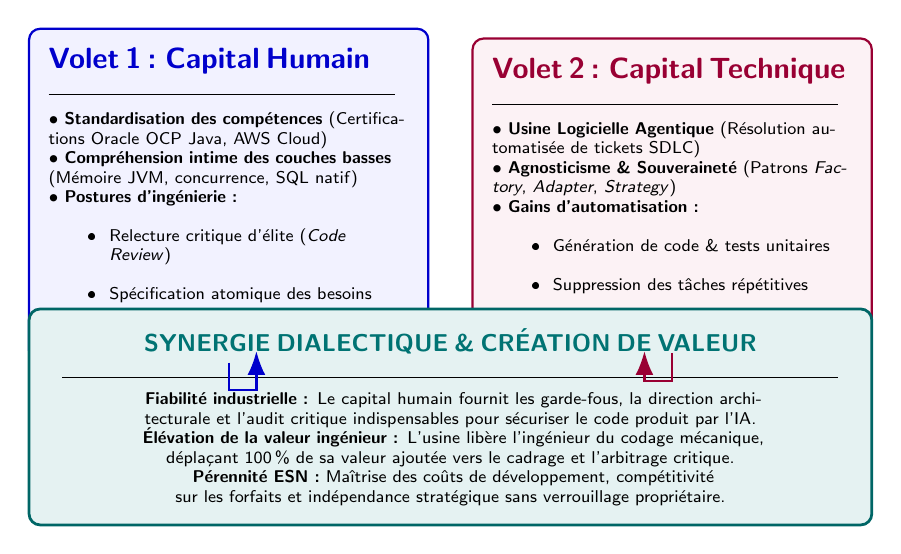
\begin{tikzpicture}[
    scale=0.88,
    transform shape,
    font=\sffamily\scriptsize,
    pillarbox/.style={draw=blue!80!black, fill=blue!5, rounded corners=4pt, inner sep=8pt, line width=0.8pt, text width=5.2cm},
    synergybox/.style={draw=teal!80!black, fill=teal!10, rounded corners=4pt, inner sep=8pt, line width=1.0pt, text width=11.6cm, align=center},
    arrowstyle/.style={-{Latex[length=3mm]}, thick, draw=blue!70!black}
]

    % Pilier 1 : Capital Humain
    \node[pillarbox] (humain) at (-3.2, 3.2) {
        \textbf{\large\color{blue!80!black} Volet 1 : Capital Humain}\\[3pt]
        \rule{5.0cm}{0.4pt}\\[4pt]
        $\bullet$ \textbf{Standardisation des compétences} (Certifications Oracle OCP Java, AWS Cloud)\\
        $\bullet$ \textbf{Compréhension intime des couches basses} (Mémoire JVM, concurrence, SQL natif)\\
        $\bullet$ \textbf{Postures d'ingénierie :}
        \begin{itemize}
            \item Relecture critique d'élite (\textit{Code Review})
            \item Spécification atomique des besoins
            \item Conception architecturale \& Sécurité
        \end{itemize}
    };

    % Pilier 2 : Capital Technique
    \node[pillarbox, draw=purple!80!black, fill=purple!5] (technique) at (3.2, 3.2) {
        \textbf{\large\color{purple!80!black} Volet 2 : Capital Technique}\\[3pt]
        \rule{5.0cm}{0.4pt}\\[4pt]
        $\bullet$ \textbf{Usine Logicielle Agentique} (Résolution automatisée de tickets SDLC)\\
        $\bullet$ \textbf{Agnosticisme \& Souveraineté} (Patrons \textit{Factory}, \textit{Adapter}, \textit{Strategy})\\
        $\bullet$ \textbf{Gains d'automatisation :}
        \begin{itemize}
            \item Génération de code \& tests unitaires
            \item Suppression des tâches répétitives
            \item Vélocité sur engagements au forfait
        \end{itemize}
    };

    % Nœud central : Synergie
    \node[synergybox] (synergie) at (0, 0) {
        \textbf{\normalsize\color{teal!90!black} SYNERGIE DIALECTIQUE \& CRÉATION DE VALEUR}\\[3pt]
        \rule{11.2cm}{0.4pt}\\[3pt]
        $\checkmark$ \textbf{Fiabilité industrielle :} Le capital humain fournit les garde-fous, la direction architecturale et l'audit critique indispensables pour sécuriser le code produit par l'IA.\\
        $\checkmark$ \textbf{Élévation de la valeur ingénieur :} L'usine libère l'ingénieur du codage mécanique, déplaçant 100\,\% de sa valeur ajoutée vers le cadrage et l'arbitrage critique.\\
        $\checkmark$ \textbf{Pérennité ESN :} Maîtrise des coûts de développement, compétitivité sur les forfaits et indépendance stratégique sans verrouillage propriétaire.
    };

    % Flèches
    \draw[arrowstyle, draw=blue!80!black] (humain.south) -- ++(0,-0.4) -| (-2.8, 0.95);
    \draw[arrowstyle, draw=purple!80!black] (technique.south) -- ++(0,-0.4) -| (2.8, 0.95);

\end{tikzpicture}
\caption{Modèle de synergie dialectique : l'interdépendance vertueuse entre capital humain certifié et usine logicielle agentique agnostique}
\label{fig:synergie_dialectique}
\end{figure}

\section{La stratégie d'ingénierie : Justification de la synergie entre formation continue et automatisation agentique}
\label{sec:strategie_ingenierie}

Loin de constituer deux initiatives déconnectées, la standardisation du capital humain (Volet 1) et l'industrialisation du capital technique (Volet 2) forment le cœur d'une stratégie d'ingénierie intégrée chez Oxyl. Face aux mutations profondes induites par l'intelligence artificielle générative dans l'industrie logicielle, cette stratégie répond à un impératif double : préparer l'entreprise aux futures pratiques du marché tout en garantissant un niveau de qualité irréprochable face aux exigences de ses clients grands comptes.

\subsection{Anticipation du marché : les projets internes comme banc d'essai industriel}
\label{subsec:anticipation_marche}

Le marché de la prestation de services numériques traverse une phase de transition asymétrique. D'un côté, les modèles d'intelligence artificielle agentique démontrent un potentiel de rupture pour le cycle de développement logiciel (SDLC) ; de l'autre, les grands comptes institutionnels (notamment dans la bancassurance et l'industrie) manifestent une frilosité légitime vis-à-vis de l'intégration directe de solutions d'IA au sein de leurs dépôts de code de production, freinés par des contraintes de confidentialité, de sécurité et de conformité réglementaire.

Dans ce contexte, la maîtrise de l'outillage IA constitue d'ores et déjà un facteur différenciant pour valoriser le profil des consultants en mission. Néanmoins, pour ne pas subir passivement les évolutions technologiques, Oxyl a fait le choix stratégique d'utiliser son pôle de R\&D et ses projets internes comme banc d'essai pour son usine logicielle agentique. Cette démarche proactive permet à l'entreprise d'éprouver, d'optimiser et de fiabiliser ses outils d'automatisation en conditions réelles, afin d'être immédiatement opérationnelle et force de proposition dès que les organisations avant-gardistes ouvriront leurs infrastructures à ces nouveaux paradigmes.

Par ailleurs, l'IA ne se limite pas à un outil de génération : elle agit comme un accélérateur cognitif majeur au service de la formation continue des ingénieurs, facilitant l'assimilation rapide de nouvelles stacks techniques et amplifiant la dynamique d'apprentissage.

\subsection{La transmission du savoir-faire : de l'expertise humaine aux garde-fous de l'usine}
\label{subsec:transmission_savoir_faire}

L'ordonnancement chronologique du stage — débutant par trois mois d'immersion technique intensive \textit{from scratch} sur \textit{NewroFactory} avant d'aborder les briques de l'usine logicielle — découle d'une nécessité technique fondamentale : un ingénieur ne peut piloter, auditer ou contraindre une chaîne de génération automatique sur des aspects qu'il ne maîtrise pas lui-même en profondeur.

Ce que le développeur assimile durant sa formation (règles de \textit{Clean Code}, architecture en couches, gestion fine des transactions et patrons de conception) constitue la matière première injectée dans l'usine logicielle :
\begin{itemize}
    \item \textbf{Le cadrage comportemental par les \textit{system prompts} :} l'expertise de l'ingénieur permet de formaliser les directives, les rôles spécialisés (\textit{personas}) et les contraintes de conception imposés aux agents lors des phases de planification et de rédaction ;
    \item \textbf{L'outillage de validation déterministe :} la rigueur méthodologique acquise permet de concevoir des scripts d'évaluation stricts (compilation rigoureuse, tests unitaires et d'intégration, analyse statique via SonarQube, vérification de types) servant de portes de qualité (\textit{quality gates}) incontournables avant toute proposition de modification.
\end{itemize}

À mesure que l'usine gagne en maturité et produit un code de plus en plus fiable, le temps consacré aux revues de code triviales diminue. Ce gain de productivité libère une charge cognitive précieuse, permettant à l'ingénieur d'élever sa posture professionnelle : il consacre désormais l'essentiel de son temps à la réflexion architecturale, à la modélisation du domaine métier et à la supervision stratégique des comportements de l'usine.

\subsection{Agnosticité et réassurance client : la garantie d'une ingénierie mature}
\label{subsec:agnosticite_reassurance}

Face aux réticences des directions informatiques clientes, la stratégie d'Oxyl repose sur un contrat de confiance fondé sur l'excellence démontrable de ses ingénieurs. Un consultant doté d'une solide discipline technique n'acceptera jamais qu'une chaîne automatisée produise des livrables inférieurs aux standards industriels en vigueur. L'exigence du capital humain sert ainsi de caution morale et technique à la production du capital automatisé.

Enfin, le choix d'une architecture résolument agnostique — découplée des fournisseurs de modèles de langage (LLMs) et des forges logicielles (GitLab, GitHub, Bitbucket) — constitue un marqueur d'ingénierie décisif. En génie logiciel, la capacité à généraliser et abstraire un processus n'intervient qu'après la preuve de son plein fonctionnement opérationnel. Démontrer une indépendance technologique totale prouve que l'usine logicielle dépasse le stade du prototype expérimental pour atteindre celui de produit industriel robuste. Ce découplage facilite l'adoption future chez les clients en leur permettant d'intégrer l'usine directement au sein de leur propre écosystème d'outils, sans friction ni remise en cause de leurs standards établis.

\bigskip
Ce rapport s'articule ainsi autour de la concrétisation de cette stratégie d'ingénierie à double détente :
\begin{itemize}
    \item Le \textbf{Chapitre~\ref{chap:quiz}} détaille la standardisation du capital humain à travers la conception et le développement de la plateforme de formation \textit{NewroFactory} (Volet~1) ;
    \item Les \textbf{Chapitres~\ref{chap:usine_ia}} et~\textbf{\ref{chap:infra_agnostique}} explorent l'industrialisation du capital technique, depuis l'état de l'art agentique jusqu'à la mise en œuvre de l'infrastructure logicielle agnostique (Volet~2) ;
    \item Enfin, le \textbf{Chapitre~\ref{chap:analyse_critique}} propose une analyse critique systémique de cette synergie, mesurant ses retombées industrielles, ses gains de productivité et ses limites éthiques.
\end{itemize}

\cleardoublepage

\chapter{La standardisation du capital humain (Volet 1 - Le Quiz)}
\label{chap:quiz}

\section{Analyse des besoins en montée en compétences : Le rôle du socle Java/JEE dans la qualité logicielle}
\label{sec:analyse_besoins}

La standardisation du capital humain au sein d'une Entreprise de Services du Numérique (ESN) repose sur une adéquation stricte entre la maîtrise des fondamentaux théoriques et les exigences opérationnelles des clients. Cette section explicite les facteurs de marché et les impératifs d'ingénierie ayant conduit à la définition du socle Java/JEE, détaille les limites de l'outillage existant et formalise le cahier des charges fonctionnel de la plateforme \textit{NewroFactory}.

\subsection{Évolution du marché et impératif de certification industrielle}
\label{subsec:evolution_marche_certifications}

Dans les premières phases d'expansion du secteur du numérique, la tension extrême sur le marché du recrutement conduisait les entreprises à embaucher des profils d'ingénieurs et de développeurs sans exiger de garanties formelles préalables. L'accès rapide aux projets primait sur la vérification systématique et objective des acquis techniques.

Aujourd'hui, le niveau d'exigence des donneurs d'ordre s'est considérablement accru. Les clients attendent des ESN des garanties tangibles sur la qualification de leurs consultants afin de sécuriser des projets d'envergure, soumis à de fortes contraintes de maintenabilité et de scalabilité. Pour répondre à cette exigence de réassurance, Oxyl a instauré un passage obligatoire de certifications industrielles reconnues dès la phase d'intégration des nouveaux collaborateurs :
\begin{itemize}
    \item \textbf{Oracle Certified Associate (OCA) \& Oracle Certified Professional (OCP) Java SE :} validation formelle de la maîtrise approfondie du langage Java, de sa syntaxe, de la gestion mémoire, du modèle de concurrence et des patrons de conception objet (certificat officiel OCA reproduit en Figure~\ref{fig:certificat_oca}, Annexe~\ref{annexe:certifications}) ;
    \item \textbf{AWS Certified Cloud Practitioner :} certification attestant de la compréhension des architectures distribuées, des services cloud fondamentaux, de la sécurité et des modèles de déploiement industriels (accréditation officielle reproduite en Figure~\ref{fig:certificat_aws}, Annexe~\ref{annexe:certifications}).
\end{itemize}

L'obtention de ces certifications ne constitue pas un simple label commercial, mais un jalon garantissant qu'un socle d'excellence homogène est partagé par l'ensemble des consultants avant leur projection en mission.

L'impact quantitatif de la plateforme \textbf{MyNewroFactory (MNF)} sur cette démarche est spectaculaire :
\begin{itemize}
    \item \textbf{Avant MNF :} le cycle de révision et d'assimilation mobilisait en moyenne \textbf{$3$~mois} pour l'obtention de l'OCA et près d'\textbf{$1$~an} pour l'OCP ;
    \item \textbf{Avec MNF :} la préparation de l'OCA est réduite à \textbf{moins d'un mois} (délai divisé par trois, $\div 3$) et celle de l'OCP à environ \textbf{$6$~mois} (délai réduit de moitié, $\div 2$).
\end{itemize}

Cette accélération mesurable sécurise le modèle économique d'Oxyl en réduisant drastiquement les délais d'intercontrat non facturés et en permettant un staffing client ultra-rapide sur des missions à haute valeur ajoutée. De surcroît, la plateforme MNF s'inscrit au cœur du cycle de vie complet du consultant : elle est activement exploitée pour la formation continue des profils confirmés et sert d'outil d'entraînement intensif pour préparer les entretiens techniques de qualification client.

\subsection{Le socle Java et la programmation orientée objet comme vecteurs de qualité}
\label{subsec:role_socle_java_poo}

Le choix d'asseoir la formation initiale sur l'écosystème Java/JEE répond à des critères d'ingénierie logicielle rigoureux :
\begin{enumerate}
    \item \textbf{Rigueur et expressivité de la Programmation Orientée Objet (POO) :} En tant que langage fortement typé et orienté objet, Java impose une discipline de modélisation stricte. Ses mécanismes fondamentaux (encapsulation, polymorphisme, héritage, interfaces, généricité) permettent de transcrire fidèlement les règles et les relations des domaines métiers complexes. Cette fidélité de modélisation est indispensable à la conception d'architectures web robustes et modulaires ;
    \item \textbf{Gestion avancée de la concurrence et du cycle de vie :} La maîtrise des particularités fines de la JVM (mécanismes du \textit{Garbage Collector}, collections thread-safe, flux réactifs) est essentielle pour concevoir des applications résilientes sous forte charge et prévenir les régressions de performance ;
    \item \textbf{Base fondamentale pour l'écosystème d'entreprise :} La maîtrise du langage sous-jacent (Java SE) constitue le prérequis indispensable pour appréhender avec discernement les frameworks d'entreprise tels que Spring Boot, Spring Security et Hibernate, évitant ainsi le piège du « développement par copier-coller » ou l'usage magique d'annotations sans compréhension des mécanismes sous-jacents.
\end{enumerate}

\subsection{Limites de l'outillage existant et identification des besoins}
\label{subsec:limites_outillage_besoins}

Bien qu'un outil interne d'entraînement aux certifications ait été utilisé par le passé au sein d'Oxyl, les retours d'expérience ont mis en lumière plusieurs lacunes structurelles :
\begin{itemize}
    \item \textbf{Carence d'analyses et de métriques granulaires :} Les versions précédentes ne proposaient qu'un score brut en fin de série, sans capacité de décomposer les résultats par domaine de connaissances. Les stagiaires ne disposaient d'aucune visibilité quantifiée sur leurs points faibles spécifiques au sein d'un même programme d'examen ;
    \item \textbf{Absence de suivi pédagogique centralisé :} Les tuteurs et encadrants ne disposaient pas d'une vue d'ensemble consolidée pour évaluer la trajectoire de montée en compétences d'une promotion entière ni pour adapter leur accompagnement aux difficultés récurrentes ;
    \item \textbf{Manque d'interactivité et d'outils d'approfondissement :} En mode entraînement, la découverte d'une erreur n'était pas couplée à des mécanismes d'exploration complémentaires permettant à l'apprenant de creuser la notion théorique au-delà du corrigé statique.
\end{itemize}

\subsection{Cahier des charges fonctionnel et innovations de la plateforme}
\label{subsec:cahier_des_charges_fonctionnel}

Pour combler ces lacunes, le cahier des charges de \textit{NewroFactory} s'est articulé autour de deux axes majeurs : l'autonomie analytique de l'apprenant et le pilotage fin par l'encadrement.

\subsubsection{Besoins apprenants : Visualisation analytique et synergie avec les LLM}
Pour maximiser l'efficacité de l'entraînement, la plateforme devait intégrer :
\begin{itemize}
    \item \textbf{Un tableau de bord de diagnostic des compétences :} Présentation claire et hiérarchisée des pourcentages de réussite par chapitre et par série, complétée par le taux de complétion des questions disponibles par notion. Cette double métrique permet au stagiaire d'identifier immédiatement les chapitres sous-travaillés ou mal assimilés ;
    \item \textbf{Deux modes d'entraînement complémentaires :} Un mode \textit{Entraînement} interactif (feedback immédiat et explications détaillées pour chaque proposition) et un mode \textit{Examen blanc} (chronométré, tirage étanche, conditions réelles) ;
    \item \textbf{Export structuré JSON pour approfondissement via LLM :} Innovation clé développée sur la plateforme, l'interface de correction en mode entraînement propose un bouton d'exportation instantané au format JSON (illustré en Figure~\ref{fig:ui_question_test}). Ce bouton copie dans le presse-papier l'intégralité du contexte de la question (énoncé, code snippet, propositions, statut de validation, explications). L'apprenant peut ainsi soumettre directement ces métadonnées à un grand modèle de langage (LLM) afin d'obtenir des explications interactives, des contre-exemples ou des variantes pédagogiques sur la notion précise abordée.
\end{itemize}

\begin{figure}[htbp]
    \centering
    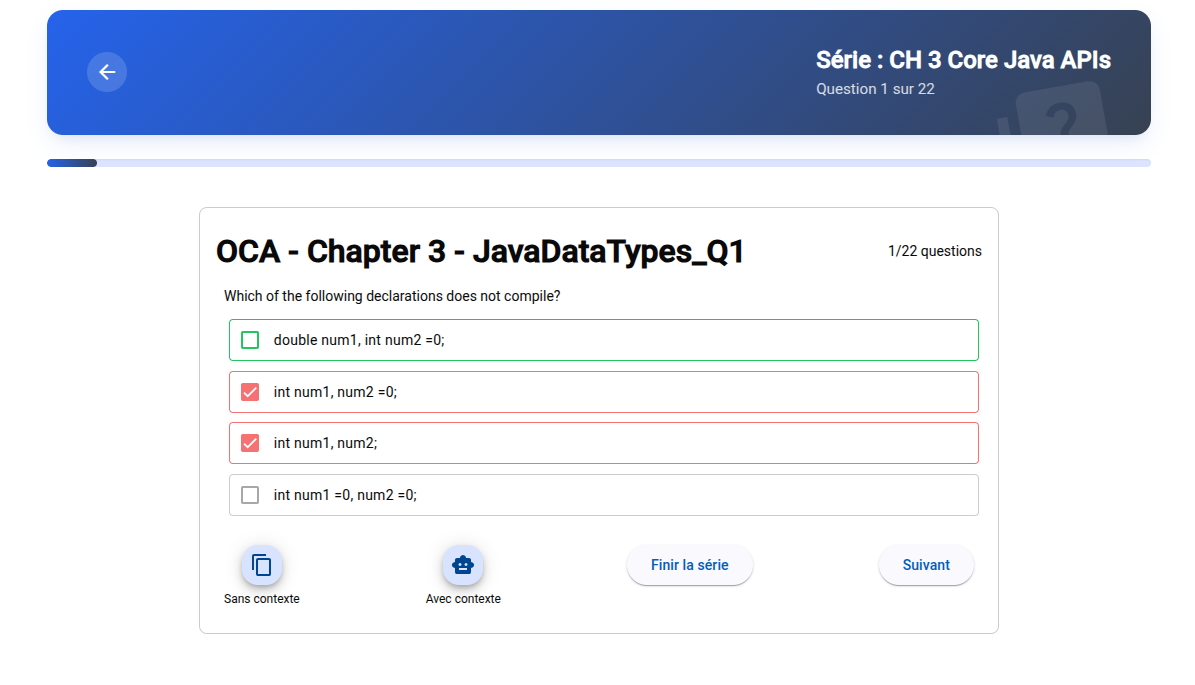
\includegraphics[width=0.92\textwidth]{figures/quiz_question_feedback_llm.png}
    \caption{Interface de passation de test en mode entraînement : validation visuelle immédiate des réponses et boutons d'exportation contextuelle pour LLM (« Sans contexte » et « Avec contexte »)}
    \label{fig:ui_question_test}
\end{figure}

\begin{figure}[htbp]
    \centering
    
\includegraphics[width=0.72\textwidth]{figures/quiz_serie_terminee.png}
    \caption{Écran de restitution finale à l'issue d'une série d'entraînement : score obtenu, taux de complétion et diagnostic de révision}
    \label{fig:ui_serie_terminee}
\end{figure}

\subsubsection{Besoins encadrants : Gouvernance et assignation ciblée}
Du côté de l'administration et du tutorat technique, les exigences comprenaient :
\begin{itemize}
    \item \textbf{Gestion des identités et des rôles :} Distinction stricte entre les profils stagiaires et formateurs/administrateurs ;
    \item \textbf{Supervision globale des promotions :} Tableau de bord analytique transverse offrant aux tuteurs une visibilité sur les statistiques agrégées et individuelles de l'ensemble des stagiaires ;
    \item \textbf{Création et assignation de séries personnalisées :} Capacité pour l'encadrant de composer des séries d'évaluation sur-mesure et de les assigner directement au tableau de bord de stagiaires ciblés pour remédier à des lacunes précises ;
    \item \textbf{Administration dynamique du référentiel pédagogique :} Outils complets de gestion (CRUD) des chapitres hiérarchiques, des questions, des propositions et de leurs explications associées.
\end{itemize}

\begin{figure}[htbp]
\centering
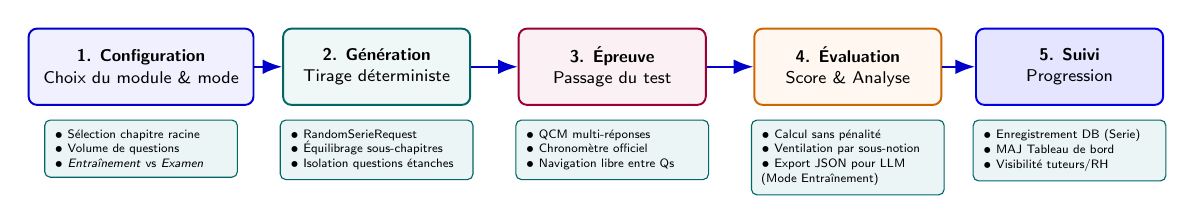
\begin{tikzpicture}[
    scale=0.88,
    transform shape,
    font=\sffamily\scriptsize,
    stepbox/.style={draw=blue!80!black, fill=blue!6, rounded corners=3pt, align=center, inner sep=6pt, line width=0.7pt, minimum width=2.7cm, minimum height=1.1cm},
    decision/.style={draw=orange!80!black, fill=orange!8, diamond, aspect=1.8, align=center, inner sep=3pt, line width=0.7pt, font=\sffamily\bfseries\tiny},
    actionbox/.style={draw=teal!80!black, fill=teal!8, rounded corners=2pt, align=left, inner sep=4pt, font=\sffamily\tiny, text width=2.5cm},
    flowarrow/.style={-{Latex[length=2.5mm]}, thick, draw=blue!80!black}
]

    % Étape 1 : Configuration
    \node[stepbox] (step1) at (0, 0) {\textbf{1. Configuration}\\[1pt]Choix du module \& mode};
    \node[actionbox, below=0.2cm of step1] (act1) {
        $\bullet$ Sélection chapitre racine\\
        $\bullet$ Volume de questions\\
        $\bullet$ \textit{Entraînement} vs \textit{Examen}
    };

    % Étape 2 : Tirage
    \node[stepbox, fill=teal!6, draw=teal!80!black] (step2) at (3.4, 0) {\textbf{2. Génération}\\[1pt]Tirage déterministe};
    \node[actionbox, below=0.2cm of step2] (act2) {
        $\bullet$ \code{RandomSerieRequest}\\
        $\bullet$ Équilibrage sous-chapitres\\
        $\bullet$ Isolation questions étanches
    };

    % Étape 3 : Déroulement
    \node[stepbox, fill=purple!6, draw=purple!80!black] (step3) at (6.8, 0) {\textbf{3. Épreuve}\\[1pt]Passage du test};
    \node[actionbox, below=0.2cm of step3] (act3) {
        $\bullet$ QCM multi-réponses\\
        $\bullet$ Chronomètre officiel\\
        $\bullet$ Navigation libre entre Qs
    };

    % Étape 4 : Évaluation
    \node[stepbox, fill=orange!6, draw=orange!80!black] (step4) at (10.2, 0) {\textbf{4. Évaluation}\\[1pt]Score \& Analyse};
    \node[actionbox, below=0.2cm of step4] (act4) {
        $\bullet$ Calcul sans pénalité\\
        $\bullet$ Ventilation par sous-notion\\
        $\bullet$ Export JSON pour LLM (Mode Entraînement)
    };

    % Étape 5 : Historisation
    \node[stepbox, fill=blue!10, draw=blue!90!black] (step5) at (13.4, 0) {\textbf{5. Suivi}\\[1pt]Progression};
    \node[actionbox, below=0.2cm of step5] (act5) {
        $\bullet$ Enregistrement DB (\code{Serie})\\
        $\bullet$ MAJ Tableau de bord\\
        $\bullet$ Visibilité tuteurs/RH
    };

    % Flèches
    \draw[flowarrow] (step1) -- (step2);
    \draw[flowarrow] (step2) -- (step3);
    \draw[flowarrow] (step3) -- (step4);
    \draw[flowarrow] (step4) -- (step5);

\end{tikzpicture}
\caption{Workflow fonctionnel du parcours apprenant sur la plateforme NewroFactory : de la configuration de l'épreuve à la restitution analytique}
\label{fig:workflow_parcours_quiz}
\end{figure}

\subsection{Objectifs d'ingénierie et exigences implicites}
\label{subsec:objectifs_contraintes}

Le projet s'est vu confier une consigne fondatrice : \textbf{convaincre les parties prenantes et les équipes commerciales} de la pertinence de la solution en démontrant qu'elle répondait avec excellence aux standards industriels actuels.

Cette orientation imposait de facto des contraintes de réalisation implicites mais déterminantes :
\begin{itemize}
    \item \textbf{Excellence ergonomique et design moderne :} Concevoir une interface soignée, responsive et intuitive (développée sous Angular), surpassant les outils internes traditionnels pour susciter une adhésion immédiate des utilisateurs ;
    \item \textbf{Robustesse et performance logicielle :} Assurer une réactivité instantanée des interactions et garantir l'étanchéité des sessions d'examen via une architecture backend Spring Core/Boot découplée ;
    \item \textbf{Sécurité et intégrité :} Mettre en œuvre une gestion robuste des sessions et des droits d'accès pour préserver la confidentialité des évaluations et l'intégrité des données d'examen.
\end{itemize}

\section{Ingénierie de la plateforme : Conception d'un système de contrôle qualité des connaissances}
\label{sec:conception_systeme}

Pour concrétiser la politique d'excellence technique d'Oxyl et standardiser le capital humain, nous avons conçu et développé \textit{NewroFactory}, une plateforme web sur-mesure d'évaluation et de validation des compétences. Ce système vise un double objectif pédagogique et opérationnel : offrir aux apprenants un environnement d'auto-évaluation interactif aligné sur les référentiels officiels de l'industrie (tels qu'Oracle Java SE OCP et AWS Cloud Practitioner), tout en fournissant aux encadrants techniques un instrument de mesure quantitatif et objectif de la progression des stagiaires.

\subsection{Modélisation du domaine et structuration arborescente des connaissances}
\label{subsec:modelisation_domaine}

La première exigence d'ingénierie a consisté à concevoir un modèle de données capable d'épouser fidèlement la granularité des référentiels pédagogiques officiels sans introduire de rigidité structurelle.

\subsubsection{Hiérarchisation des chapitres par chemin matérialisé (\textit{Materialized Path})}
Les programmes d'examens professionnels s'organisent selon une hiérarchie stricte en modules, chapitres et sous-notions (par exemple : \textit{Java Concurrency} $\rightarrow$ \textit{Thread-Safe Collections} $\rightarrow$ \textit{ConcurrentHashMap}). Pour représenter cette arborescence parent-enfant en base de données relationnelle sans subir les limites de performance des requêtes récursives profondes (\textit{Common Table Expressions} ou jointures récursives multiples), nous avons mis en œuvre le patron de conception par \textbf{chemin matérialisé} (\textit{Materialized Path}).

Dans l'entité \texttt{ChapterEntity}, chaque nœud stocke explicitement la chaîne hiérarchique de ses ascendants dans un champ \texttt{parentPath} (ex. \texttt{"/1/4/"}) :

\begin{lstlisting}[language=java, caption={Modélisation de l'entité ChapterEntity avec chemin matérialisé et suppression logique}, label={lst:chapterEntity}]
@Entity
@Table(name = "chapter", uniqueConstraints = @UniqueConstraint(columnNames = {"name", "parent_path"}))
@SoftDelete(columnName = "is_deleted")
public class ChapterEntity {

    @Id
    @GeneratedValue(strategy = GenerationType.IDENTITY)
    private Long id;

    @Column(name = "name", nullable = false)
    private String name;

    @Column(name = "parent_path")
    private String parentPath;

    @Formula("is_deleted")
    private Boolean isDeleted;

    // Getters, Setters et methodes metier
}
\end{lstlisting}

Cette modélisation permet d'effectuer des opérations ensemblistes hautement performantes :
\begin{itemize}
    \item L'extraction de l'ensemble des sous-chapitres descendants d'un nœud s'effectue par un simple filtre de préfixe SQL (\code{parent_path LIKE '/1/4/%'}) ;
    \item L'agrégation et le décompte global des questions rattachées à un module complet et à l'ensemble de ses sous-arborescences s'exécutent en une unique passe indexée (\code{countQuestionsByChapterIdsAndChildren}) ;
    \item L'intégrité de l'arbre est protégée par une contrainte d'unicité composite sur \texttt{(name, parent\_path)} et par la mise en œuvre du mécanisme de suppression logique (\textit{Soft Delete}) via l'annotation Hibernate \code{@SoftDelete}.
\end{itemize}

La Figure~\ref{fig:ui_arborescence_chapitres} illustre la restitution dynamique de cette arborescence dans l'interface d'administration, où les chapitres, sous-chapitres et le nombre de questions rattachées sont consolidés à chaque niveau.

\begin{figure}[htbp]
    \centering
    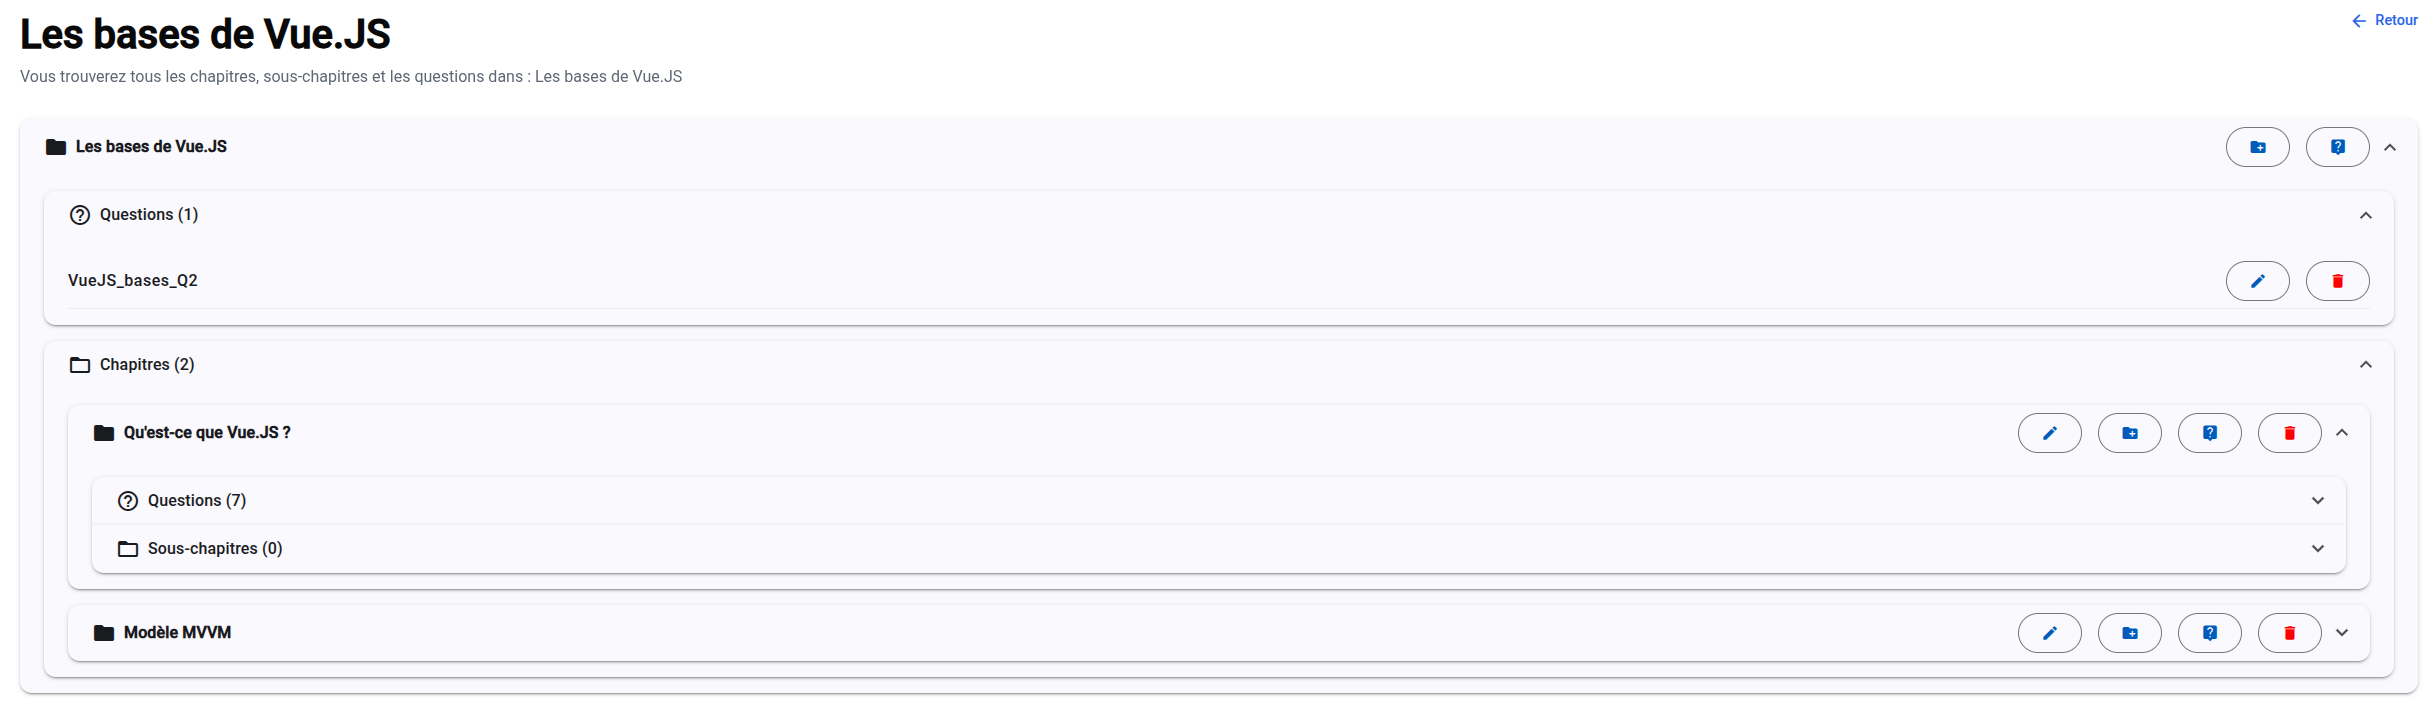
\includegraphics[width=0.92\textwidth]{figures/quiz_arborescence_chapitres.png}
    \caption{Interface de gestion hiérarchique des compétences et chapitres : structuration arborescente dynamique exploitant le patron \textit{Materialized Path}}
    \label{fig:ui_arborescence_chapitres}
\end{figure}

\subsubsection{Modélisation des questions et étanchéité des examens blancs}
Les questions sont modélisées sous forme de Questionnaires à Choix Multiples (QCM) sans pénalité de points négatifs, conformes aux modalités réelles des certifications Oracle et AWS. Chaque question est rattachée à un chapitre spécifique et comporte un ensemble de propositions dont une ou plusieurs peuvent être valides.

Un enjeu méthodologique central résidait dans l'évitement du biais de mémorisation passive. Si les stagiaires s'entraînent quotidiennement sur l'ensemble de la base de questions, les examens blancs hebdomadaires du vendredi perdent leur valeur diagnostique. Pour garantir une étanchéité stricte :
\begin{enumerate}
    \item Les questions réservées aux examens officiels sont isolées dans un chapitre racine dédié (\textit{Examen Blanc}) ;
    \item Les sessions d'entraînement permettent au stagiaire de sélectionner librement le chapitre cible ainsi que le volume de questions souhaité, lesquelles sont alors sélectionnées aléatoirement au sein du vivier d'entraînement ;
    \item Les examens blancs imposent un gabarit rigoureusement identique aux conditions réelles de passage (même volumétrie intégrale et tirage exclusif parmi les questions étanches).
\end{enumerate}

\subsubsection{Modes d'évaluation : Entraînement vs Examen}
La plateforme intègre deux modes d'évaluation distincts :
\begin{itemize}
    \item \textbf{Le mode Entraînement (formatif) :} favorise l'apprentissage itératif en fournissant une correction immédiate dès la validation de chaque question, accompagnée d'une explication technique détaillée justifiant pourquoi les alternatives erronées ont été écartées ;
    \item \textbf{Le mode Examen (sommatif) :} simule l'épreuve officielle. Aucun feedback ni indice n'est retourné pendant le déroulement de la série. Le stagiaire ne découvre son score global qu'à l'issue de la soumission définitive, sans affichage des explications par question afin d'éviter toute fixation de réponses lors des sessions ultérieures.
\end{itemize}

Les Figures~\ref{fig:ui_assign_step1} et~\ref{fig:ui_assign_step2} illustrent le parcours de configuration et d'assignation d'une série personnalisée par l'encadrant ou l'apprenant.

\begin{figure}[htbp]
    \centering
    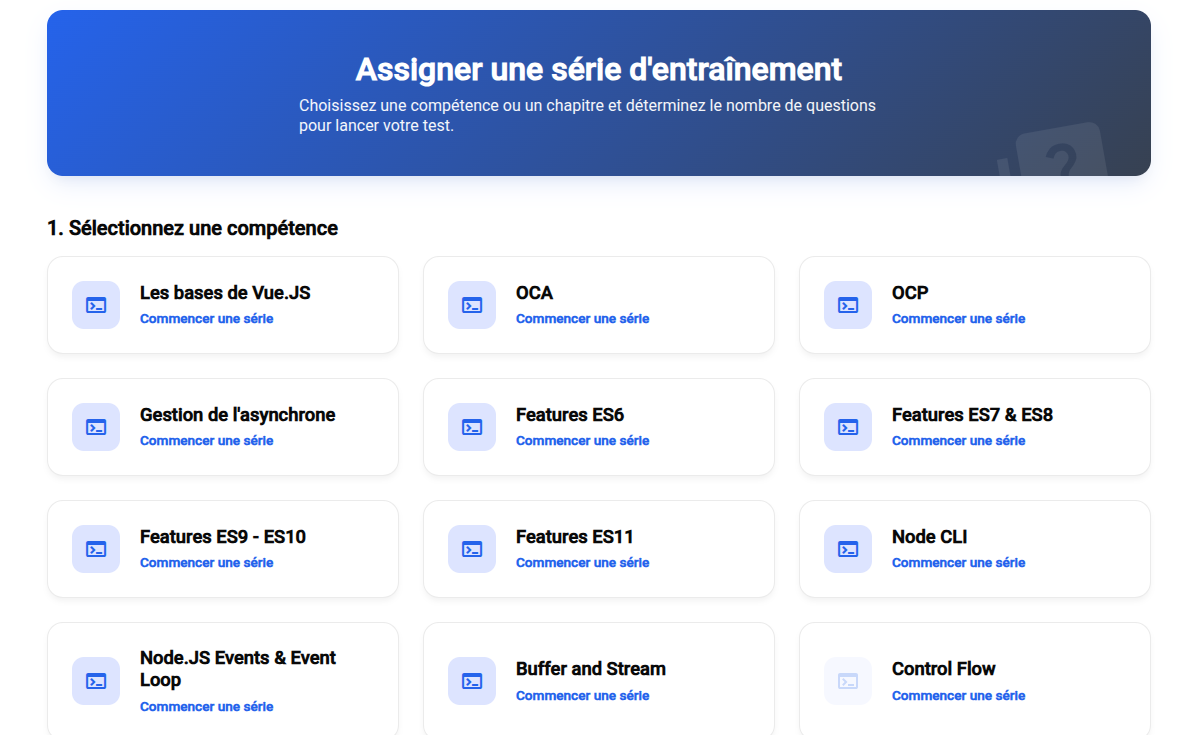
\includegraphics[width=0.88\textwidth]{figures/quiz_assign_serie_step1.png}
    \caption{Étape 1 de configuration d'une série : sélection du module de certification cible (Vue.js, Java OCA/OCP, Node CLI, Spring)}
    \label{fig:ui_assign_step1}
\end{figure}

\begin{figure}[htbp]
    \centering
    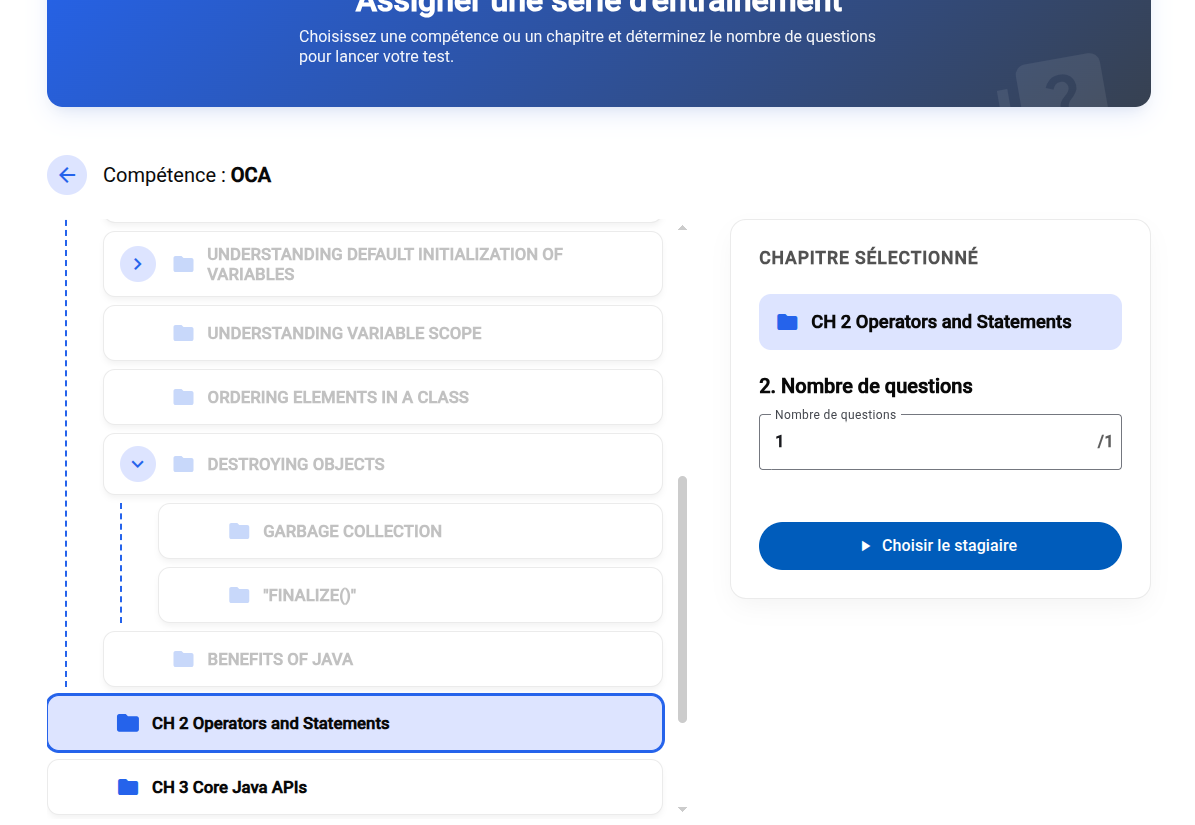
\includegraphics[width=0.88\textwidth]{figures/quiz_assign_serie_step2.png}
    \caption{Étape 2 de configuration d'une série : sélection granulaire du sous-chapitre dans l'arborescence et définition du volume de questions}
    \label{fig:ui_assign_step2}
\end{figure}

\subsection{Architecture logicielle backend et services RESTful}
\label{subsec:architecture_backend_spring}

Le backend de \textit{NewroFactory} a été développé en Java avec le framework Spring, selon une architecture en couches étanches respectant les principes de responsabilité unique (\textit{Single Responsibility Principle} - SRP) et d'inversion de dépendances (illustrée en Figure~\ref{fig:architecture_globale_quiz}).

\begin{figure}[htbp]
\centering
\begin{tikzpicture}[
    scale=0.88,
    transform shape,
    font=\sffamily\scriptsize,
    tierbox/.style={draw=blue!80!black, fill=blue!4, rounded corners=4pt, inner sep=6pt, line width=0.8pt},
    compbox/.style={draw=blue!70!black, fill=white, rounded corners=2pt, align=center, inner sep=4pt, line width=0.6pt, font=\sffamily\scriptsize},
    busarrow/.style={{Latex[length=2.5mm]}-{Latex[length=2.5mm]}, thick, draw=blue!80!black}
]

    % TIER 1 : FRONTEND
    \node[tierbox, fill=teal!4, draw=teal!80!black, text width=13.0cm] (tier_front) at (0, 4.2) {
        \textbf{\color{teal!80!black}\normalsize TIER 1 : Client Single Page Application (Angular 17)}\\[3pt]
        \begin{tikzpicture}[node distance=0.4cm]
            \node[compbox, fill=teal!10, draw=teal!70!black] (c1) at (-4.2, 0) {\textbf{Components UI}\\Quiz, Dashboard, Admin};
            \node[compbox, fill=teal!10, draw=teal!70!black] (c2) at (-0.3, 0) {\textbf{Services TypeScript}\\State Management, Observables RxJS};
            \node[compbox, fill=teal!10, draw=teal!70!black] (c3) at (3.8, 0) {\textbf{HTTP Interceptor}\\Gestion Token JWT \& Erreurs};
        \end{tikzpicture}
    };

    % TIER 2 : BACKEND SPRING
    \node[tierbox, text width=13.0cm] (tier_back) at (0, 1.2) {
        \textbf{\color{blue!80!black}\normalsize TIER 2 : API REST Backend (Java / Spring Framework)}\\[3pt]
        \begin{tikzpicture}
            \node[compbox, fill=blue!10, text width=3.4cm] (b1) at (-4.2, 0) {\textbf{Couche Présentation}\\\code{ChapterController}\\\code{SerieController}\\\code{UserController}};
            \node[compbox, fill=purple!10, draw=purple!70!black, text width=3.8cm] (b2) at (0, 0) {\textbf{Couche Métier / Services}\\\code{SerieService} (Tirage aléatoire)\\\code{ChapterService} (Materialized Path)\\\code{ScoreCalculatorService}};
            \node[compbox, fill=blue!10, text width=3.4cm] (b3) at (4.2, 0) {\textbf{Couche Persistance}\\\code{ChapterRepository}\\\code{SerieRepository}\\\code{UserRepository}};
            \draw[-{Latex}, thick, draw=blue!60!black] (b1) -- (b2);
            \draw[-{Latex}, thick, draw=blue!60!black] (b2) -- (b3);
        \end{tikzpicture}\\[3pt]
        \centering\textit{\tiny Transverse : Spring Security (Filtre JWT) $\cdot$ Spring AOP (\code{LoggingAspect}, traduction d'exceptions DataAccessException)}
    };

    % TIER 3 : DATABASE
    \node[tierbox, fill=orange!4, draw=orange!80!black, text width=13.0cm] (tier_db) at (0, -1.6) {
        \textbf{\color{orange!80!black}\normalsize TIER 3 : Couche de Persistance \& Base de Données}\\[3pt]
        \begin{tikzpicture}
            \node[compbox, fill=orange!10, draw=orange!70!black, text width=5.5cm] (db1) at (-3.2, 0) {\textbf{Schéma Relationnel PostgreSQL / H2}\\Tables \code{chapter}, \code{question}, \code{answer}, \code{serie}, \code{user}};
            \node[compbox, fill=orange!10, draw=orange!70!black, text width=5.5cm] (db2) at (3.2, 0) {\textbf{Indexation \& Requêtes Hiérarchiques}\\Index sur \code{parent_path} (Materialized Path) \& Soft Delete};
        \end{tikzpicture}
    };

    % Connecteurs entre tiers
    \draw[busarrow, draw=teal!80!black] (tier_front) -- node[right, font=\sffamily\tiny\bfseries, text=teal!80!black] {Échanges RESTful (JSON) / En-tête Authorization: Bearer JWT} (tier_back);
    \draw[busarrow, draw=orange!80!black] (tier_back) -- node[right, font=\sffamily\tiny\bfseries, text=orange!80!black] {Spring Data JPA / Hibernate / Pool de connexions HikariCP} (tier_db);

\end{tikzpicture}
\caption{Architecture globale 3-tiers découplée de la plateforme NewroFactory (Angular, Spring Core REST et PostgreSQL)}
\label{fig:architecture_globale_quiz}
\end{figure}

\subsubsection{Découpage en couches et exposition des API}
L'architecture sépare rigoureusement la persistance, le domaine métier et l'exposition REST :
\begin{itemize}
    \item \textbf{Couche Présentation / Contrôleurs (\code{web.rest}) :} les points d'entrée tels que \code{ChapterController}, \code{SerieController} et \code{UserController} valident les requêtes entrantes (via Jakarta Validation et des validateurs personnalisés comme \code{StartDateBeforeEndDateValidator}), invoquent les services métiers et retournent des objets de transfert typés (\textit{DTOs}) ;
    \item \textbf{Couche Métier / Services (\code{service}) :} orchestre la logique d'évaluation, l'assemblage dynamique des séries aléatoires (\code{RandomSerieRequest}), le calcul des taux de réussite et la gestion des utilisateurs ;
    \item \textbf{Couche Persistance (\code{persistence}) :} s'appuie sur Spring Data JPA et Hibernate pour abstraire l'accès aux tables relationnelles MySQL via des interfaces de dépôts typées (\code{ChapterRepository}, \code{SerieRepository}, \code{SerieReponseRepository}).
\end{itemize}

\subsubsection{Observabilité et découplage transversal par Spring AOP}
Dans une application d'entreprise, la journalisation (\textit{logging}) et la gestion des erreurs ne doivent pas polluer la logique métier. Pour garantir une observabilité exhaustive et standardisée, nous avons mis en place une programmation orientée aspect (\textit{Aspect-Oriented Programming} - AOP) via le composant \code{LoggingAspect}.

\begin{lstlisting}[language=java, caption={Aspect transverse de logging et traduction des exceptions de persistance}, label={lst:loggingAspect}]
@Aspect
@Component
public class LoggingAspect {

    @Pointcut("execution(public * com.oxyl.newrofactory.service.*.*(..)) || "
            + "execution(public * com.oxyl.newrofactory.persistence.*.*(..)) || "
            + "execution(public * com.oxyl.newrofactory.web.*.*(..))")
    public void allLayersMethods() {}

    @Before("allLayersMethods()")
    public void logBefore(JoinPoint jp) {
        getLogger(jp).info("-> Appel de : {}.{}",
                jp.getTarget().getClass().getSimpleName(), jp.getSignature().getName());
    }

    @AfterReturning(pointcut = "allLayersMethods()", returning = "result")
    public void logAfterReturning(JoinPoint jp, Object result) {
        getLogger(jp).info("<- Retour de : {} -> {}",
                jp.getSignature().getName(), result);
    }

    @Pointcut("within(com.oxyl.newrofactory.persistence..*)")
    public void persistenceMethods() {}

    @AfterThrowing(pointcut = "persistenceMethods()", throwing = "exception")
    public void translateDataAccessException(JoinPoint jp, DataAccessException exception) {
        Logger logger = getLogger(jp);
        String className = jp.getTarget().getClass().getSimpleName();
        String methodName = jp.getSignature().getName();
        if (exception instanceof EmptyResultDataAccessException) {
            logger.warn("! [FONCTIONNEL] Element non trouve dans {}.{}() : {}", 
                    className, methodName, exception.getMessage());
        } else {
            logger.error("!! [CRITIQUE] Erreur SQL/Base de donnees dans {}.{}() : {}", 
                    className, methodName, exception.getMessage());
        }
    }
}
\end{lstlisting}

Cet aspect intercepte automatiquement chaque transition inter-couches à l'entrée et à la sortie des méthodes, mesure les flux et assure une discrimination fine entre les anomalies fonctionnelles (ex. entité introuvable notifiée en avertissement) et les défaillances critiques d'infrastructure (erreurs SQL journalisées au niveau \code{ERROR}).

\subsubsection{Moteur d'analytics et consolidation des statistiques}
Pour offrir une vue claire sur l'acquisition des compétences, le système consolide deux niveaux de métriques :
\begin{itemize}
    \item \textbf{Le score par série :} calculé à la fin de chaque questionnaire pour évaluer la performance ponctuelle sur un tirage donné ;
    \item \textbf{Le score agrégé par chapitre (\code{ChapterStat}) :} calculé à partir de l'historique complet des réponses d'un stagiaire, permettant d'identifier immédiatement les chapitres maîtrisés et les points de vulnérabilité conceptuelle.
\end{itemize}
Tandis que le stagiaire accède à son tableau de bord personnel, l'encadrant technique dispose d'un endpoint d'administration dédié (\code{/api/chapters/root/withStat/user/{userId}}) lui permettant de consulter les métriques individuelles de chaque collaborateur pour adapter son suivi pédagogique.

\subsection{Gouvernance des accès, Sécurité et Interopérabilité Front/Back}
\label{subsec:securite_cors}

En tant qu'outil interne destiné à une ESN, la gouvernance des identités et la sécurité des échanges constituent un pilier central de l'architecture.

\subsubsection{Gestion des sessions et création déléguée des comptes}
Afin de préserver la confidentialité des contenus et de garantir le rattachement hiérarchique des métriques, l'auto-inscription publique a été proscrite. La création de compte est exclusivement réservée aux encadrants et administrateurs (\code{ROLE_ADMIN}). Lorsqu'un encadrant crée le profil d'un stagiaire, ce dernier est explicitement rattaché à sa promotion dans le système (illustré en Figure~\ref{fig:ui_admin_users} et Figure~\ref{fig:ui_modal_edit_user}). Lors de sa première connexion avec ses identifiants temporaires, le stagiaire est invité à réinitialiser son mot de passe via un composant dédié (\code{update-password}), ce qui active l'historisation de ses statistiques sous la supervision de son tuteur.

\begin{figure}[htbp]
    \centering
    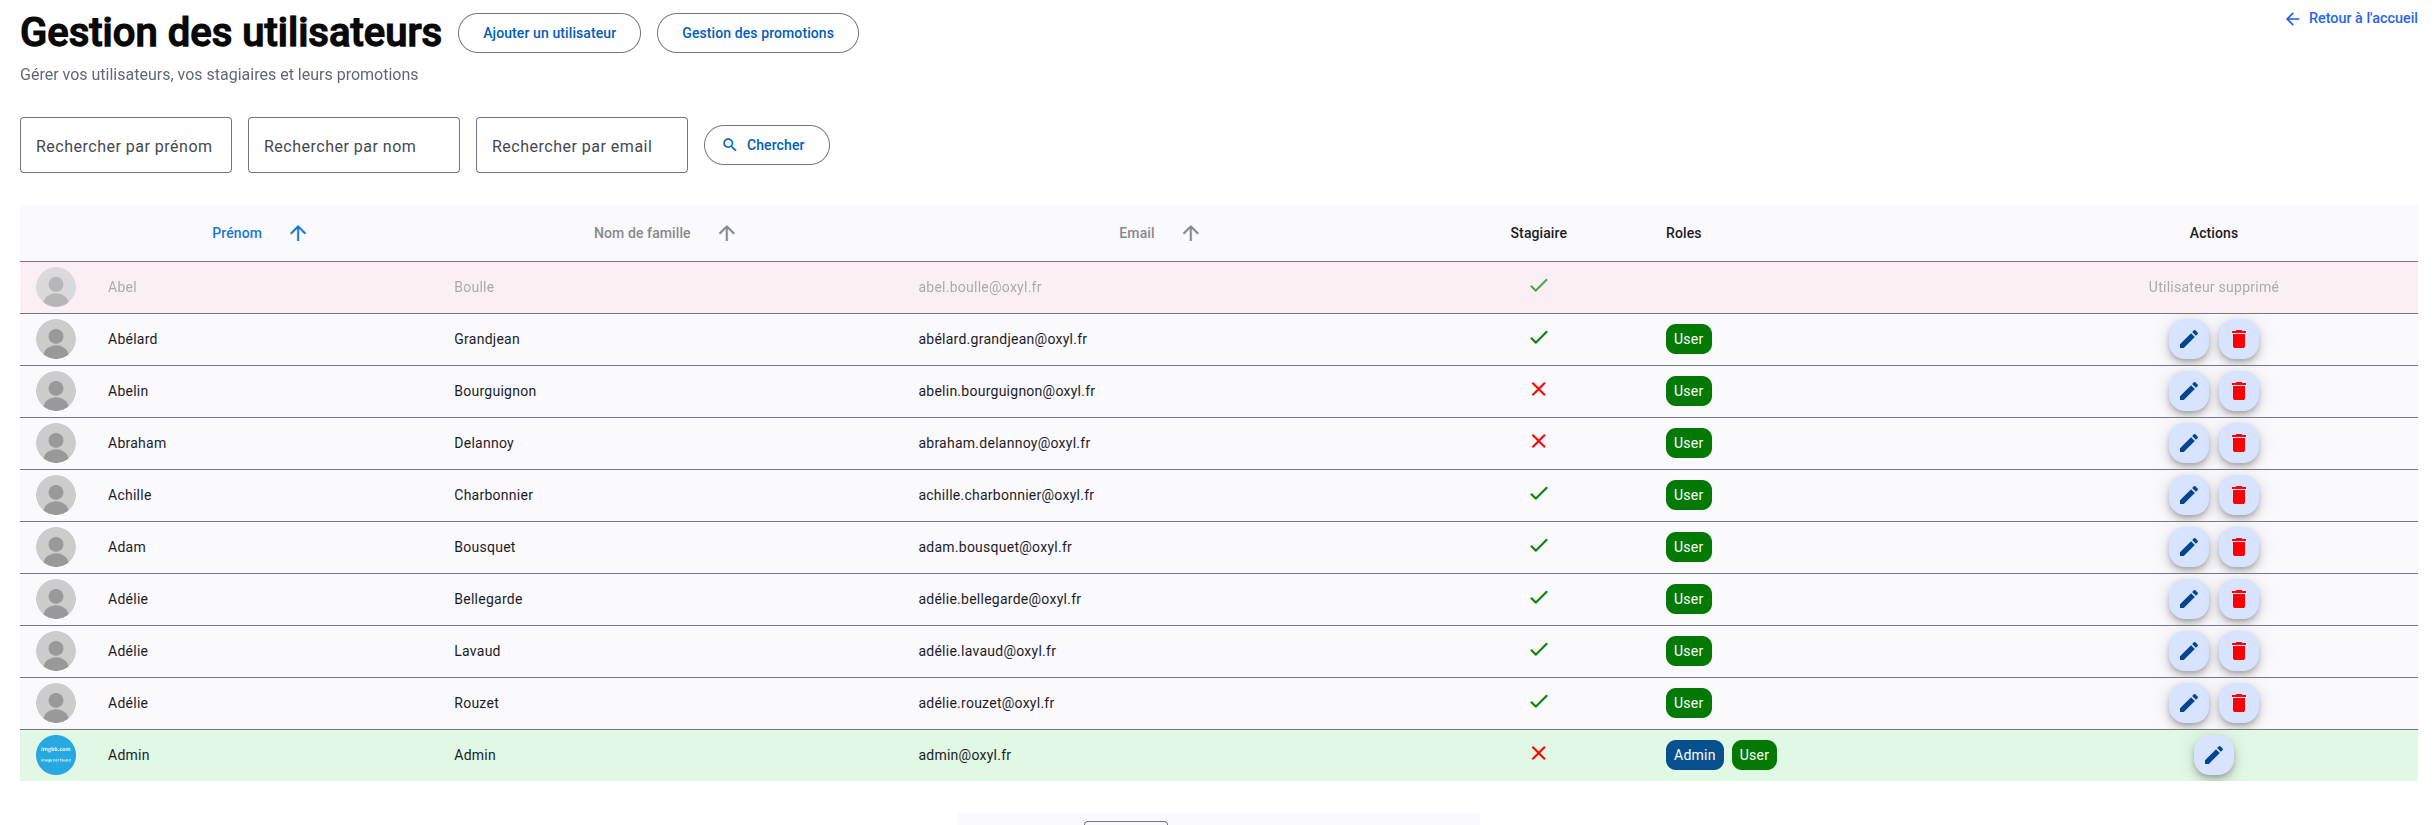
\includegraphics[width=0.92\textwidth]{figures/quiz_admin_users.png}
    \caption{Tableau de bord d'administration des utilisateurs : gestion des comptes, rattachement aux promotions et attribution des rôles applicatifs}
    \label{fig:ui_admin_users}
\end{figure}

\begin{figure}[htbp]
    \centering
    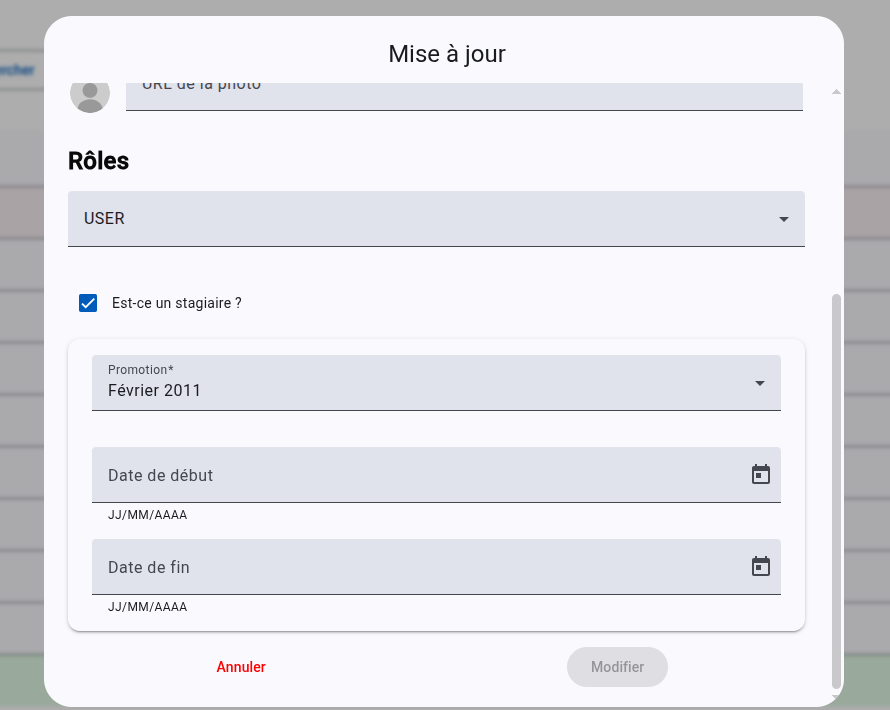
\includegraphics[width=0.68\textwidth]{figures/quiz_modal_edit_user.png}
    \caption{Boîte de dialogue modale de configuration d'un compte utilisateur (attribution des rôles, statut stagiaire, promotion et dates de stage)}
    \label{fig:ui_modal_edit_user}
\end{figure}

\subsubsection{Authentification JWT par cookies sécurisés et résolution CORS}
L'architecture applique un modèle sans état (\textit{stateless}) basé sur des jetons JSON Web Tokens (JWT) :
\begin{itemize}
    \item Pour immuniser le client contre les vulnérabilités de type \textit{Cross-Site Scripting} (XSS), le jeton JWT n'est pas stocké dans le \code{localStorage} du navigateur, mais encapsulé dans un cookie HTTP sécurisé (\code{HttpOnly}, \code{SameSite=Lax}) émis par la fabrique \code{AuthCookieFactory} ;
    \item La séparation physique en phase de développement et de déploiement entre le serveur front-end Angular (port $4200$) et l'API backend Spring (port $8080$) a nécessité une configuration rigoureuse du mécanisme de partage de ressources entre origines multiples (\textit{Cross-Origin Resource Sharing} - CORS).
\end{itemize}

Comme détaillé dans la classe \code{SecurityConfig}, l'instruction \code{configuration.setAllowCredentials(true)} a été combinée avec un filtrage explicite des motifs d'origine autorisés (\code{setAllowedOriginPatterns}) et l'autorisation des requêtes préliminaires d'évaluation (\textit{preflight} \code{OPTIONS}), garantissant ainsi l'acheminement transparent et inviolable des cookies d'authentification sur l'ensemble des endpoints REST.

\subsection{Conception de l'interface utilisateur et expérience apprenant (Angular)}
\label{subsec:conception_front_angular}

L'interface utilisateur a été conçue sous le framework Angular, en accordant une attention rigoureuse à l'ergonomie, à la clarté visuelle et à la rapidité de prise en main.

\subsubsection{Design System et architecture CSS}
J'ai pris en charge la conception de la feuille de style globale, du design system et de la mise en page générale de l'application. L'objectif était de rompre avec l'aspect utilitaire brut souvent associé aux outils internes d'entreprise, pour proposer une interface moderne et valorisante :
\begin{itemize}
    \item Définition d'une palette chromatique harmonieuse à base de variables CSS (couleurs sémantiques, contrastes validés selon les critères d'accessibilité WCAG) ;
    \item Mise en page responsive modulaire s'adaptant aussi bien aux postes de travail des développeurs qu'aux terminaux portables ;
    \item Conception de composants graphiques atomiques : cartes de lancement de quiz interactives (\texttt{card-quiz}), affichage de l'arborescence des chapitres avec indicateurs d'état et badges statistiques (\texttt{chapter-tree-node}), et boîte de dialogue modale de confirmation.
\end{itemize}

\subsubsection{Parcours utilisateur et navigation interactive}
Le front-end s'organise autour de parcours fluides pilotés par les services Angular et RxJS :
\begin{itemize}
    \item \textbf{Le tableau de bord stagiaire et diagnostic des compétences :} synthèse visuelle présentant la progression globale, l'accès rapide aux séries d'entraînement par module (Figure~\ref{fig:ui_stats_competence}) et la liste des derniers examens blancs passés ;
    \item \textbf{Le module de suivi des séries en cours :} interface permettant de reprendre à tout moment un questionnaire entamé avec filtrage par date et par taux de réussite (Figure~\ref{fig:ui_series_en_cours}) ;
    \item \textbf{Le portail d'administration :} interface réservée aux tuteurs permettant la gestion des promotions, la création des comptes stagiaires et la consultation directe des métriques individuelles.
\end{itemize}

\begin{figure}[htbp]
    \centering
    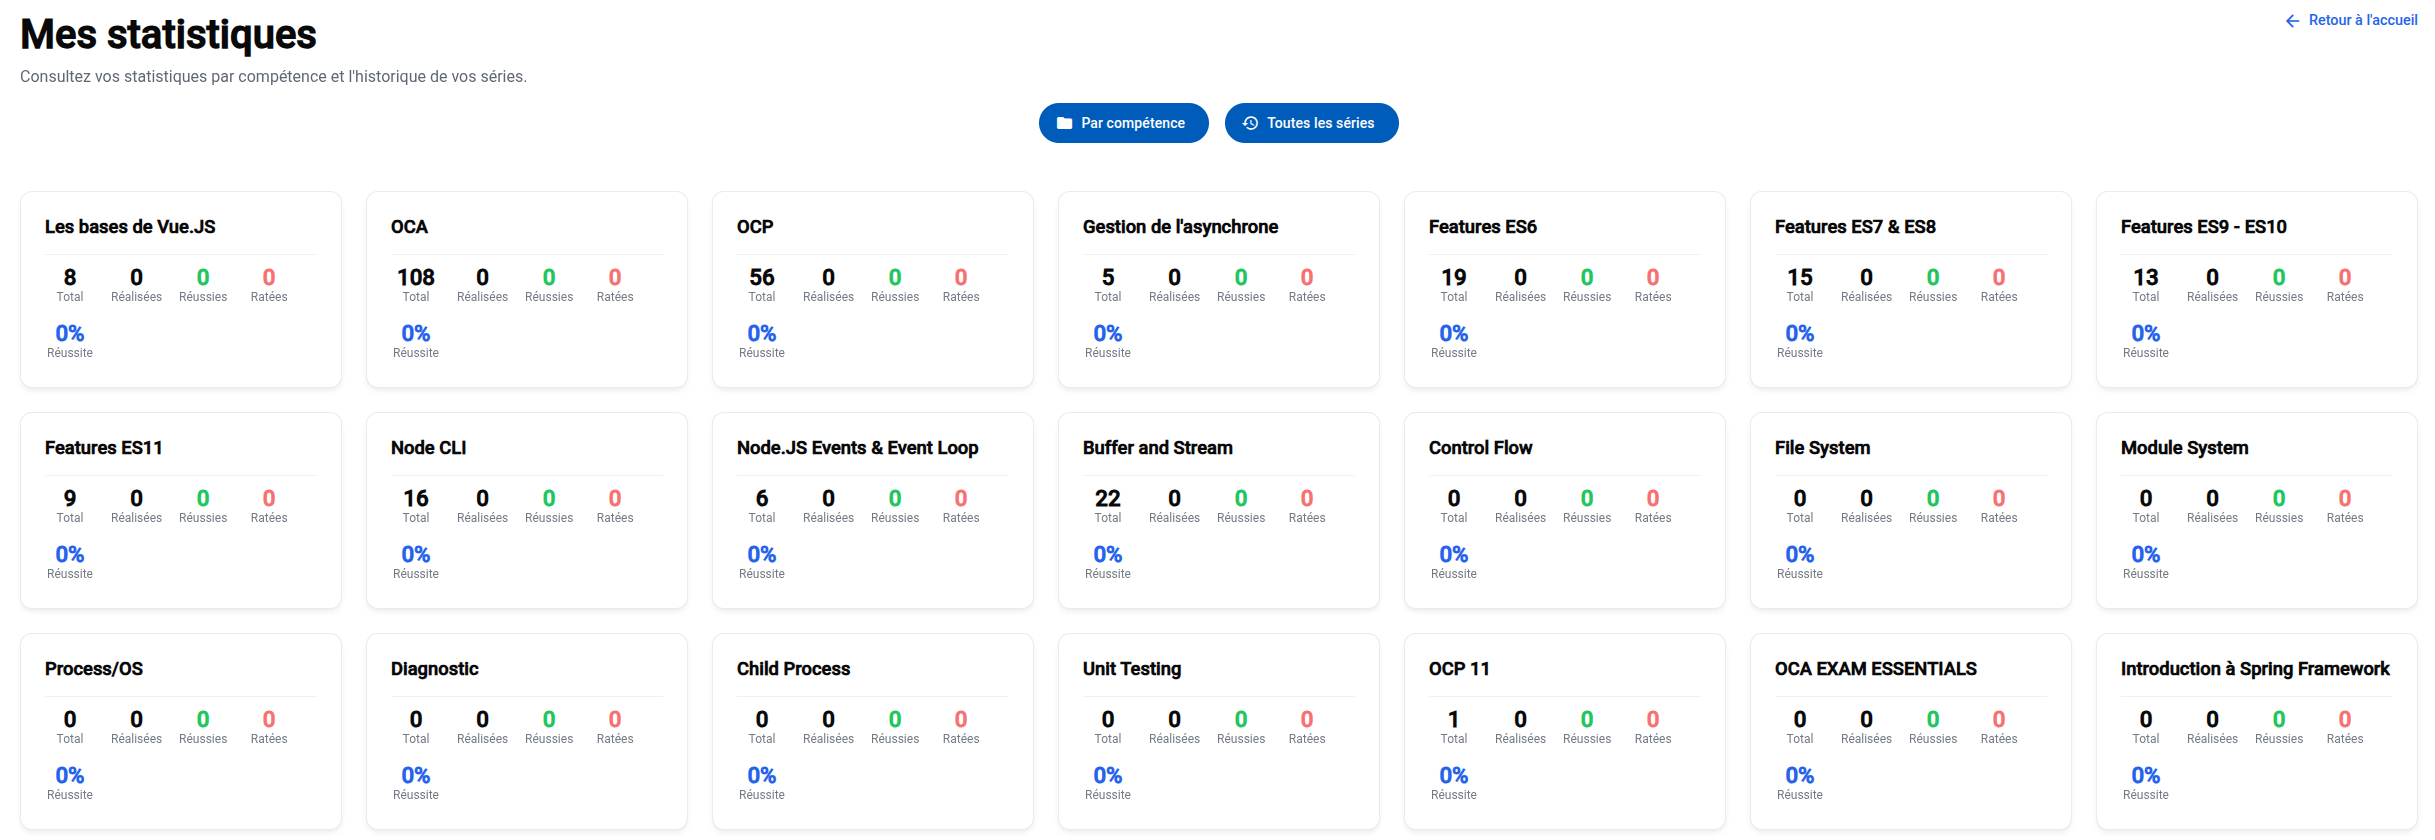
\includegraphics[width=0.92\textwidth]{figures/quiz_stats_par_competence.png}
    \caption{Tableau de bord analytique des compétences : suivi quantitatif de la progression (total, questions réussies/ratées et taux de succès)}
    \label{fig:ui_stats_competence}
\end{figure}

\begin{figure}[htbp]
    \centering
    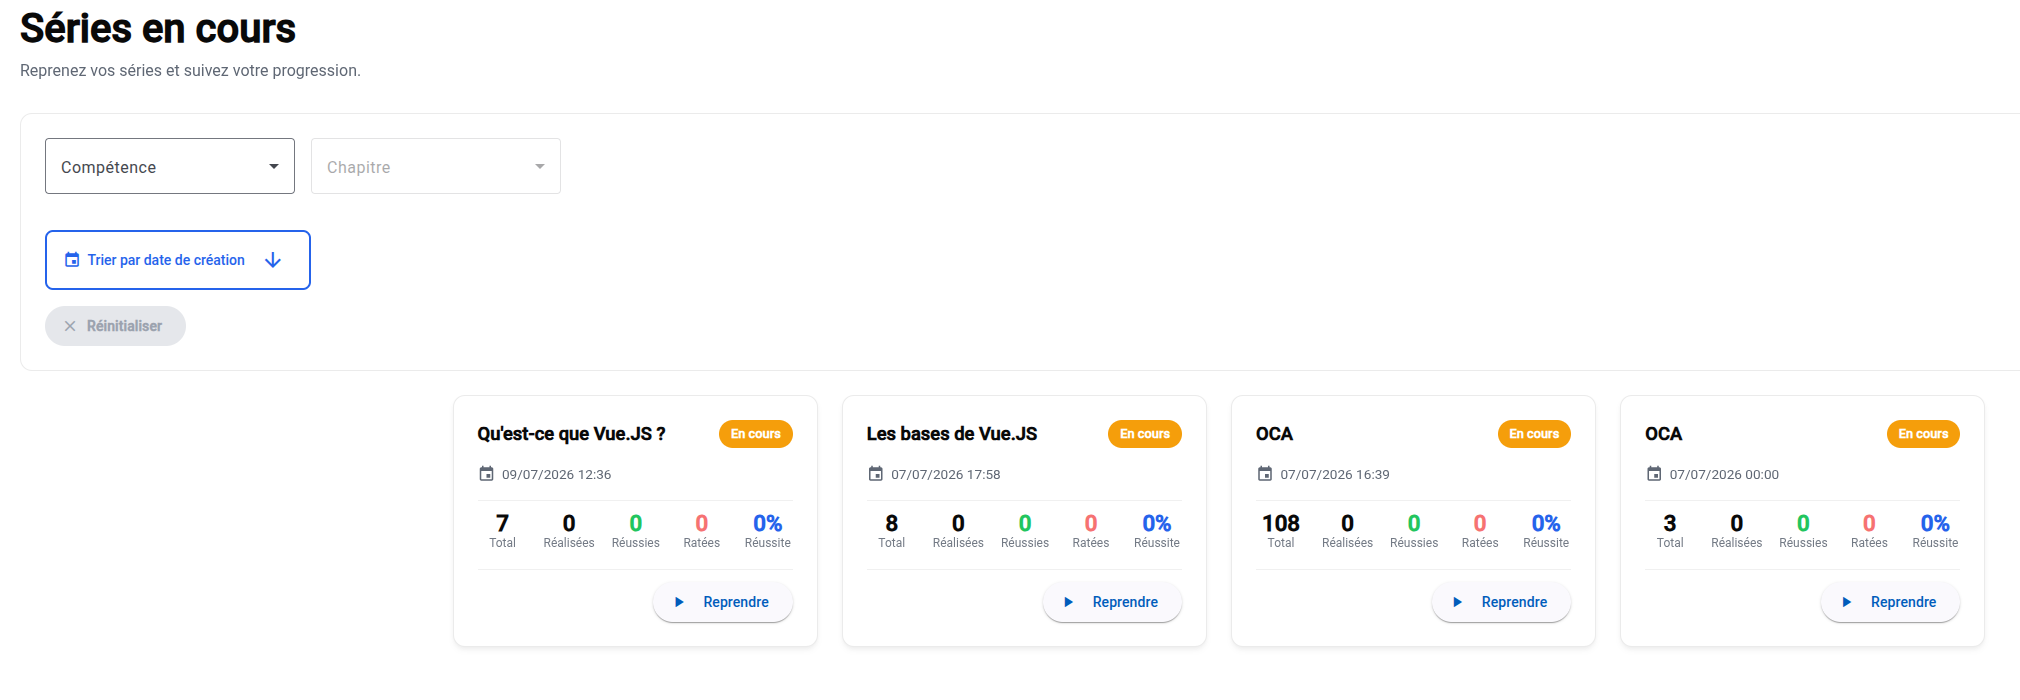
\includegraphics[width=0.92\textwidth]{figures/quiz_series_en_cours.png}
    \caption{Interface de suivi et de reprise des séries en cours : filtres multicritères et visualisation synthétique par carte}
    \label{fig:ui_series_en_cours}
\end{figure}

\subsection{Dynamique d'ingénierie collaborative, gestion des risques et retours d'expérience}
\label{subsec:dynamique_collaborative_rex}

Au-delà des aspects purement techniques de développement, la réalisation de \textit{NewroFactory} a constitué une expérience humaine et organisationnelle fondatrice sur la gestion de projet logiciel en équipe.

\subsubsection{Du développement individuel à l'intégration collective à 4}
Le calendrier du projet s'est articulé en deux phases méthodologiques très contrastées :
\begin{enumerate}
    \item \textbf{Phase 1 (Les 8 premiers sprints -- 2,5 mois) :} chaque stagiaire a développé individuellement son propre backend \textit{from scratch}, franchissant par l'épreuve les paliers successifs de l'ingénierie Java (du CLI natif et JDBC pur jusqu'à Spring Boot, Spring Security et Hibernate). Cette démarche a garanti l'alignement individuel de chacun sur les fondamentaux d'architecture ;
    \item \textbf{Phase 2 (Sprint collaboratif final) :} nous avons sélectionné l'un des backends développés parmi les quatre comme socle commun. L'ensemble des quatre stagiaires a ensuite été réuni pour travailler simultanément sur le développement du front-end Angular et l'ajustement des API backend.
\end{enumerate}

\subsubsection{Difficultés rencontrées et arbitrages méthodologiques}
Le passage brutal du travail en solitaire au développement simultané à quatre sur une base de code partagée a mis en lumière des défis d'ingénierie majeurs :
\begin{itemize}
    \item \textbf{Gestion des flux Git et conflits de fusion :} n'ayant jamais été confrontés à une collaboration synchrone aussi intensive, nous avons initialement fait face à des régressions et à des superpositions de code dues à un manque de régularité dans la synchronisation locale (\texttt{git pull}) avant d'entamer de nouvelles modifications. Pour résoudre ces frictions, nous avons dû formaliser une discipline rigoureuse de gestion des branches et veiller à une synchronisation quotidienne systématique ;
    \item \textbf{Découpage et respect des périmètres de tickets :} nous avons appris par l'expérience l'importance cruciale de définir des tickets de travail strictement atomiques et parfaitement délimités. Lorsque le périmètre d'un ticket débordait sur les modules adjacents, le risque de collision entre développeurs augmentait de manière critique ;
    \item \textbf{Synchronisation des schémas de base de données :} chaque membre de l'équipe travaillant sur une instance MySQL locale, toute évolution structurelle du modèle de données (ajout de colonnes, modifications de contraintes) devait être répercutée manuellement par des scripts SQL partagés, soulignant l'importance future d'outils de migration automatisés (tels que Flyway ou Liquibase) ;
    \item \textbf{Déploiement Cloud :} la plateforme a été déployée sur l'infrastructure Cloud d'Amazon Web Services, en exploitant une instance virtuelle \textbf{AWS EC2} pour l'exécution des conteneurs applicatifs et un stockage \textbf{AWS S3} pour les ressources et sauvegardes.
\end{itemize}

Cette première réalisation grandeur nature a ancré des réflexes d'ingénierie essentiels : rigueur du découpage fonctionnel, conception d'architectures résilientes et standardisation des livrables. Elle a établi le socle indispensable pour aborder le second défi d'envergure du stage : la conception d'une usine logicielle agentique industrialisée et agnostique.

\section{Choix techniques comme choix de maturité : Justification de l'architecture (Spring Core/Angular) pour une maîtrise approfondie des fondamentaux}
\label{sec:choix_techniques_quiz}
Les choix d'architecture technologique retenus pour la plateforme \textit{NewroFactory} procèdent d'un arbitrage réfléchi entre impératifs de formation, rigueur d'ingénierie et maîtrise pragmatique des délais de livraison. Loin d'être de simples sélections d'outils, ces choix constituent un véritable parti pris méthodologique visant la maîtrise des fondamentaux du développement logiciel moderne.

\subsection{Démystification des couches applicatives : Le choix de Spring Core et de la configuration explicite}
\label{subsec:choix_spring_core}

Alors que l'écosystème moderne privilégie l'utilisation immédiate de Spring Boot pour sa capacité à masquer la complexité derrière des starters auto-configurés, nous avons délibérément fait le choix d'édifier le backend sur le socle \textbf{Spring Core} et les bibliothèques Spring sous-jacentes de manière explicite.

Ce choix s'explique par la volonté de comprendre en profondeur la mécanique interne et l'articulation des couches composant une application web d'entreprise n-tiers. En renonçant à la « magie » des auto-configurations automatiques :
\begin{itemize}
    \item \textbf{Maîtrise du conteneur IoC et injection de dépendances :} nous avons configuré explicitement le contexte d'application, la déclaration et le cycle de vie des Beans métier, forçant une compréhension fine du principe d'Inversion de Contrôle (\textit{Inversion of Control} - IoC) et d'injection de dépendances ;
    \item \textbf{Configuration explicite des filtres et servlets :} la mise en œuvre manuelle de la chaîne de filtres de sécurité (\code{SecurityFilterChain}), du découplage des aspects de journalisation (\code{LoggingAspect}) et de la gestion des erreurs HTTP a permis d'appréhender le fonctionnement exact du moteur Web de Spring (\code{DispatcherServlet}) sans subir d'abstractions opaques ;
    \item \textbf{Appropriation de l'architecture n-tiers :} l'explicitation du passage de données entre les contrôleurs REST, les services transactionnels et la persistance relationnelle a renforcé les réflexes de découplage et d'isolation des responsabilités (\textit{Single Responsibility Principle}).
\end{itemize}

Ce parti pris d'ingénierie procède d'une conviction pédagogique forte chez Oxyl : maîtriser les bases fondamentales et les concepts sous-jacents (spécifications JEE, Servlet API, conteneur IoC, cycle de vie JVM) permet à un ingénieur d'appréhender sans effort l'ensemble des frameworks du marché plutôt que d'être captif d'une seule technologie. Une fois la mécanique de JEE et de Spring Core intimement assimilée, la prise en main d'architectures plus récentes comme \textbf{Spring Boot} ou d'alternatives \textit{cloud-native} telles que \textbf{Quarkus} ou \textbf{Micronaut} devient fluide et immédiate, l'ingénieur comprenant exactement les mécanismes d'optimisation (tels que la compilation native GraalVM ou l'injection au build-time) masqués par ces outils.

\subsection{Adoption d'Angular : Rigueur structurelle et opportunité de montée en compétences}
\label{subsec:choix_angular}

Côté frontend, le choix s'est porté sur le framework \textbf{Angular}. Ce choix répond à un double objectif technique et d'apprentissage :
\begin{itemize}
    \item \textbf{Rigueur architecturale et typage strict :} Angular impose une structure orientée composants, services et injection de dépendances particulièrement rigoureuse, véhiculée par le langage TypeScript. Ce typage strict à la compilation prémunit l'application contre toute une classe d'erreurs d'exécution et aligne la conception client sur les exigences de qualité du backend Java ;
    \item \textbf{Montée en compétences sur un framework d'entreprise :} par rapport à d'autres bibliothèques UI plus répandues dans le cadre académique (telles que React ou Vue.js), Angular est un framework complet mais plus exigeant. Ce projet représentait une opportunité privilégiée d'expérimenter et d'explorer une technologie robuste et largement éprouvée au sein des grands comptes industriels et des ESN.
\end{itemize}

\subsection{Monolithe modulaire vs Microservices : Pragmatisme et focalisation sur le prototype}
\label{subsec:choix_monolithe}

Sur le plan de l'architecture globale, nous avons opté pour un \textbf{monolithe modulaire} rigoureusement découpé en paquets métier. Ce choix résulte d'une décision d'ingénierie pragmatique dictée par deux facteurs majeurs :
\begin{itemize}
    \item \textbf{Respect du calendrier et gestion du temps :} le temps imparti pour cette phase de réalisation interdisait la sur-ingénierie liée aux architectures distribuées en microservices (gestion du réseau, découplage des bases de données par service, passerelles d'API et orchestration complexe) ;
    \item \textbf{Focus sur le livrable fonctionnel (POC) :} l'objectif prioritaire était de concevoir et présenter une preuve de concept (\textit{Proof of Concept} - POC) fonctionnelle, robuste, testable et de haute qualité dans les délais impartis, plutôt qu'un système sur-dimensionné. La structure monolithique modulaire garantit ainsi une cohérence transactionnelle immédiate tout en réservant la possibilité d'un découplage futur si le volume d'utilisateurs l'exigeait.
\end{itemize}

\subsection{Écosystème outillé et composants clés du socle technique}
\label{subsec:outils_socle_technique}

Pour compléter ce socle d'ingénierie, plusieurs outils et bibliothèques fondamentaux ont été intégrés et articulés :
\begin{itemize}
    \item \textbf{Apache Maven :} employé comme moteur de build standardisé et gestionnaire d'outils, assurant une gestion transparente des dépendances, la répétabilité des builds et le packaging en archive exécutable ;
    \item \textbf{Hibernate et JPA (\textit{Java Persistence API}) :} assurent l'abstraction relationnelle et la correspondance objet-relationnel (ORM), permettant la manipulation fluide des entités métier (\code{ChapterEntity}, \code{QuestionEntity}) et l'exécution optimisée des requêtes ;
    \item \textbf{Jakarta Validation :} utilisé pour garantir la validation déclarative et systématique des DTOs en entrée d'API (\code{@NotNull}, \code{@Size}, validateurs personnalisés), assurant l'étanchéité des données saisies ;
    \item \textbf{JJWT (Java JWT) :} exploité pour la création et la vérification cryptographique des jetons d'authentification JSON Web Tokens, sécurisant les échanges de session de manière stateless via des cookies HTTP sécurisés.
\end{itemize}


\cleardoublepage

\chapter{La standardisation du capital technique (Volet 2 - L'usine IA)}
\label{chap:usine_ia}

\section{État de l'art : L'industrialisation du cycle de vie logiciel (SDLC) et les agents IA (SWE-bench)}
\label{sec:etat_de_l_art}

L'intégration des modèles de langage de grande taille (\textit{Large Language Models} - LLMs) au sein du cycle de vie du développement logiciel (\textit{Software Development Life Cycle} - SDLC) représente une transition majeure dans la manière d'analyser, de concevoir et d'entretenir les systèmes d'information. Longtemps cantonnée à de l'assistance contextuelle ponctuelle, l'automatisation s'oriente désormais vers des architectures agentiques capables d'exécuter de manière autonome des sous-ensembles complexes du SDLC.

\subsection{L'évolution du SDLC et la primauté de la génération de code}
\label{subsec:evolution_sdlc}

Parmi l'ensemble des phases constitutives du SDLC --- analyse des besoins, modélisation architecturale, développement, revue de code, tests d'intégration et déploiement --- l'étape de \textbf{génération et de modification de code} constitue le verrou le plus stratégique et le plus consommateur de ressources.

Historiquement, l'évaluation des capacités des LLMs s'appuyait sur des jeux de données synthétiques tels que HumanEval~\cite{chen2021codex} ou MBPP, mesurant la génération d'une fonction isolée à partir d'une spécification courte. Bien que pertinents pour valider la compréhension algorithmique de base, ces indicateurs s'avèrent insuffisants pour représenter l'ingénierie logicielle industrielle, caractérisée par des dépôts volumineux, des dépendances inter-fichiers et la nécessité de respecter des patrons d'architecture préexistants.

L'industrialisation moderne du SDLC requiert ainsi des modèles non seulement capables de rédiger de nouvelles implémentations, mais surtout de naviguer au sein de bases de code existantes, de diagnostiquer des régressions, et de proposer des diffs directement intégrables au workflow d'intégration continue (CI/CD).

Dans la vision d'Oxyl, le point d'entrée universel de l'usine logicielle est le \textbf{ticket d'ingénierie} (issu indifféremment de GitLab Issues, GitHub Issues ou Jira). Cette approche unifiée permet d'adresser sans restriction l'intégralité du cycle de vie logiciel :
\begin{itemize}
    \item \textbf{La maintenance corrective (\textit{bug fixing}) :} reproduction automatisée de l'anomalie, isolation de la régression et génération du patch de correction ;
    \item \textbf{Le développement de fonctionnalités (\textit{feature delivery}) :} implémentation de nouveaux services ou composants à partir de spécifications fonctionnelles formalisées ;
    \item \textbf{La maintenance préventive et le nettoyage technique (\textit{refactoring / tech debt}) :} modernisation de dépendances, migration de syntaxe, typage strict et élimination de code mort.
\end{itemize}

\subsection{Évaluation agentique par SWE-bench et assistants en ligne de commande}
\label{subsec:swebench_cli}

Pour répondre aux limites des métriques de génération synthétiques, le benchmark \textbf{SWE-bench}~\cite{jimenez2023swebench} s'est imposé comme l'étalon-or scientifique pour l'évaluation des agents autonomes de génie logiciel. Basé sur l'extraction de tickets réels issues de projets open-source Python d'envergure, SWE-bench confronte l'agent à une description de problème et à l'état complet du dépôt Git. La réussite est conditionnée par la capacité de l'agent à générer un patch validant l'ensemble de la suite de tests unitaires du projet sans introduire de régression.

Dans une perspective d'intégration opérationnelle au court terme, le choix des interfaces d'exécution s'oriente vers des outils joignables par \textbf{ligne de commande (CLI)}, notamment :
\begin{itemize}
    \item \textbf{Google Antigravity SDK :} permettant l'orchestration dynamique d'agents et de sous-agents autonomes spécialisés pour le suivi de tâches complexes ;
    \item \textbf{OpenAI Codex / CLI :} fournissant des capacités d'édition directe et de modification raisonnée de fichiers source ;
    \item \textbf{Claude Code CLI :} offrant des capacités avancées de raisonnement à fenêtre de contexte étendue et d'exécution d'instructions shell interactives.
\end{itemize}

L'évaluation de ces outils à l'aide de SWE-bench permet de qualifier rigoureusement leur niveau d'autonomie et leur résilience face à la complexité des tâches d'ingénierie.

\subsection{Analyse comparative des solutions agentiques du marché}
\label{subsec:comparatif_marche}

Face à la multiplication des solutions commerciales et open-source d'assistance agentique (telles que Devin, GitHub Copilot Workspace, Cursor ou SWE-agent~\cite{yang2024sweagent}), une analyse comparative s'impose pour positionner la stratégie retenue au sein d'Oxyl.

Le Tableau~\ref{tab:comparatif_agents} synthétise la comparaison entre l'approche d'usine logicielle agnostique développée et les solutions majeures du marché selon quatre critères fondamentaux.

\begin{table}[htbp]
\centering
\caption{Analyse comparative des solutions agentiques du marché vs l'Usine IA Oxyl}
\label{tab:comparatif_agents}
\footnotesize
\begin{tabularx}{\textwidth}{|l|X|X|X|X|}
\hline
\textbf{Solution} & \textbf{Intégration CLI / CI-CD} & \textbf{Agnosticisme LLM (Anti lock-in)} & \textbf{Scope d'édition code} & \textbf{Extensibilité des workflows} \\ \hline
\textbf{GitHub Copilot} & Faible (IDE/Web) & Propriétaire (OpenAI) & Fichier / In-line & Limitée (Extensions) \\ \hline
\textbf{Devin / SaaS proprietary} & Web / Clôturé & Propriétaire / Intégré & Projet complet & Configurable (SaaS) \\ \hline
\textbf{Cursor / Claude Code} & CLI / IDE local & Multi-modèles restreint & Projet complet & Scriptable \\ \hline
\textbf{Usine IA Oxyl (Proposée)} & \textbf{Native CLI \& CI-CD} & \textbf{Agnostique (Google/OpenAI/Claude)} & \textbf{Multi-fichiers complet} & \textbf{Totale (Patrons de conception \& SDK)} \\ \hline
\end{tabularx}
\end{table}

Cette analyse met en évidence que l'usine logicielle Oxyl privilégie l'indépendance technologique et la personnalisation fine des flux agentiques, combinant la souplesse d'exécution CLI à un contrôle total sur l'infrastructure de développement.

\section{Théorie de l'abstraction : Étude des patrons de conception pour s'affranchir du lock-in}
\label{sec:theorie_abstraction}

L'intégration d'assistants et d'agents d'intelligence artificielle au sein d'une usine logicielle industrielle confronte l'architecture à un risque majeur d'enfermement technologique (\textit{vendor lock-in}). Les fournisseurs de modèles de langage (LLMs) et d'outils agentiques --- tels qu'Anthropic (Claude Code), Google (Antigravity SDK / Gemini) ou OpenAI (Codex / GPT) --- imposent des interfaces de programmation, des formats d'outillage (\textit{tool-calling}), des protocoles d'authentification et des modes d'exécution profondément disparates.

Pour garantir la pérennité de l'usine logicielle, son indépendance stratégique et la substituabilité immédiate d'un modèle par un autre sans réécriture du cœur applicatif, nous avons mené une étude approfondie des patrons de conception logicielle (\textit{design patterns}) dédiés à l'abstraction.

\subsection{Dilemme d'ingénierie et arbitrage des patrons de conception}
\label{subsec:arbitrage_patterns}

La conception du socle d'abstraction agentique a nécessité la confrontation de plusieurs patrons classiques du \textit{Gang of Four} (GoF) :

\begin{itemize}
    \item \textbf{L'Adapter (Adaptateur) :} Ce patron a été retenu comme le pivot conceptuel de l'architecture. La relation entre le moteur d'orchestration de l'usine et les différents moteurs d'IA est fondamentalement une relation de \textbf{traduction} : il s'agit de convertir des requêtes canoniques d'ingénierie (prompts, outils autorisés, contextes d'exécution) vers les syntaxes d'invocation spécifiques à chaque fournisseur (flags CLI, schémas JSON d'outils, flux d'entrée standard) et d'en normaliser les retours.
    \item \textbf{La Strategy (Stratégie) :} Le patron Strategy a été abondamment étudié et s'hybride naturellement avec notre implémentation de l'Adapter. Le moteur applicatif interagit avec une interface générique stable (\code{LLMProvider} / \code{AgentRunner}) définissant les signatures des méthodes d'invocation. Les classes d'adaptation concrètes implémentent ces méthodes selon les spécificités de chaque modèle. Le choix du moteur à solliciter étant résolu dynamiquement à l'exécution selon le profil de la tâche, l'interchangeabilité de l'algorithme sous-jacent s'apparente à une Strategy.
    \item \textbf{Le Bridge (Pont) :} Le patron Bridge permet de découpler une hiérarchie d'abstractions (les types d'activités logicielles : analyse de ticket, génération de code, audit de sécurité) de multiples hiérarchies d'implémentations (les protocoles d'exécution CLI, API REST, WebSocket). Bien que séduisant, son adoption complète a été écartée au profit d'une interface d'adaptation plus directe afin d'éviter une sur-ingénierie prématurée.
    \item \textbf{Abstract Factory vs Singleton pour l'instanciation :} L'instanciation de l'adaptateur a fait l'objet d'un arbitrage spécifique. Si une \textit{Factory} (fabrique) a été envisagée pour instancier dynamiquement l'adaptateur requis, nous avons opté pour la conservation d'une instance unique (\textbf{Singleton}) en mémoire durant toute la durée de vie d'un conteneur worker. L'accès à cet adaptateur s'effectue via un résolveur dédié (\code{getLLMProvider()}), combinant ainsi la flexibilité d'une fabrique à la cohérence d'un point d'accès persistant en mémoire.
\end{itemize}

\subsection{Modélisation de la couche d'abstraction des moteurs d'IA}
\label{subsec:modelisation_abstraction_llm}

L'architecture d'abstraction projetée pour les moteurs LLM s'articule autour d'une interface canonique commune, d'un résolveur dynamique et d'adaptateurs spécialisés par fournisseur. Cette démarche reproduit fidèlement les principes d'abstraction déjà validés sur les composants de gestion de versions et de tickets.

La Figure~\ref{fig:diagramme_uml_adapter_llm} schématise cette organisation structurelle.

\begin{figure}[htbp]
\centering
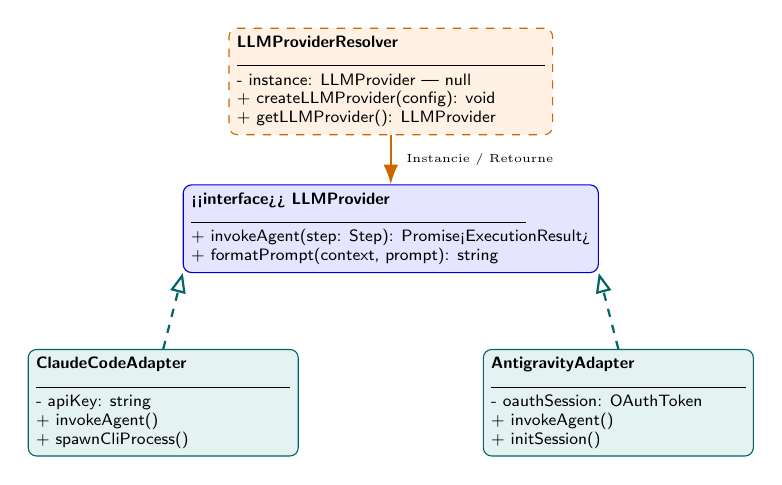
\begin{tikzpicture}[
    scale=0.85,
    transform shape,
    font=\sffamily\scriptsize,
    interface/.style={draw=blue!80!black, fill=blue!10, rounded corners=3pt, minimum width=5.2cm, minimum height=1.3cm, align=left},
    adapter/.style={draw=teal!80!black, fill=teal!10, rounded corners=3pt, minimum width=4.0cm, minimum height=1.3cm, align=left},
    resolver/.style={draw=orange!80!black, fill=orange!10, dashed, rounded corners=3pt, minimum width=4.8cm, minimum height=1.2cm, align=left},
    arrow/.style={-{Latex[length=2.5mm]}, thick, draw=orange!80!black},
    impl/.style={-{Triangle[open, length=2.5mm]}, dashed, thick, draw=teal!80!black}
]
    % Nodes
    \node[interface] (provider) at (0, 0) {
        \textbf{<<interface>> LLMProvider}\\
        \rule{5.0cm}{0.4pt}\\
        + invokeAgent(step: Step): Promise<ExecutionResult>\\
        + formatPrompt(context, prompt): string
    };
    
    \node[adapter] (claude) at (-3.4, -2.6) {
        \textbf{ClaudeCodeAdapter}\\
        \rule{3.8cm}{0.4pt}\\
        - apiKey: string\\
        + invokeAgent()\\
        + spawnCliProcess()
    };
    
    \node[adapter] (antigravity) at (3.4, -2.6) {
        \textbf{AntigravityAdapter}\\
        \rule{3.8cm}{0.4pt}\\
        - oauthSession: OAuthToken\\
        + invokeAgent()\\
        + initSession()
    };
    
    \node[resolver] (resolver) at (0, 2.2) {
        \textbf{LLMProviderResolver}\\
        \rule{4.6cm}{0.4pt}\\
        - instance: LLMProvider | null\\
        + createLLMProvider(config): void\\
        + getLLMProvider(): LLMProvider
    };

    % Links
    \draw[impl] (claude.north) -- (provider.south west);
    \draw[impl] (antigravity.north) -- (provider.south east);
    \draw[arrow] (resolver.south) -- node[right=3pt, font=\tiny] {Instancie / Retourne} (provider.north);
\end{tikzpicture}
\caption{Diagramme conceptuel du patron Adapter appliqué au découplage des moteurs LLM}
\label{fig:diagramme_uml_adapter_llm}
\end{figure}

Le contrat d'interface \code{LLMProvider} définit une frontière étanche : le code métier de l'usine logicielle (gestion des étapes du workflow, validation mécanique, persistance des états) n'a aucune dépendance directe envers les SDKs ou binaires propriétaires.

\subsection{Défis d'abstraction et contraintes d'exécution conteneurisée}
\label{subsec:defis_abstraction_llm}

L'unification des moteurs d'intelligence artificielle au sein d'environnements d'exécution automatisés (conteneurs Docker isolés et sans interface graphique) met en exergue des disparités techniques majeures que l'adaptateur doit normaliser :

\begin{enumerate}
    \item \textbf{Hétérogénéité des protocoles d'accès et d'authentification :}
    \begin{itemize}
        \item \textbf{Claude Code CLI :} Fonctionne nativement en ligne de commande autonome. Son exécution au sein du conteneur repose sur l'injection de variables d'environnement (\code{ANTHROPIC_API_KEY}), l'invocation d'un sous-processus sans état (\code{spawnSync}) et la transmission du prompt par le flux d'entrée standard (\code{stdin}) ;
        \item \textbf{Google Antigravity SDK :} Conçu originellement pour opérer comme une extension intégrée à un environnement de développement interactif (IDE), son intégration dans un conteneur headless autonome nécessite une couche d'émulation de session et la gestion d'un jeton d'authentification OAuth spécifique.
    \end{itemize}

    \item \textbf{Gestion granulaire de l'outillage (\textit{Tool Gating}) :}
    Tous les modèles ne disposent pas des mêmes conventions de déclaration d'outils. La couche d'abstraction normalise l'allocation des capacités selon la sensibilité de l'étape :
    \begin{itemize}
        \item Les étapes marquées \code{read_only} (audits, revues de code) ne transmettent aux adaptateurs que les outils d'exploration et de consultation (\code{Read}, \code{Glob}, \code{Grep}) et de rapport (\code{Write}), tout en désactivant strictement l'outil de modification de code source (\code{Edit}) ;
        \item Les étapes de développement ouvrent l'ensemble des capacités d'édition et d'exécution de commandes.
    \end{itemize}

    \item \textbf{Normalisation des retours et injection contextuelle de résilience :}
    En cas d'échec d'une étape (erreur de compilation ou régression de tests), l'adaptateur injecte de manière transparente un bloc structuré de remédiation (\textit{Retry Context}) en amont du prompt pour guider le modèle lors de la tentative suivante, tout en assurant l'assainissement automatique (\code{redactSecrets}) de toutes les sorties pour prévenir la fuite d'informations sensibles dans les journaux d'audit.
\end{enumerate}

Cette conception modulaire garantit ainsi une agnosticité totale : l'ajout d'un nouveau fournisseur (par exemple un modèle open-source hébergé localement via Ollama ou vLLM) se résume à l'écriture d'une nouvelle classe implémentant \code{LLMProvider} sans impacter le reste du pipeline d'ingénierie.

\section{Analyse des contraintes : Sécurité, gestion des coûts de tokens et reproductibilité des résultats}
\label{sec:analyse_contraintes}

L'exploitation industrielle d'agents autonomes au sein du cycle de développement logiciel ne saurait se résumer à des considérations algorithmiques. En environnement de production, le déploiement de ces systèmes fait face à des contraintes opérationnelles strictes : la dérive financière liée à la consommation incontrôlée de tokens, la saturation des fenêtres de contexte, la préservation des secrets applicatifs et le caractère non déterministe des modèles génératifs.

Cette section détaille les mécanismes de contrôle, de résilience et de gouvernance mécanique mis en place pour garantir la viabilité économique, technique et sécuritaire de l'usine logicielle.

\subsection{Maîtrise des coûts et des temps d'exécution : Le double verrou de réessai}
\label{subsec:gestion_couts_tokens}

L'un des risques majeurs inhérents aux systèmes agentiques réside dans le phénomène de « boucle de raisonnement infinie » (\textit{infinite reasoning loop}). Lorsqu'un modèle se heurte à une anomalie sans parvenir à la corriger, il tend à multiplier les essais infructueux, engendrant une consommation exponentielle de tokens et un temps d'occupation critique des conteneurs.

Pour juguler ce risque, notre moteur intègre une politique de plafonnement à deux niveaux (illustrée en Figure~\ref{fig:resilience_retry_verrou}) :
\begin{itemize}
    \item \textbf{Plafond local par étape (\code{max_retries}) :} Chaque étape élémentaire du workflow d'un worker (par exemple la génération de code, l'analyse d'architecture ou l'exécution de la suite de tests) est assortie d'un quota strict de tentatives. Si une étape échoue (erreur de compilation, échec de linting), le moteur évalue le nombre d'essais consommés (\code{getRetryCount(step.id)}). Tant que \code{retryCount < step.max_retries}, une nouvelle tentative ciblée est autorisée ; dans le cas contraire, le traitement de l'étape est interrompu.
    \item \textbf{Disjoncteur global par ticket (\code{Circuit Breaker}) :} Au-delà des limites par étape, un compteur d'essais cumulés (\code{globalAttempts}) est maintenu pour l'ensemble du cycle de vie du worker sur un ticket donné. Dès que ce compteur atteint le seuil critique \code{maxGlobalAttempts} (défini par les limites globales de l'usine), le disjoncteur se déclenche immédiatement (\textit{circuit breaker triggered}), interrompant définitivement le traitement afin d'éviter tout surcoût financier ou blocage de la file de tâches.
    \item \textbf{Routage conditionnel sur échec (\code{on_fail} et \code{max_on_fail}) :} Lorsqu'une défaillance survient, le moteur analyse et classifie l'erreur (\code{classifyFailure}). Si un gestionnaire de déviation est configuré (ex. \code{goto diagnostic_step}), le flux est redirigé vers une étape spécialisée, tout en plafonnant le nombre total de déviations via \code{max_on_fail} pour empêcher les cycles de redirection infinis.
\end{itemize}

\begin{figure}[htbp]
\centering
\begin{tikzpicture}[
    scale=0.86,
    transform shape,
    font=\sffamily\scriptsize,
    statebox/.style={draw=blue!80!black, fill=blue!6, rounded corners=3pt, align=center, inner sep=6pt, line width=0.7pt, minimum width=3.2cm},
    decision/.style={draw=orange!80!black, fill=orange!8, diamond, aspect=1.8, align=center, inner sep=2.5pt, line width=0.7pt, font=\sffamily\bfseries\tiny},
    errbox/.style={draw=red!70!black, fill=red!6, rounded corners=2pt, align=left, inner sep=4pt, font=\sffamily\tiny, text width=3.0cm},
    succbox/.style={draw=teal!80!black, fill=teal!8, rounded corners=2pt, align=center, inner sep=4pt, font=\sffamily\bfseries\tiny, text width=2.8cm},
    flowarrow/.style={-{Latex[length=2.5mm]}, thick, draw=blue!80!black}
]

    % Étape 1 : Exécution LLM
    \node[statebox] (exec) at (0, 3.8) {\textbf{Exécution de l'Étape}\\Invocation LLM (Claude CLI)};
    
    % Étape 2 : Évaluation résultat
    \node[decision] (eval) at (0, 1.8) {Succès de\\l'étape ?};

    % Branche Succès
    \node[statebox, fill=teal!6, draw=teal!80!black] (val) at (5.0, 1.8) {\textbf{Validation Mécanique}\\(\code{validateMechanical})};
    \node[succbox, below=0.2cm of val] (commit) {$\checkmark$ Commit de progrès (SHA)\\\code{manifest.json} mis à jour\\$\rightarrow$ Étape suivante};

    % Branche Échec & Disjoncteur
    \node[statebox, fill=red!4, draw=red!70!black] (classif) at (-5.0, 1.8) {\textbf{Classification de l'erreur}\\(\code{classifyFailure})};
    \node[errbox, below=0.2cm of classif] (errdetail) {
        $\bullet$ Type: \code{syntax_error / test_fail}\\
        $\bullet$ Erreur extraite \& tronquée\\
        $\bullet$ Incrément compteurs
    };

    \node[decision] (breaker) at (-5.0, -1.6) {Vérification\\Plafonds ?};

    \node[statebox, fill=purple!6, draw=purple!80!black] (retry) at (0, -1.6) {\textbf{Compression Contextuelle}\\(\code{buildRetryContext})};
    \node[succbox, fill=purple!8, draw=purple!70!black, below=0.2cm of retry] (retrydetail) {Injection minimale de l'erreur en tête de prompt\\$\rightarrow$ Ré-essai ciblé sans pollution contextuelle};

    \node[statebox, fill=red!10, draw=red!90!black] (halt) at (-5.0, -3.8) {\textbf{Arrêt Sécurisé \& Notification}\\Disjoncteur déclenché (Circuit Breaker)};

    % Flèches
    \draw[flowarrow] (exec) -- (eval);
    \draw[flowarrow, draw=teal!80!black] (eval) -- node[above, font=\sffamily\bfseries\tiny, text=teal!80!black] {OUI} (val);
    \draw[flowarrow, draw=teal!80!black] (val) -- (commit);

    \draw[flowarrow, draw=red!70!black] (eval) -- node[above, font=\sffamily\bfseries\tiny, text=red!70!black] {NON} (classif);
    \draw[flowarrow, draw=red!70!black] (classif) -- (errdetail);
    \draw[flowarrow, draw=red!70!black] (errdetail) -- (breaker);

    \draw[flowarrow, draw=teal!80!black] (breaker) -- node[above, font=\sffamily\bfseries\tiny, text=teal!80!black] {$\text{retries} < \text{Max}$} (retry);
    \draw[flowarrow, draw=purple!80!black] (retry) -- ++(3.2,0) |- (exec);

    \draw[flowarrow, draw=red!90!black] (breaker) -- node[right, font=\sffamily\bfseries\tiny, text=red!90!black] {Seuil atteint} (halt);

\end{tikzpicture}
\caption{Cycle de résilience et gouvernance mécanique : double verrou de réessai, disjoncteur et compression contextuelle par le Manifest}
\label{fig:resilience_retry_verrou}
\end{figure}

\subsection{Gestion du flux de sortie et compression contextuelle : Le rôle du Manifest}
\label{subsec:gestion_flux_manifest}

L'exécution des agents génère des volumes considérables de données textuelles (traces d'exécution, diffs de code, journaux de compilation). L'injection brute et intégrale de ces flux dans les invites d'entrée (\textit{prompts}) saturerait rapidement la fenêtre de contexte du modèle, provoquant une dégradation notable du raisonnement et un gonflement tarifaire.

Pour rationaliser ces flux de sortie, nous appliquons une stratégie de gestion asymétrique :
\begin{itemize}
    \item \textbf{Filtrage et affichage sélectif dans le terminal :} Les sorties brutes générées par les sous-processus ne sont pas intégralement imprimées dans la console standard. Le moteur de logs tronque les réponses volumineuses en conservant uniquement le début et la fin du message (\textit{head-and-tail truncation}), garantissant ainsi la lisibilité pour les développeurs tout en évitant la saturation des flux d'observabilité.
    \item \textbf{Persistance structurée dans le \textit{Manifest} :} Plutôt que de conserver l'historique complet des échanges en mémoire vive, les informations vitales d'état sont persistées au sein d'un document structuré machine-readable nommé \textbf{Manifest} (\code{manifest.json}). Ce fichier consigne l'identifiant de l'étape en cours, le numéro de tentative (\code{attemptNumber}), l'étape ayant échoué (\code{failedStep}) ainsi qu'un extrait synthétique de l'erreur (\code{errorSnippet}) et une recommandation d'orientation (\code{suggestion}).
    \item \textbf{Injection minimale de contexte de réessai (\textit{Retry Context}) :} Lors d'une reprise après incident, la fonction \code{buildRetryContext} n'extrait du Manifest que la charge utile essentielle liée à l'erreur précédente. Ce condensé contextuel est injecté en tête de prompt sous forme de directive ciblée (\textit{« Previous failure category: syntax\_error... »}), permettant au modèle de corriger son approche sans gaspiller de précieux tokens à relire des milliers de lignes de logs inutiles.
\end{itemize}

\subsection{Sécurité, étanchéité des conteneurs et assainissement des secrets}
\label{subsec:securite_secrets}

L'exécution autonome d'instructions shell et la manipulation de code source par des modèles tiers exigent un cadre de sécurité intransigeant. Chez Oxyl, la posture opérationnelle consiste à s'adapter rigoureusement aux politiques de sécurité et de conformité de chaque client :
\begin{itemize}
    \item \textbf{Adaptation aux politiques de gouvernance client :} pour les clients appliquant des règles d'étanchéité strictes (secteur bancaire, défense), l'usine est déployée en environnement fermé avec des modèles exécutés localement (\textit{on-premise}) sans aucun transit de données vers l'extérieur. Pour les clients autorisant les services d'inférence Cloud, les flux s'appuient sur des accords d'entreprise garantissant la non-rétention des données (\textit{zero-data retention}) ;
    \item \textbf{Isolation en conteneurs éphémères :} Chaque agent s'exécute au sein d'un conteneur Docker dédié, instancié à la volée avec des privilèges restreints et détruit à l'issue de la tâche. Cette conteneurisation garantit l'étanchéité totale du système hôte vis-à-vis des commandes exécutées par l'IA ;
    \item \textbf{Purification systématique des flux (\code{redactSecrets}) :} Les variables d'environnement des conteneurs hébergent des identifiants sensibles (clés d'API LLM, tokens Git). Une fonction d'assainissement intercepte et masque systématiquement ces secrets au sein des flux \code{stdout}, \code{stderr} et des messages d'erreur avant toute sauvegarde dans les rapports d'audit ou affichage dans les logs ;
    \item \textbf{Cloisonnement des permissions d'outils (\textit{Tool Gating}) :} Conformément au principe du moindre privilège, les étapes ne nécessitant pas de modification de code (revue, vérification) se voient interdire l'accès à l'outil d'écriture de code (\code{Edit}), restreignant ainsi la surface d'attaque.
\end{itemize}

\subsection{Gouvernance déterministe : L'arsenal des garde-fous mécaniques}
\label{subsec:gardefous_mecaniques}

La nature probabiliste des LLMs implique une variabilité inhérente de leurs livrables et un risque d'hallucination ou de dérive de périmètre. Pour transformer cette variabilité en une chaîne de production logicielle déterministe et industrielle, notre architecture impose une philosophie de \textbf{validation mécanique systématique}. Aucune étape n'est validée sur la seule auto-évaluation du modèle ; chaque livrable doit satisfaire un ensemble de vérifications déterministes et outillées.

\subsubsection{Le moteur de validation mécanique déclaratif (\texttt{validateMechanical})}
Au terme de chaque étape du workflow, la fonction \code{validateMechanical(step)} évalue automatiquement la conformité des artefacts produits :
\begin{itemize}
    \item \textbf{Vérification des livrables obligatoires (\code{outputs[].required}) :} Contrôle physique de la présence sur le disque des fichiers de travail requis (tels que \code{.task/analyse.md}, \code{.task/plan.md} ou \code{.task/review.md}) ;
    \item \textbf{Règles d'intégrité de contenu :} Application de contraintes de longueur minimale (\code{min_length}) pour écarter les rapports tronqués, et validation de structure par expressions régulières (\code{contains}, \code{contains_regex}) pour s'assurer de la présence des sections obligatoires ;
    \item \textbf{Preuve d'activité effective (\code{git_diff_not_empty}) :} Vérifie formellement qu'une modification concrète a été enregistrée sur le dépôt (via \code{git diff HEAD}, présence de fichiers non suivis ou commits en avance sur la branche cible), interdisant à un agent de prétendre avoir finalisé une implémentation sans avoir apporté de changement au code source.
\end{itemize}

\subsubsection{Garde-fous mécaniques spécialisés (\textit{Mechanical Guards})}
Pour prévenir les comportements déviants caractéristiques des assistants de programmation, nous avons conçu une suite de scripts de contrôle autonomes exécutés à des jalons stratégiques du pipeline :

\begin{enumerate}
    \item \textbf{Contrôle d'existence des fichiers sources (\code{check-source-files}) :} Exécuté après l'étape d'analyse, ce script extrait les chemins de fichiers mentionnés dans \code{.task/analyse.md} et vérifie leur existence réelle sur le système de fichiers, neutralisant immédiatement les hallucinations de modules inexistants.
    \item \textbf{Respect strict du périmètre d'édition (\code{check-scope}) :} Afin d'éviter qu'un modèle ne modifie opportunément des fichiers non prévus, ce garde-fou compare la liste des fichiers modifiés (\code{.task/staged-files.txt}) aux fichiers explicitement validés dans le plan d'action (\code{.task/plan.md}). Toute altération hors périmètre déclenche l'arrêt immédiat du pipeline (\code{halt_if}).
    \item \textbf{Étanchéité des suites de tests (\code{check-tests-scope}) :} Lors de l'étape de rédaction de tests (\code{code-tests}), l'agent a l'interdiction formelle de modifier le code source de l'application sous \code{src/}. Le script compare un instantané pré-tests (\code{staged-files-pre-tests.txt}) aux modifications finales pour garantir que seuls des fichiers sous \code{tests/} ont été ajoutés ou édités, empêchant le modèle d'altérer le code métier pour « faire passer » artificiellement les tests.
    \item \textbf{Protection de la chaîne d'approvisionnement (\code{check-new-deps}) :} Analyse le fichier \code{package.json} par rapport à la branche de base (\code{dev}) et bloque le pipeline si de nouvelles dépendances tierces ont été introduites sans validation explicite préalable, prévenant l'inflation des dépendances et les vulnérabilités de sécurité associées.
    \item \textbf{Intégrité de la qualité logicielle (\code{check-suppressions}) :} Audite le diff Git pour s'assurer que le modèle n'a pas contourné les erreurs de compilation ou de typage en injectant des annotations d'inhibition (telles que \code{eslint-disable}, \code{@ts-ignore}, \code{@ts-expect-error}, \code{@SuppressWarnings} ou \code{NOSONAR}).
\end{enumerate}

\subsection{Reproductibilité, métriques et perspective du patron Observer}
\label{subsec:observabilite_reproductibilite}

L'agrégation de l'ensemble de ces garde-fous permet de convertir le comportement probabiliste des LLMs en un flux d'ingénierie prédictible et auditable.

Afin de consolider à grande échelle ces métriques de santé et de performance, nous prévoyons l'intégration d'un composant d'observabilité fondé sur le patron de conception \textbf{Observer} (Observateur). Ce composant écoutera les événements émis par les superviseurs et les conteneurs workers, permettant de mesurer en temps réel :
\begin{itemize}
    \item La consommation cumulée de tokens et les coûts financiers associés par projet et par ticket ;
    \item La durée moyenne de cycle et la répartition temporelle par étape ;
    \item Le taux de passage au premier essai (\textit{First-Time Pass Rate}) et la typologie des erreurs rattrapées par les gardes mécaniques.
\end{itemize}
Ce tableau de bord constituera l'outil central de pilotage de la rentabilité et de la robustesse globale de l'usine logicielle.

\cleardoublepage

\chapter{La mise en œuvre de l'infrastructure agnostique}
\label{chap:infra_agnostique}

\section{Architecture du moteur agnostique : Le découplage des couches Git et des couches LLM}
\label{sec:architecture_moteur}

La concrétisation opérationnelle de l'usine logicielle autonome développée au sein d'Oxyl repose sur un impératif architectural majeur : interconnecter de multiples briques hétérogènes de l'écosystème de développement (gestionnaires de backlogs, forges de code, environnements d'exécution locaux et assistants d'intelligence artificielle) tout en garantissant un agnosticisme technologique complet, une gestion concurrente robuste et une étanchéité de sécurité absolue.

L'intégralité du moteur d'orchestration (Superviseur et Worker) a été conçue et implémentée en \textbf{TypeScript} sous l'environnement Node.js. TypeScript apporte la garantie d'un typage statique nominal rigoureux --- étendu par des types opaques étiquetés (\textit{Branded Types}) --- évitant les erreurs de manipulation de jetons ou d'identifiants au moment de la compilation, tout en exploitant la puissance du modèle asynchrone non-bloquant de Node.js pour piloter les sous-processus et les flux d'entrées/sorties.

\subsection{Conception modulaire et contrats d'interface : BacklogProvider et CodeBaseProvider}
\label{subsec:interfaces_providers}

Afin d'éradiquer tout couplage fort entre la logique d'orchestration et les forges logicielles, l'architecture sépare strictement les opérations de gestion du travail et les opérations de manipulation de code au travers de deux contrats d'interface distincts :

\begin{itemize}
    \item \textbf{L'interface \code{BacklogProvider} (Gestion du flux de travail) :} 
    Définie dans le sous-système superviseur (\code{src/supervisor/providers/backlog-provider.ts}), cette interface abstrait les interactions avec les outils de ticketing. Elle formalise les opérations de découverte, de réservation et de traçabilité des tickets :
    \begin{itemize}
        \item \code{fetchReadyTickets(filter, priorities)} : interroge la forge pour extraire les tickets ouverts portant les labels d'éligibilité (ex. \code{factory::ready}), ordonnés selon les priorités ;
        \item \code{claimTicket(ticketId)} : applique le protocole de réservation en apposant un label de verrouillage spécifique à la machine (ex. \code{factory::claimed-by-<machine>}) afin de garantir l'exclusion mutuelle ;
        \item \code{addLabels}, \code{removeLabels}, \code{updateLabels} : orchestrent les transitions d'état du ticket tout au long du cycle de résolution ;
        \item \code{postComment(ticketId, body)} et \code{updateComment} : publient et mettent à jour les comptes-rendus de diagnostic, les métriques d'exécution et les liens d'intégration ;
        \item \code{getRelatedMergeRequests(ticketId)} : identifie les demandes de fusion déjà associées pour prévenir les ré-exécutions superflues.
    \end{itemize}
    L'adaptateur de référence implémenté est \code{GitLabBacklogAdapter}, avec une extension naturelle prévue vers \textbf{GitHub Issues}, \textbf{Gitea} et \textbf{Jira}.

    \item \textbf{L'interface \code{CodeBaseProvider} (Gestion des dépôts et des fusions) :} 
    Localisée côté worker (\code{src/worker/providers/codebase-provider.ts}), cette interface unifie la création des demandes de fusion de code via une méthode canonique unique :
    \begin{itemize}
        \item \code{handleMergeRequest(params)} : prend en charge de façon atomique la création ou la récupération d'une \textit{Merge Request} (GitLab) ou \textit{Pull Request} (GitHub/Gitea/Bitbucket) en transmettant la branche source, la branche cible, le titre et la description générée (renvoie un \code{Promise<MergeRequestResult>}).
    \end{itemize}
    Le moteur dispose déjà d'adaptateurs opérationnels pour \textbf{GitLab} (\code{GitLabCodeBaseAdapter}) et \textbf{Gitea} (\code{GiteaCodeBaseAdapter}), prêts à accueillir GitHub et Bitbucket.
\end{itemize}

Grâce à cette séparation, un projet peut être librement configuré pour consommer son backlog sur un outil (ex. Jira ou GitLab Issues) tout en publiant son code et ses revues sur un autre (ex. GitHub ou Gitea).

\subsection{Typage nominal étiqueté (\textit{Branded Types}) et résolution dynamique des instances}
\label{subsec:provider_resolver}

Pour éliminer les risques de fuites ou de confusion entre différents secrets applicatifs lors des appels d'API, le moteur exploite le mécanisme de typage nominal par étiquetage (\textit{Branded Types}) au sein de \code{src/shared/providers/types.ts} :

\begin{lstlisting}[language=java, caption={Modélisation des types étiquetés et des contrats d'accès aux providers}, label={lst:branded_types}]
declare const __brand: unique symbol;
export type Branded<T, B> = T & { [__brand]: B };

export type GitlabToken = Branded<string, 'GitlabToken'>;
export type GiteaToken = Branded<string, 'GiteaToken'>;

export type CodeBaseAccessInfo = 
  | { providerName: 'gitlab'; url: string; projectId: number; token: GitlabToken }
  | { providerName: 'gitea'; url: string; owner: string; repo: string; token: GiteaToken };
\end{lstlisting}

L'instanciation des adaptateurs est pilotée par des résolveurs dédiés (\code{BacklogProviderResolver} et \code{CodeBaseProviderResolver}) qui appliquent le patron \textbf{Registry / Singleton} :
\begin{itemize}
    \item Au démarrage du superviseur, \code{createBacklogProvider()} lit la configuration du projet (\code{backlogAccessInfoList}) et instancie l'adaptateur adéquat ;
    \item Le point d'accès global \code{getBacklogProvider()} permet aux modules d'orchestration de consommer les services de backlog sans instanciation redondante ;
    \item Côté worker, \code{createCodeBaseProvider(accessInfo)} résout dynamiquement le fournisseur de code à partir des informations de connexion transmises.
\end{itemize}

\subsection{Cycle opérationnel : Isolation par \textit{Git Worktrees} et suivi des tâches}
\label{subsec:cycle_superviseur_worker}

Plutôt que d'effectuer un clonage intégral et coûteux du dépôt Git pour chaque ticket, le superviseur d'Oxyl (\code{Supervisor V5}) met en œuvre une gestion concurrente légère et hautement performante fondée sur les \textbf{arborescences de travail Git (\textit{Git Worktrees})} :

\begin{enumerate}
    \item \textbf{Boucle de surveillance et réservation atomique (\code{pollCycle}) :}
    Le Superviseur exécute une boucle périodique sécurisée :
    \begin{itemize}
        \item Il vérifie le verrou de limite de requêtes (\code{checkRateLimitLock}) pour respecter les quotas d'API des forges ;
        \item Il libère les verrous orphelins ou expirés laissés par d'éventuels processus interrompus (\code{releaseExpiredClaims}) ;
        \item Il détecte les tickets éligibles via \code{fetchReadyTickets()}, réserve le ticket par étiquetage (\code{claimTicket()}), puis déclenche l'instanciation du worker.
    \end{itemize}

    \item \textbf{Création de l'espace de travail isolé (\code{setup-worktree.ts}) :}
    Pour chaque tâche prise en charge :
    \begin{itemize}
        \item Une branche dédiée (ex. \code{feature/ticket-104}) et un répertoire de travail isolé sous \code{.worktrees/<nom-branche>} sont créés via \code{createWorktree()} ;
        \item Un dossier d'échange \code{.task/} est initialisé avec un fichier de description de tâche \code{manifest.json} et automatiquement ajouté au \code{.gitignore} local (\code{ensureTaskGitignore}) ;
        \item Si des dépendances sont détectées dans le projet cible, une installation propre (\code{npm ci}) est exécutée au sein du worktree.
    \end{itemize}

    \item \textbf{Surveillance en vol et réattachement (\textit{In-Flight Tracking}) :}
    Le superviseur enregistre les identifiants de processus (PIDs) et les identités d'exécution (\code{RunIdentity}) dans une table de suivi persistée (\code{in-flight-store.ts}). Un émetteur de signal de vie (\code{heartbeat}) garantit la détection des anomalies, tandis que la fonction \code{reattachSurvivors()} permet au superviseur de reprendre le suivi des workers actifs en cas de redémarrage inopiné.
\end{enumerate}

\subsection{Exécution du pipeline agentique et publication déterministe de la MR}
\label{subsec:execution_pipeline_mr}

Une fois l'environnement de travail préparé, le processus Worker (\code{src/worker/worker.ts} / \textit{Launcher V5}) prend le relais pour dérouler la séquence d'ingénierie :

\begin{itemize}
    \item \textbf{Confinement strict de l'agent IA (\code{invokeAgent}) :}
    L'agent d'intelligence artificielle (Claude Code CLI / Antigravity) est invoqué par sous-processus via son flux d'entrée standard (\code{stdin}) en lui restreignant strictement les outils autorisés (\code{--allowed-tools}). Il n'opère que sur les fichiers locaux du worktree ;
    \item \textbf{Assainissement et observabilité (\code{redactSecrets} \& \code{truncateForLog}) :}
    Toutes les traces d'exécution de l'agent font l'objet d'un masquage systématique des clés et secrets. Les journaux volumineux sont condensés par une troncature symétrique (\textit{head-and-tail truncation}) préservant les diagnostics initiaux et finaux ;
    \item \textbf{Disjoncteur global (\code{Circuit Breaker}) :}
    Le worker maintient un compteur d'essais cumulés (\code{globalAttempts}). Si le seuil critique (\code{maxGlobalAttempts = 25}) est franchi suite à des échecs répétés, le disjoncteur interrompt immédiatement le traitement pour prévenir tout gaspillage de ressources ;
    \item \textbf{Gouvernance mécanique et script \code{create-mr.ts} :}
    Une fois le code validé par les garde-fous déterministes (\code{validateMechanical}), le worker n'utilise \textbf{en aucun cas l'IA} pour publier le travail. Il exécute un script TypeScript autonome (\code{src/worker/providers/create-mr.ts}) qui récupère les variables d'environnement injectées (\code{USINE_CODEBASE_TOKEN}), instancie le \code{CodeBaseProvider} et déclenche l'ouverture de la Merge Request sur la forge avec les références au ticket d'origine.
\end{itemize}

\subsection{Schéma d'architecture globale du moteur agnostique}
\label{subsec:schema_architecture_moteur}

La Figure~\ref{fig:archi-moteur} illustre l'architecture globale du moteur agnostique, mettant en évidence le découplage des forges, l'isolation par Git Worktrees et l'étanchéité absolue entre la zone d'intervention de l'IA et les mécanismes d'intégration déterministes.

\begin{figure}[htbp]
\centering
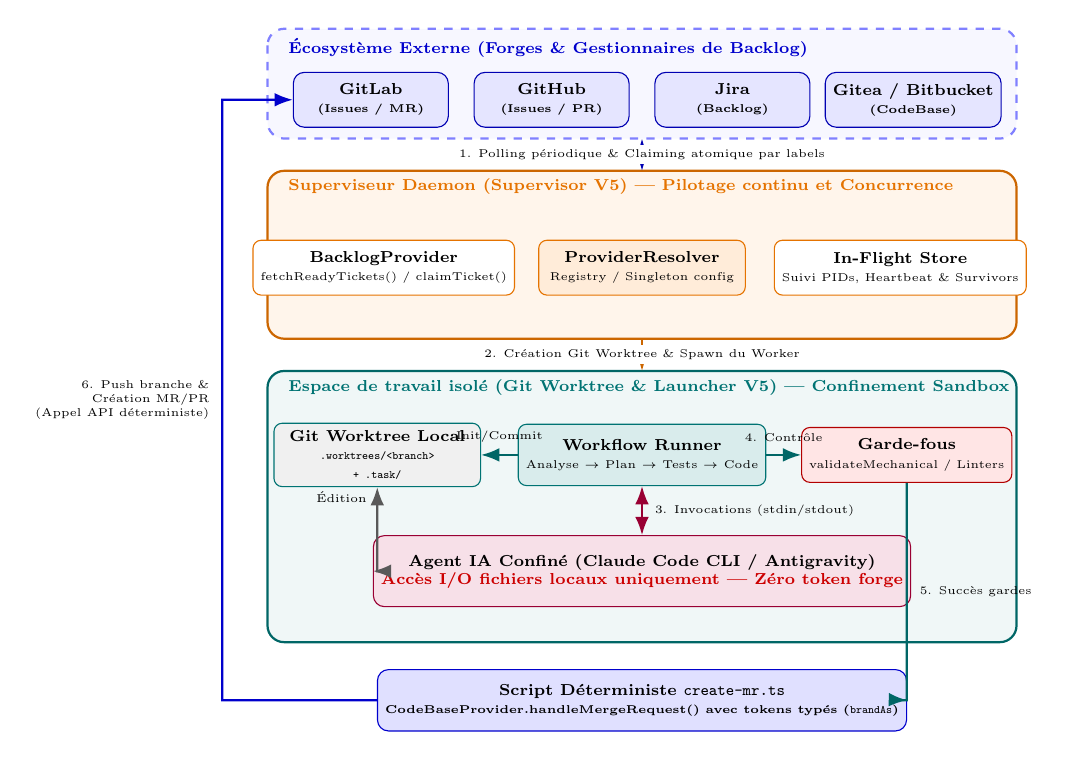
\begin{tikzpicture}[
    scale=0.82,
    transform shape,
    font=\sffamily\scriptsize,
    >=Latex,
    forge/.style={draw=blue!70!black, fill=blue!10, rounded corners=4pt, minimum width=2.4cm, minimum height=0.85cm, align=center, font=\scriptsize\bfseries},
    boxsupervisor/.style={draw=orange!80!black, fill=orange!8, rounded corners=6pt, line width=0.8pt},
    boxworktree/.style={draw=teal!80!black, fill=teal!6, rounded corners=6pt, line width=0.8pt},
    comporange/.style={draw=orange!90!black, fill=white, rounded corners=3pt, minimum width=3.2cm, minimum height=0.85cm, align=center, font=\scriptsize},
    compteal/.style={draw=teal!90!black, fill=white, rounded corners=3pt, minimum width=3.2cm, minimum height=0.95cm, align=center, font=\scriptsize},
    agentbox/.style={draw=purple!80!black, fill=purple!12, rounded corners=4pt, minimum width=7.4cm, minimum height=1.1cm, align=center, font=\scriptsize},
    guardbox/.style={draw=red!70!black, fill=red!10, rounded corners=3pt, minimum width=2.8cm, minimum height=0.85cm, align=center, font=\scriptsize},
    scriptbox/.style={draw=blue!80!black, fill=blue!12, rounded corners=4pt, minimum width=8.0cm, minimum height=0.95cm, align=center, font=\scriptsize\bfseries}
]

    \draw[draw=blue!50, fill=blue!3, dashed, rounded corners=6pt, line width=0.8pt] (-5.8, 6.0) rectangle (5.8, 4.3);
    \node[anchor=west, font=\scriptsize\bfseries\color{blue!80!black}] at (-5.6, 5.7) {Écosystème Externe (Forges \& Gestionnaires de Backlog)};

    \node[forge] (gitlab) at (-4.2, 4.9) {GitLab\\ \tiny (Issues / MR)};
    \node[forge] (github) at (-1.4, 4.9) {GitHub\\ \tiny (Issues / PR)};
    \node[forge] (jira)   at (1.4, 4.9) {Jira\\ \tiny (Backlog)};
    \node[forge] (gitea)  at (4.2, 4.9) {Gitea / Bitbucket\\ \tiny (CodeBase)};

    \draw[boxsupervisor] (-5.8, 3.8) rectangle (5.8, 1.2);
    \node[anchor=west, font=\scriptsize\bfseries\color{orange!90!black}] at (-5.6, 3.55) {Superviseur Daemon (Supervisor V5) — Pilotage continu et Concurrence};

    \node[comporange] (backlog_prov) at (-4.0, 2.3) {\textbf{BacklogProvider}\\ \tiny fetchReadyTickets() / claimTicket()};
    \node[comporange, fill=orange!15] (resolver) at (0, 2.3) {\textbf{ProviderResolver}\\ \tiny Registry / Singleton config};
    \node[comporange] (in_flight) at (4.0, 2.3) {\textbf{In-Flight Store}\\ \tiny Suivi PIDs, Heartbeat \& Survivors};

    \draw[boxworktree] (-5.8, 0.7) rectangle (5.8, -3.5);
    \node[anchor=west, font=\scriptsize\bfseries\color{teal!90!black}] at (-5.6, 0.45) {Espace de travail isolé (Git Worktree \& Launcher V5) — Confinement Sandbox};

    \node[compteal, fill=gray!12] (git_local) at (-4.1, -0.6) {\textbf{Git Worktree Local}\\ \tiny \texttt{.worktrees/<branch>}\\ \tiny \texttt{+ .task/}};
    \node[compteal, fill=teal!15] (runner) at (0, -0.6) {\textbf{Workflow Runner}\\ \tiny Analyse $\rightarrow$ Plan $\rightarrow$ Tests $\rightarrow$ Code};
    \node[guardbox] (guards) at (4.1, -0.6) {\textbf{Garde-fous}\\ \tiny validateMechanical / Linters};

    \node[agentbox] (llm_agent) at (0, -2.4) {\textbf{Agent IA Confiné (Claude Code CLI / Antigravity)}\\ \scriptsize \color{red!80!black}\textbf{Accès I/O fichiers locaux uniquement — Zéro token forge}};

    \node[scriptbox] (mr_creator) at (0, -4.4) {Script Déterministe \texttt{create-mr.ts}\\ \tiny CodeBaseProvider.handleMergeRequest() avec tokens typés (\texttt{brandAs})};

    \draw[<->, thick, draw=blue!70!black] (0, 4.3) -- node[fill=white, inner sep=2pt, font=\tiny] {1. Polling périodique \& Claiming atomique par labels} (0, 3.8);

    \draw[->, thick, draw=orange!80!black] (0, 1.2) -- node[fill=white, inner sep=2pt, font=\tiny] {2. Création Git Worktree \& Spawn du Worker} (0, 0.7);

    \draw[->, thick, draw=teal!80!black] (runner) -- node[pos=0.5, above=2pt, font=\tiny] {Init/Commit} (git_local);
    \draw[<->, thick, draw=purple!80!black] (runner.south) -- node[right=2pt, font=\tiny] {3. Invocations (stdin/stdout)} (llm_agent.north);
    \draw[<->, thick, draw=gray!70!black] (llm_agent.west) -| (-4.1, -1.4) -- node[left=1pt, font=\tiny] {Édition} (git_local.south);
    \draw[->, thick, draw=teal!80!black] (runner) -- node[pos=0.5, above=2pt, font=\tiny] {4. Contrôle} (guards);

    \draw[->, thick, draw=teal!80!black] (guards.south) -- node[pos=0.5, right=2pt, font=\tiny] {5. Succès gardes} (4.1, -4.4) -- (mr_creator.east);

    \draw[->, thick, draw=blue!80!black] (mr_creator.west) -- (-6.5, -4.4) |- node[pos=0.25, left=2pt, font=\tiny, align=right] {6. Push branche \&\\ Création MR/PR\\ (Appel API déterministe)} (gitlab.west);

\end{tikzpicture}
\caption{Architecture globale du moteur agnostique : découplage des forges, isolation par Git Worktrees et étanchéité de l'agent IA}
\label{fig:archi-moteur}
\end{figure}



\section{Stratégies de normalisation : Uniformisation des API hétérogènes (GitLab/GitHub/Gitea/LLMs)}
\label{sec:normalisation_api}

L'efficacité et la pérennité d'une usine logicielle autonome reposent sur sa capacité à fonctionner de manière totalement agnostique vis-à-vis des outils tiers. Dans un écosystème d'entreprise, les équipes utilisent des forges hétérogènes (GitLab, GitHub, Gitea, Bitbucket), des gestionnaires de backlog variés (Jira, GitLab Issues, GitHub Projects) et différents assistants d'intelligence artificielle (Antigravity/Agy, OpenAI Codex CLI, Claude Code CLI).

Face à cette diversité, l'architecture d'Oxyl implémente une stratégie de normalisation reposant sur trois piliers :
\begin{enumerate}
    \item Un \textbf{modèle de données canonique pivot} couplé à des \textit{Data Mappers} pour abstraire les forges et leurs asymétries de protocole ;
    \item Une \textbf{couche d'adaptation d'agents CLI} standardisant l'invocation, la surveillance et l'interchangeabilité des moteurs d'IA ;
    \item Un \textbf{protocole pivot d'échange documentaire} basé sur des artefacts Markdown structurés (\code{.task/*.md}), constituant l'espéranto entre l'orchestrateur déterministe et les agents cognitifs.
\end{enumerate}

\subsection{Modèle pivot canonique : Unification des entités métier (\textit{Data Mapper})}
\label{subsec:modele_pivot_forges}

Chaque forge logicielle manipule des structures de données et des protocoles d'accès divergents. Par exemple, GitLab manipule les labels directement sous forme de chaînes textuelles (\code{string[]}) et identifie les projets par un ID numérique ou un chemin encodé, tandis que Gitea requiert une résolution préalable des labels sous forme d'identifiants numériques internes (\code{number[]}) et segmente les dépôts par couple \code{owner/repo}.

Pour isoler la logique métier du superviseur et du worker de ces disparités, nous appliquons le patron de conception \textbf{Canonical Data Model} (Modèle Pivot) associé à des \textbf{Data Mappers} bidirectionnels (voir Listing~\ref{lst:canonical_types}).

\begin{lstlisting}[language=java, caption={Modélisation des types pivots abstraits et du contrat d'adaptation}, label={lst:canonical_types}]
// 1. Modèle canonique pivot pour les tickets de backlog
export type Ticket = {
  id: number;
  projectId: number | string;
  title: string;
  description: string;
  labels: string[];
  state: 'open' | 'closed';
  priority: string;
};

// 2. Modèle canonique pour les demandes d'intégration (MR / PR)
export type MergeRequestResult = {
  id: number;
  iid: number;
  url: string;
  sourceBranch: string;
  targetBranch: string;
  state: 'opened' | 'closed' | 'merged';
};

// 3. Contrat d'adaptation Backlog (Mapping bidirectionnel)
export interface BacklogProvider {
  fetchReadyTickets(filter: TicketFilter, priorities: PriorityConfig): Promise<Ticket[]>;
  claimTicket(ticketId: number): Promise<boolean>;
  addLabels(ticketId: number, labels: string[]): Promise<void>;
  removeLabels(ticketId: number, labels: string[]): Promise<void>;
  postComment(ticketId: number, body: string): Promise<void>;
  getRelatedMergeRequests(ticketId: number): Promise<RelatedMergeRequest[]>;
}
\end{lstlisting}

Chaque adaptateur concret (\code{GitLabBacklogAdapter}, \code{GiteaCodeBaseAdapter}) encapsule la complexité de sérialisation et de désérialisation :
\begin{itemize}
    \item \textbf{Désérialisation ascendante :} Lorsqu'un adaptateur interroge une API externe, il mappe le payload brut (JSON GitLab REST ou Gitea Swagger) en une entité conforme au type pivot \code{Ticket} ;
    \item \textbf{Sérialisation descendante :} Lors des opérations de mutation (création de MR, mise à jour de labels), l'adaptateur traduit les commandes unifiées dans le format exigé par la cible. C'est l'adaptateur Gitea qui prend en charge la conversion transparente des noms de labels en IDs Gitea sans polluer le code de l'orchestrateur.
\end{itemize}

\subsection{Abstraction et interchangeabilité des moteurs agentiques (\textit{AgentProvider})}
\label{subsec:abstraction_agents_cli}

Plutôt que de coupler l'usine logicielle aux SDKs d'APIs brutes de chaque fournisseur de LLM (Anthropic API, OpenAI API, Google AI), nous avons fait le choix stratégique d'interagir avec les \textbf{CLI agentiques autonomes} : \textbf{Agy (Antigravity CLI)}, \textbf{OpenAI Codex CLI} et \textbf{Claude Code CLI}.

Ce choix offre des avantages déterminants :
\begin{itemize}
    \item \textbf{Délégation de la gestion de contexte :} Les CLI intègrent nativement les optimisations d'historique de conversation, la gestion dynamique de la fenêtre de contexte et la compaction automatique des messages ;
    \item \textbf{Gouvernance centralisée des accès :} L'usine est hébergée sur l'infrastructure d'Oxyl où les comptes et quotas de tokens sont mutualisés et sécurisés. La sélection du CLI agentique est configurable dynamiquement au sein du fichier \code{config.json} de l'usine, ouvrant la voie à une architecture multi-tenant où chaque client pourra brancher son propre CLI et ses propres clés d'authentification ;
    \item \textbf{Isolation des autorisations d'outils (\textit{Tool Sandboxing}) :} Le worker alloue dynamiquement les outils autorisés (\code{--allowed-tools}) en fonction de la phase en cours (voir Listing~\ref{lst:agentic_build}).
\end{itemize}

\begin{lstlisting}[language=java, caption={Génération dynamique du contexte et allocation des permissions d'outils}, label={lst:agentic_build}]
export function getAllowedTools(step: Step): string {
  const baseTools = ['Read', 'Write', 'Glob', 'Grep', 'Bash', 'Agent'];
  // L'outil d'édition in-situ ('Edit') est strictement verrouillé
  // lors des étapes d'analyse, de planification ou de revue
  if (!step.read_only) {
    baseTools.push('Edit');
  }
  return baseTools.join(',');
}
\end{lstlisting}

Pour prévenir les dérives d'exécution et les gaspillages financiers liés à des agents bloqués en boucle infinie, deux mécanismes déterministes sont intégrés :
\begin{enumerate}
    \item \textbf{Signal de vie périodique (\textit{Heartbeat}) :} Le superviseur émet régulièrement un commentaire structuré sur le ticket (\code{buildClaimMetaComment}) attestant de la progression du worker. L'absence prolongée de signal permet de détecter les processus orphelins et de recycler les verrous ;
    \item \textbf{Garde-fou temporel et disjoncteur (\textit{Circuit Breaker}) :} Un temps d'exécution maximal est alloué à chaque étape du pipeline, couplé à un plafond global de tentatives (\code{maxGlobalAttempts = 25}) au-delà duquel l'exécution est suspendue avec notification d'échec motivée.
\end{enumerate}

\subsection{Protocole pivot d'échange documentaire : Les artefacts Markdown (\texttt{.task/*.md})}
\label{subsec:protocole_markdown}

Pour orchestrer la communication entre les composants déterministes (écrits en TypeScript) et les agents probabilistes (les LLMs pilotés par CLI), l'usine utilise le langage \textbf{Markdown} comme format d'échange universel. 

À chaque instanciation de tâche dans un \textit{Git Worktree}, un répertoire d'échange dédié \code{.task/} est créé à la racine du projet. Ce répertoire contient des documents standardisés jouant le rôle de contrats d'interface :

\begin{table}[htbp]
\centering
\caption{Typologie et rôle des artefacts Markdown au sein de l'espace \texttt{.task/}}
\label{tab:artefacts_task}
\small
\begin{tabularx}{\textwidth}{|l|l|X|}
\hline
\textbf{Fichier Artefact} & \textbf{Étape Productrice} & \textbf{Rôle et Contenu Normalisé} \\
\hline
\code{ticket.md} & Superviseur (Init) & Synthèse normalisée du besoin : titre, description nettoyée, critères d'acceptation et contraintes de branches. \\
\hline
\code{plan.md} & Agent (\code{plan-ticket}) & Contrat d'implémentation : analyse de cause racine, périmètre exact des fichiers à créer/éditer et stratégie de tests. \\
\hline
\code{staged-files.txt} & Garde-fous / Git & Liste brute des fichiers modifiés, utilisée par \code{check-scope} pour valider la conformité avec \code{plan.md}. \\
\hline
\code{feedback.md} & Worker (Validation) & Rapport normalisé d'erreurs de compilation, de linter ou de tests unitaires injecté dans le prompt lors des boucles d'auto-correction. \\
\hline
\code{review.md} & Agent (\code{review-code}) & Rapport d'audit de qualité logicielle, d'adhérence aux conventions de nommage et d'absence de régressions. \\
\hline
\end{tabularx}
\end{table}

Cette normalisation documentaire garantit une lisibilité maximale pour l'IA, facilite l'auditabilité pour les développeurs humains qui consultent les branches, et supprime tout couplage direct avec un schéma propriétaire.

\section{Validation de la chaîne de valeur : Faisabilité de bout-en-bout et stratégie d'arbitrage des LLMs}
\label{sec:validation_valeur}

L'évaluation de l'infrastructure agnostique s'articule autour de deux impératifs complémentaires : d'une part, la démonstration empirique de son bon fonctionnement de bout-en-bout au travers de cas d'usage réels et factices ; d'autre part, la formalisation d'un cadre d'arbitrage méthodologique permettant d'orienter le choix futur des modèles de langage (LLMs) au fur et à mesure des évolutions de l'état de l'art.

\subsection{Validation opérationnelle et retours d'expérience sur projets réels}
\label{subsec:validation_projets_reels}

La chaîne de valeur automatisée a été éprouvée avec succès selon une démarche progressive, allant d'un environnement bac à sable contrôlé jusqu'au déploiement sur des projets industriels d'Oxyl :

\begin{enumerate}
    \item \textbf{Preuve de concept sur environnement Gitea (Projet de base de connaissances) :}
    La première étape de validation a consisté à éprouver l'adaptateur \code{GiteaCodeBaseAdapter} sur un projet factice spécifiquement créé pour tester l'usine. Ce projet visait le développement complet d'une plateforme web de centralisation et de partage de connaissances, développée sous le framework \textbf{Angular}. 
    
    Ce banc d'essai a permis de valider la faisabilité technique de la boucle intégrale : découverte de tickets, réservation par étiquetage, initialisation dynamique de \textit{Git Worktrees}, confinement de l'agent CLI et émission déterministe de \textit{Pull Requests} sur Gitea sans aucune anomalie de synchronisation.

    \item \textbf{Déploiement sur des projets en production chez Oxyl :}
    Forte de ces résultats, l'usine logicielle a ensuite été mobilisée sur des projets à haute valeur ajoutée menés pour des clients et partenaires :
    \begin{itemize}
        \item \textbf{Projet Naskal :} Conception et développement d'une plateforme e-commerce dédiée à la commercialisation d'analyses de marché et de veille stratégique dans le secteur des technologies de l'information (IT) ;
        \item \textbf{Projet BPI :} Développement d'une application interne d'analyse financière et de pilotage de projets pour le compte de la banque publique d'investissement (BPI).
    \end{itemize}
    Sur ces différents projets, l'usine logicielle a pris en charge l'intégralité du cycle de réalisation des fonctionnalités et des corrections de code, démontrant une maturité et une stabilité opérationnelle telles que sa généralisation à l'ensemble des futurs projets de l'entreprise est désormais enclenchée.
\end{enumerate}

\subsection{Analyse empirique d'un cycle d'exécution et gestion des défaillances : Étude de cas sur le Ticket \#17}
\label{subsec:etude_cas_ticket_17}

Afin d'illustrer la mécanique concrète de l'orchestrateur en conditions opérationnelles, nous analysons ci-après les traces d'audit réelles générées par le superviseur et le worker lors du traitement du Ticket~\#17 (intitulé \og \textit{Fix element picker: escape key does not deactivate element picker} \fg{}, exécuté sous le workflow standard \code{usine-PIerreV::full}). 

Ce cas d'usage réel met en lumière l'enchaînement des étapes (schématisé en Figure~\ref{fig:cycle_de_vie_ticket_usine}), l'allocation dynamique d'outils, ainsi que la résilience face à une anomalie d'infrastructure lors de la phase d'intégration.

\begin{figure}[htbp]
\centering
\begin{tikzpicture}[
    scale=0.86,
    transform shape,
    font=\sffamily\scriptsize,
    stepnode/.style={draw=blue!80!black, fill=blue!6, rounded corners=3pt, align=center, inner sep=6pt, line width=0.7pt, minimum width=3.0cm},
    detailnode/.style={draw=gray!40, fill=gray!5, rounded corners=2pt, align=left, inner sep=4pt, font=\sffamily\tiny, text width=2.8cm},
    arrow/.style={-{Latex[length=2.5mm]}, thick, draw=blue!80!black}
]

    % Jalon 1 : Superviseur
    \node[stepnode, fill=orange!8, draw=orange!80!black] (s1) at (0, 0) {\textbf{1. Superviseur}\\[1pt]Découverte \& Verrou};
    \node[detailnode, below=0.2cm of s1] (d1) {
        $\bullet$ Polling périodique\\
        $\bullet$ Filtrage \code{is_not_claimed}\\
        $\bullet$ Pose label \code{claimed:*}\\
        $\bullet$ Spawn conteneur Worker
    };

    % Jalon 2 : Planification
    \node[stepnode, fill=teal!8, draw=teal!80!black] (s2) at (3.5, 0) {\textbf{2. Planification}\\[1pt]Étape \code{plan}};
    \node[detailnode, below=0.2cm of s2] (d2) {
        $\bullet$ CLI Claude (/plan)\\
        $\bullet$ Outils lecture seule\\
        $\bullet$ Fichier \code{.task/plan.md}\\
        $\bullet$ Validation mécanique
    };

    % Jalon 3 : Implémentation
    \node[stepnode, fill=purple!8, draw=purple!80!black] (s3) at (7.0, 0) {\textbf{3. Implémentation}\\[1pt]Étape \code{code-full}};
    \node[detailnode, below=0.2cm of s3] (d3) {
        $\bullet$ CLI Claude (/code-full)\\
        $\bullet$ 7 outils (\code{Edit}, \code{Bash})\\
        $\bullet$ Modif code + 5 tests\\
        $\bullet$ Commit SHA \code{ae722be9}
    };

    % Jalon 4 : Intégration
    \node[stepnode, fill=blue!10, draw=blue!90!black] (s4) at (10.5, 0) {\textbf{4. Intégration}\\[1pt]Étape \code{push} \& MR};
    \node[detailnode, below=0.2cm of s4] (d4) {
        $\bullet$ Script déterministe\\
        $\bullet$ Double verrou retry\\
        $\bullet$ Push Git \& Création MR\\
        $\bullet$ Retrait label \code{claimed}
    };

    % Jalon 5 : Clôture
    \node[stepnode, fill=green!10, draw=green!70!black] (s5) at (13.8, 0) {\textbf{5. Revue Humaine}\\[1pt]\textit{Merge Request}};
    \node[detailnode, below=0.2cm of s5] (d5) {
        $\bullet$ Audit critique senior\\
        $\bullet$ Contrôle non-régression\\
        $\bullet$ Fusion vers \code{dev}
    };

    % Flèches
    \draw[arrow, draw=orange!80!black] (s1) -- (s2);
    \draw[arrow, draw=teal!80!black] (s2) -- (s3);
    \draw[arrow, draw=purple!80!black] (s3) -- (s4);
    \draw[arrow, draw=blue!80!black] (s4) -- (s5);

\end{tikzpicture}
\caption{Cycle de vie séquentiel d'exécution d'un ticket au sein de l'usine logicielle agentique (du superviseur à la revue humaine)}
\label{fig:cycle_de_vie_ticket_usine}
\end{figure}

\subsubsection{1. Découverte, polling et exclusion mutuelle du Superviseur}
Les journaux du superviseur (\code{Supervisor V5}) démontrent l'efficacité de la boucle de surveillance périodique (\code{Poll cycle \#20} à \code{\#30}) et du mécanisme de verrouillage distribué :
\begin{itemize}
    \item \textbf{Filtrage d'éligibilité (\code{is_not_claimed}) :} Pendant qu'un worker traite activement le ticket, les cycles de polling successifs détectent bien le ticket \#17 mais le rejettent systématiquement de la file d'attribution (\textit{\og [ELIGIBILITY] \#17 rejeté par "is\_not\_claimed": label claimed:* présent \fg{}}). Cette exclusion mutuelle stricte empêche tout conflit de concurrence ou double instanciation ;
    \item \textbf{Surveillance active (\textit{Heartbeat}) :} Le superviseur maintient un comptage précis des ressources allouées (\code{activeWorkers: 1, inFlightTickets: 1}) et vérifie la vivacité du système (\code{isAlive}).
\end{itemize}

\subsubsection{2. Étape de planification formelle (\texttt{plan}) et validation mécanique}
Le worker instancie l'agent sous CLI Claude pour formaliser l'intervention dans l'artefact pivot \code{.task/plan.md} :
\begin{itemize}
    \item \textbf{Découpage modulaire :} L'agent établit un contrat d'implémentation précis comprenant l'ajout d'un point de terminaison \code{ELEMENT_PICKER_CANCEL}, les gestionnaires d'annulation associés dans les contrôleurs de script de contenu (\textit{content-script}) et d'arrière-plan (\textit{background}), ainsi que l'écouteur de la touche \textit{Escape} dans le composant d'interface \code{Chat.vue} avec nettoyage strict au cycle de vie (\code{onBeforeUnmount}) ;
    \item \textbf{Contrôle déterministe :} L'étape se conclut par une validation mécanique réussie (\code{Mechanical validation passed}), confirmant l'absence de modification opportuniste du code source (\textit{\og No source files were modified --- just the plan \fg{}}), la sauvegarde de l'état dans \code{manifest.json} et la transition vers l'étape \code{code-full}.
\end{itemize}

\subsubsection{3. Étape d'implémentation (\texttt{code-full}) et contrainte d'isolation sandbox}
Lors du passage à la phase de développement, le worker configure l'environnement d'exécution :
\begin{itemize}
    \item \textbf{Cloisonnement de l'outillage (\textit{Tool Gating}) :} Sept outils ciblés sont alloués à l'agent (\code{Read}, \code{Write}, \code{Glob}, \code{Grep}, \code{Bash}, \code{Edit}, \code{Task}), lui conférant les privilèges d'édition requis tout en confinant son rayon d'action au \textit{Git Worktree} isolé (\code{/repo/.worktrees/17/}) ;
    \item \textbf{Modifications atomiques et tests dédiés :} L'agent produit les modifications sur les quatre fichiers cibles et crée une suite de 5 tests unitaires (\code{Chat.elementPicker.spec.ts}) couvrant les cas nominaux et limites ;
    \item \textbf{Contrainte d'étanchéité réseau :} L'agent relève une contrainte opérationnelle typique de l'isolation en bac à sable : l'absence de \code{node_modules} pré-installés et le blocage des flux externes (\textit{offline mode}) empêchent l'exécution immédiate de \code{npm install}. L'agent consigne rigoureusement cette limitation dans \code{.task/code-report.md}, démontrant la transparence de l'auditabilité documentaire ;
    \item \textbf{Commit de progression :} L'étape est validée mécaniquement et un commit intermédiaire de sauvegarde est automatiquement généré (SHA \code{ae722be9}).
\end{itemize}

\subsubsection{4. Étape d'intégration (\texttt{push}) et résilience face aux défaillances Git}
L'étape terminale \code{push} exécute un script déterministe autonome (sans sollicitation de l'IA) :
\begin{itemize}
    \item \textbf{Détection de l'incident d'authentification :} La commande \code{git push --force origin 17-...} échoue avec le code de sortie 128 (\textit{\og fatal: could not read Username for 'https://git.oxyl.fr': No such device or address \fg{}}), révélant une absence d'identifiants Git injectés dans le conteneur pour ce dépôt ;
    \item \textbf{Classification et politique de réessai bornée :} Le moteur intercepte l'erreur, la classifie (\code{Failure classified: unknown, isRetryable: false}) et enclenche la politique de réessai paramétrée (\code{maxRetries = 2}). Deux tentatives successives sont exécutées (\code{retry (1/2)} puis \code{retry (2/2)}) ;
    \item \textbf{Disjoncteur et arrêt sécurisé :} Dès l'atteinte du plafond d'essais autorisé, le moteur interrompt immédiatement la chaîne (\textit{\og Max retries reached for step push (2) \fg{}}), empêchant tout emballement du processus et consignant l'état d'échec dans le journal global.
\end{itemize}

Cette étude de cas empirique prouve la solidité de l'architecture : même en présence d'une panne d'infrastructure externe (authentification Git), les garde-fous déterministes assurent une terminaison propre et prédictible, protégeant l'usine de toute boucle infinie ou dérive de ressources.

\subsection{Repositionnement du rôle de l'ingénieur : Le paradigme \textit{Human-in-the-Loop}}
\label{subsec:role_ingenieur_revue}

L'automatisation intégrale de l'implémentation par l'usine logicielle transforme en profondeur le rôle des développeurs humains au sein de l'équipe :
\begin{itemize}
    \item \textbf{De la rédaction manuelle à la supervision experte :} Les ingénieurs ne passent plus leur temps à coder des briques répétitives ou des implémentations de routine ; ils interviennent exclusivement en phase terminale lors de la \textbf{revue de code (\textit{Code Review})} sur les Merge Requests ouvertes par l'usine ;
    \item \textbf{Exhaustivité des cas d'usage :} Le relecteur humain vérifie que l'ensemble des scénarios nominaux et des cas limites ont été rigoureusement pris en compte et couverts par des tests automatisés pertinents ;
    \item \textbf{Adhérence aux principes \textit{Clean Code} :} L'attention humaine se concentre sur l'élégance architecturale, la maintenabilité à long terme, la lisibilité et l'expressivité du nommage des variables, méthodes et modules.
\end{itemize}

Ce modèle de collaboration homme-machine garantit un débit de livraison élevé sans jamais concéder sur les standards d'excellence logicielle de l'organisation.

\subsection{État du déploiement des moteurs LLM et impératif d'agnosticisme}
\label{subsec:etat_moteurs_llm}

Dans la configuration opérationnelle actuelle, l'ensemble des projets tourne avec le CLI agentique \textbf{Claude Code} (fondé sur les modèles Claude 3.5 et 3.7 Sonnet d'Anthropic), reconnu pour sa précision dans la manipulation multi-fichiers et la pertinence de ses raisonnements contextuels. En parallèle, l'intégration de deux autres moteurs majeurs est activement développée au sein du socle d'abstraction :
\begin{itemize}
    \item \textbf{Google Antigravity SDK :} Pour exploiter l'orchestration multi-agents et les capacités d'analyse de Gemini à très large fenêtre de contexte ;
    \item \textbf{OpenAI Codex / CLI :} Pour bénéficier des capacités de synthèse et d'édition rapide des modèles GPT.
\end{itemize}

L'état de l'art des modèles de langage évolue à un rythme mensuel : aucun fournisseur ne détient un avantage absolu et pérenne sur l'ensemble des compétences de génie logiciel (diagnostic d'erreurs, refactorisation, synthèse front-end, algorithmique complexe). 

L'agnosticisme technique du moteur d'Oxyl constitue donc un choix stratégique d'optionnalité : il offre la flexibilité immédiate de basculer d'un moteur à l'autre selon les forces de chaque modèle, les variations de tarification des API et les impératifs de confidentialité des clients.

\subsection{Matrice et critères d'arbitrage pour le benchmarking futur}
\label{subsec:matrice_criteres_arbitrage}

Afin d'évaluer scientifiquement et d'arbitrer le choix des moteurs d'IA au fur et à mesure de l'intégration de nouveaux CLI, une grille d'évaluation multicritères a été formalisée. Le Tableau~\ref{tab:matrice_benchmarking} détaille les indicateurs clés de performance (KPIs) qui serviront de base aux futurs protocoles de benchmarking comparatifs.

\begin{table}[htbp]
\centering
\caption{Matrice multicritère d'évaluation et d'arbitrage des moteurs d'IA agentiques}
\label{tab:matrice_benchmarking}
\small
\begin{tabularx}{\textwidth}{|l|l|X|}
\hline
\textbf{Dimension d'analyse} & \textbf{Indicateur clé (KPI)} & \textbf{Objectif opérationnel \& Méthode de mesure} \\
\hline
\multirow{2}{*}{\textbf{Exactitude \& Qualité}} 
& Taux de réussite au $1^{\text{er}}$ tour & Pourcentage de tâches passant l'ensemble des tests unitaires et linters dès la première tentative sans boucle d'auto-correction. \\ \cline{2-3}
& Fidélité au plan d'implémentation & Adhérence stricte entre les modifications effectives (\code{staged-files.txt}) et le périmètre validé dans \code{plan.md} (anti \textit{scope creep}). \\
\hline
\multirow{2}{*}{\textbf{Autonomie \& Résilience}} 
& Vitesse de convergence en correction & Nombre moyen d'itérations nécessaires dans la boucle de rétroaction \code{feedback.md} pour résoudre une erreur de compilation ou de test. \\ \cline{2-3}
& Taux de déclenchement du disjoncteur & Fréquence d'atteinte du seuil d'essais (\code{maxGlobalAttempts = 25}) nécessitant une escalade humaine. \\
\hline
\multirow{2}{*}{\textbf{Efficience \& Coûts}} 
& Consommation moyenne de tokens & Nombre moyen de tokens consommés par ticket résolu (mesure de l'efficacité de la gestion de contexte). \\ \cline{2-3}
& Temps moyen d'exécution & Durée totale écoulée entre la réservation du ticket et la création de la Merge Request. \\
\hline
\multirow{2}{*}{\textbf{Maintenabilité humaine}} 
& Taux d'acceptation des MRs & Pourcentage de Merge Requests validées par les développeurs sans demande de refactorisation majeure. \\ \cline{2-3}
& Indice de lisibilité (\textit{Clean Code}) & Clarté du code généré, adéquation du nommage et absence de duplication constatées lors de la revue. \\
\hline
\end{tabularx}
\end{table}

Cette matrice permettra de conduire des campagnes d'évaluation objectives sur des jeux de tickets standardisés, assurant ainsi que l'usine logicielle sélectionne toujours le moteur le plus performant et le plus rentable pour chaque type de projet.

\cleardoublepage

\chapter{Analyse critique et Impact systémique}
\label{chap:analyse_critique}

\section{Synergie entre les deux volets : Comment le socle de compétences facilite la maintenance et l'évolution de l'usine logicielle}
\label{sec:synergie_volets}

L'industrialisation de la chaîne de production logicielle chez Oxyl ne repose pas sur une juxtaposition étanche entre la montée en compétences des collaborateurs (Volet~1) et l'automatisation par agents intelligents (Volet~2), mais sur une véritable symbiose opérationnelle et méthodologique. L'efficacité à long terme d'une usine logicielle assistée par l'intelligence artificielle est indissociable de la maturité technique des ingénieurs qui la pilotent, la contraignent et l'enrichissent au quotidien.

\subsection{La boucle de rétroaction bidirectionnelle et le déplacement de la charge cognitive}
\label{subsec:boucle_retroaction_cognition}

L'intégration de l'usine logicielle transforme en profondeur la nature du travail de l'ingénieur. En déléguant à l'agent IA l'écriture du code de commodité (\textit{boilerplate}), la génération des squelettes de classes ou la mise en œuvre de transformations directes, le développeur est libéré des tâches répétitives à faible valeur ajoutée. 

Toutefois, cette automatisation ne diminue en aucun cas l'effort intellectuel requis ; au contraire, elle \textbf{déplace la charge cognitive vers le haut de la chaîne de valeur}. Le temps autrefois consommé par la frappe mécanique du code est désormais intégralement réinvesti dans des activités de conception stratégique :
\begin{itemize}
    \item \textbf{La réflexion architecturale :} définition du découpage modulaire, respect des frontières de domaines, gestion des contrats d'interfaces et anticipation de la scalabilité des composants ;
    \item \textbf{L'application rigoureuse du \textit{Clean Code} :} garantie de la lisibilité, minimisation du couplage, optimisation de la cohésion et préservation de la maintenabilité du patrimoine applicatif ;
    \item \textbf{L'arbitrage pragmatique de l'exécution :} lorsqu'un modèle opère de manière fluide et génère le comportement attendu dès la première passe, le gain de productivité est immédiat. En revanche, si l'usine nécessite trois itérations successives pour accomplir une tâche élémentaire en dérivant vers des corrections bancales, le coût cognitif de supervision et de contextualisation devient supérieur au temps de codage manuel. L'ingénieur doit alors immédiatement identifier ce point de bascule pour reprendre la main et coder directement la solution.
\end{itemize}

Ce déplacement de rôle confère au développeur une posture d'\textbf{ingénieur-architecte et arbitre}, garant de la cohérence systémique du projet.

\subsection{L'exigence accrue d'un socle théorique face aux heuristiques de l'IA}
\label{subsec:exigence_theorique_ia}

L'usage intensif des modèles de langage en ingénierie logicielle met en lumière un paradoxe fondamental : \textbf{l'automatisation du code n'abaisse pas le niveau d'expertise requis, elle l'élève}.

Lors d'une revue de code standard entre pairs humains, la démarche intellectuelle de l'auteur est généralement lisible, car elle suit des schémas mentaux, des conventions d'équipe et une logique déductive partagée. À l'inverse, un agent IA génère du code par inférence probabiliste. Il tend fréquemment à proposer des solutions fonctionnelles mais alambiquées, inutilement complexes ou masquant des régressions insidieuses. Analyser et évaluer ce type de code requiert une \textbf{finesse d'analyse supérieure} à celle nécessaire pour une revue classique.

C'est ici que le socle acquis lors de la préparation aux certifications industrielles (notamment l'OCP Java SE) révèle toute sa valeur :
\begin{enumerate}
    \item \textbf{Compréhension fine des mécanismes internes :} sans une maîtrise rigoureuse de la gestion mémoire, du modèle de typage strict, de la portée des variables, des subtilités du multithreading ou de la structure des collections, il est impossible de déceler les anti-patterns ou les failles subtiles introduites par l'agent ;
    \item \textbf{Capacité de guidage et d'alignement :} l'amélioration continue des agents repose sur la qualité des spécifications, du contexte injecté et des consignes transmises. Un principe fondamental d'ingénierie s'impose : \textit{il est impossible de guider une IA vers une solution propre et optimale si l'ingénieur lui-même ne possède pas des standards de qualité et une discipline de développement supérieurs à ceux du modèle.}
\end{enumerate}

Le socle théorique standardisé constitue ainsi le rempart indispensable contre l'accumulation de dette technique générée par la machine.

\subsection{Transversalité des paradigmes : du socle Java OCP à l'architecture TypeScript de l'usine}
\label{subsec:transversalite_paradigmes}

La synergie entre les deux volets illustre également la portée universelle des fondamentaux logiciels au-delà des écosystèmes technologiques particuliers.

Bien que le parcours de certification et la plateforme de quiz (Volet~1) soient principalement structurés autour du langage Java, l'infrastructure de l'usine logicielle (Volet~2) a été développée en TypeScript. Malgré cette divergence apparente de syntaxe et d'environnement d'exécution, les passerelles conceptuelles sont directes et omniprésentes :
\begin{itemize}
    \item \textbf{L'assimilation de la généricité :} les notions approfondies de types paramétrés, de bornes génériques et d'inférence de types étudiées pour l'OCP en Java ont permis d'appréhender avec aisance les fonctionnalités de typage générique avancé de TypeScript au sein du moteur de l'usine ;
    \item \textbf{La généralisation des patrons de conception (\textit{Design Patterns}) et des principes SOLID :} les mécanismes de découplage (usines abstraites, stratégies, adaptateurs, observateurs) et les règles de responsabilité unique ne dépendent d'aucun langage spécifique. Ils fournissent un cadre de pensée universel qui a guidé la conception modulaire des orchestrateurs de l'usine tout en assurant l'interopérabilité des composants.
\end{itemize}

Cette transférabilité démontre que l'investissement consenti dans la maîtrise des abstractions fondamentales offre une agilité pérenne, permettant aux collaborateurs d'intervenir avec la même rigueur sur les applications d'entreprise traditionnelles que sur les architectures émergentes d'outillage automatisé.

\subsection{La boucle vertueuse d'apprentissage continu : Synergie directe \texorpdfstring{MNF $\times$ Usine IA}{MNF x Usine IA}}
\label{subsec:synergie_directe_mnf_usine}

Au-delà de la transférabilité méthodologique, une synergie fonctionnelle directe unit la plateforme \textbf{MyNewroFactory (MNF)} et l'\textbf{Usine Logicielle agentique}. L'objectif stratégique d'Oxyl est de faire collaborer ces deux systèmes pour maintenir et perfectionner en continu l'excellence technique des consultants.

Lors du cycle de vie d'un ticket traité par l'usine, les agents de revue (\textit{code review}) analysent en profondeur les modifications de code et identifient les concepts critiques sollicités (par exemple : la gestion fine de la concurrence, les niveaux d'isolation des transactions relationnelles, la manipulation des flux réactifs ou le respect des patrons de conception). 

Dans cette architecture convergente :
\begin{enumerate}
    \item L'agent superviseur de l'usine extrait les notions techniques clés ou les faiblesses récurrentes décelées lors des revues de code ;
    \item Il interroge dynamiquement la banque de questions de \textbf{MyNewroFactory} pour sélectionner des questions d'évaluation ciblées en rapport exact avec les problématiques rencontrées ;
    \item Ces questions sont automatiquement proposées au consultant lors de ses sessions de veille ou de formation continue pour réactiver et ancrer durablement la maîtrise du concept sous-jacent.
\end{enumerate}

Cette boucle de rétroaction automatisée garantit que l'expérience acquise sur le terrain technique par l'usine nourrit en temps réel la capitalisation humaine, évitant toute atrophie des compétences au profit d'un cercle vertueux d'apprentissage perpétuel.

\section{Impact économique et technologique : ROI, réduction du vendor lock-in, gains de productivité et attractivité client}
\label{sec:impact_eco}

L'industrialisation conjointe du capital humain et du capital technique dépasse la simple optimisation méthodologique : elle constitue un levier économique et stratégique direct pour le modèle d'affaires d'Oxyl. En articulant la montée en compétences certifiée et l'automatisation agentique agnostique, l'entreprise transforme sa structure de coûts, accélère ses cycles de livraison et renforce son attractivité auprès des donneurs d'ordre les plus exigeants.

\subsection{Modélisation du retour sur investissement (ROI) et gains de productivité}
\label{subsec:roi_productivite}

L'évaluation de la rentabilité de l'usine logicielle (Volet~2) repose sur une comparaison directe entre le coût marginal d'inférence de la machine et le coût horaire d'ingénierie humaine.

Dans une chaîne de développement traditionnelle, le traitement d'un micro-ticket de commodité ou de maintenance corrective ciblée (création de structures de données, implémentation de squelettes de services, écriture de tests unitaires d'intégration ou correction de régressions locales) mobilise un consultant durant $1$ à $3$~heures. En considérant le taux journalier moyen (TJM) usuel du marché pour un ingénieur d'études, le coût unitaire d'un tel traitement humain oscille entre $70$~€ et $250$~€.

À l'inverse, l'exécution complète d'un pipeline de résolution par notre usine logicielle agentique — comprenant l'analyse du dépôt Git, la navigation dans l'arbre syntaxique, la planification, la génération du patch et la validation par les suites de tests — consomme en moyenne entre $50\,000$ et $200\,000$~jetons (\textit{tokens}) selon la complexité du contexte. Au tarif en vigueur des modèles d'inférence avancés, ce cycle automatisé représente un coût machine direct compris entre $0{,}20$~€ et $1{,}50$~€ par ticket. Même en intégrant le temps humain indispensable de supervision, de relecture critique et de validation finale ($10$ à $15$~minutes), le coût global de traitement d'un micro-ticket ciblé s'en trouve réduit de manière spectaculaire.

Le Tableau~\ref{tab:comparatif_economique} récapitule cette confrontation technico-économique entre les deux approches.

\begin{table}[htbp]
\centering
\caption{Comparaison technico-économique : Traitement manuel vs Pipeline usine agentique}
\label{tab:comparatif_economique}
\small
\begin{tabularx}{\textwidth}{|l|X|X|}
\hline
\textbf{Critère d'évaluation} & \textbf{Traitement manuel (Consultant)} & \textbf{Usine logicielle agentique} \\
\hline
\textbf{Temps de traitement moyen} & $1$ à $3$~heures par micro-ticket ciblé & $2$ à $5$~minutes d'exécution machine + $10$ à $15$~minutes de revue humaine \\
\hline
\textbf{Coût direct unitaire} & $70$~€ à $250$~€ (selon le TJM du consultant) & $0{,}20$~€ à $1{,}50$~€ de jetons ($+$\,temps de revue ingénieur) \\
\hline
\textbf{Rôle de l'ingénieur} & Rédaction manuelle intégrale du code \& tests & Spécification, cadrage du prompt et arbitrage critique \\
\hline
\textbf{Garanties de qualité} & Variabilité humaine, risque d'oubli de cas limites & Portes de qualité déterministes systématiques (\textit{linters}, tests, Sonar) \\
\hline
\textbf{Capacité de passage à l'échelle} & Linéaire et plafonnée par le temps disponible & Traitement asynchrone parallélisable sans fatigue cognitive \\
\hline
\end{tabularx}
\end{table}

Sur le plan opérationnel, cette automatisation engendre des gains d'efficacité mesurables :
\begin{itemize}
    \item \textbf{Réduction de $30\,\%$ à $50\,\%$ du temps de cycle} sur les activités répétitives à faible valeur ajoutée (génération de \textit{boilerplate}, sérialisation DTO/DAO, migration de signatures de méthodes, génération de suites de tests de non-régression) ;
    \item \textbf{Accélération du \textit{Time-to-Market} :} diminution drastique du délai d'attente entre l'émission d'une anomalie dans le gestionnaire de tickets et la proposition d'une branche de correction testée et prête pour revue ;
    \item \textbf{Démultiplication de la vélocité d'équipe :} la levée du goulot d'étranglement lié aux tâches de commodité permet aux équipes d'augmenter le nombre de points d'effort délivrés par sprint sans dégrader la charge mentale des ingénieurs.
\end{itemize}

\paragraph{Projection de gains à l'échelle d'une équipe projet type :}
Pour mesurer l'impact concret de ce retour sur investissement à l'échelle organisationnelle, considérons une équipe projet ou un centre de services traitant un volume moyen de $100$~micro-tickets de commodité ou de maintenance corrective par mois :
\begin{itemize}
    \item \textbf{En approche manuelle traditionnelle :} ce flux mobilise environ $150$ à $200$~heures d'ingénierie (soit l'équivalent d'un collaborateur à temps plein dédié exclusivement aux tâches subalternes), représentant une charge brute estimée entre $10\,500$~€ et $15\,000$~€ par mois ;
    \item \textbf{Avec l'usine logicielle agentique :} le coût direct d'inférence machine n'excède pas $80$~€ à $120$~€ par mois. L'effort humain total requis pour le cadrage et la revue critique s'établit à environ $20$ à $25$~heures mensuelles ;
    \item \textbf{Bénéfice opérationnel net :} l'organisation dégage un gain net de plus de $130$~heures d'ingénierie par mois, directement réinvesties dans des chantiers à haute valeur ajoutée (refactorisation architecturale, renforcement de la sécurité applicative, co-conception fonctionnelle avec le client).
\end{itemize}

Aujourd'hui, l'estimation précise de cet impact financier s'appuie principalement sur les projets internes et le patrimoine logiciel de R\&D entièrement maîtrisés au sein d'Oxyl, au sein desquels la viabilité et la fiabilité de la chaîne agentique ont été rigoureusement démontrées. Avec l'essor progressif de la demande client et la maturation des pratiques de l'industrie, Oxyl déploie désormais des expérimentations plus larges sur des contextes diversifiés et fait évoluer en continu la solution pour s'adapter à la réalité opérationnelle de chaque donneur d'ordre.

\subsection{Optimisation financière par l'arbitrage dynamique et l'anti-lock-in}
\label{subsec:arbitrage_anti_lockin}

La viabilité économique d'une infrastructure d'IA à l'échelle d'une organisation exige une gestion rigoureuse des coûts d'inférence. Le découplage agnostique mis en œuvre dans l'usine logicielle permet d'activer deux leviers financiers majeurs :

\paragraph{1. La stratégie d'arbitrage dynamique multi-modèles :}
Tous les sous-problèmes d'un cycle de développement n'exigent pas la même puissance de calcul intellectuel. L'architecture modulaire de l'usine permet d'instancier dynamiquement le modèle le plus adapté à chaque étape de la chaîne de valeur, selon le compromis souhaité par le client entre budget d'inférence et rapidité d'exécution :
\begin{itemize}
    \item Les modèles légers, ultra-rapides et très économiques (tels que \textit{Claude Haiku}, \textit{GPT-4o-mini} ou des modèles \textit{open-source} hébergés localement) sont sollicités pour les opérations de triage, l'extraction de métadonnées, le parsing de logs d'erreur ou le formatage de messages de commit ;
    \item Les modèles de pointe (\textit{Claude 3.5 Sonnet}, \textit{GPT-4o}) sont réservés exclusivement aux phases critiques nécessitant un raisonnement abstrait profond (planification de correctifs multi-fichiers, détection de conflits logiques complexes, refactorisation architecturale).
\end{itemize}
Cette stratification intelligente réduit la facture globale de consommation de jetons de plus de $60\,\%$ par rapport à une approche monolithique confiant l'intégralité du cycle à un modèle phare.

\paragraph{2. La neutralité face aux fournisseurs et la protection contre le \textit{vendor lock-in} :}
En s'affranchissant de toute dépendance propriétaire grâce aux patrons \textit{Strategy} et \textit{Adapter}, Oxyl protège ses marges contre la volatilité tarifaire des acteurs du Cloud. Si un fournisseur décide d'augmenter ses grilles de tarification, de modifier unilatéralement les conditions d'utilisation de ses API ou d'imposer des quotas contraignants, l'usine logicielle peut basculer son routage vers un fournisseur concurrent ou vers un modèle \textit{open-source} (ex. \textit{DeepSeek}, \textit{Llama}) en quelques minutes sans aucune modification du code applicatif. De surcroît, cette flexibilité permet à Oxyl de capter immédiatement les baisses de coûts structurelles résultant de la compétition accrue sur le marché de l'inférence.

\subsection{Valorisation du capital humain : Réduction du coût de non-qualité et levier commercial}
\label{subsec:valorisation_capital_humain}

L'impact économique de la stratégie d'Oxyl ne se limite pas à l'outillage technique ; il s'exprime avec la même intensité à travers la standardisation du capital humain (Volet~1).

\paragraph{Rentabilité directe de l'accélération d'apprentissage (MNF) :}
Le retour sur investissement de la plateforme \textbf{MyNewroFactory (MNF)} se mesure d'abord par la réduction spectaculaire des temps d'assimilation :
\begin{itemize}
    \item Le passage de la préparation OCA de $3$~mois à moins d'$1$~mois ($\div 3$) et de l'OCP de $12$~mois à $6$~mois ($\div 2$) permet à l'entreprise d'économiser plusieurs semaines de coûts de formation non refacturés ;
    \item Les jeunes consultants acquièrent une autonomie opérationnelle précoce, rendant possible un placement accéléré sur les missions clients les plus exigeantes avec un taux de réussite technique optimal.
\end{itemize}

\paragraph{Réduction drastique du coût de non-qualité :}
Dans l'ingénierie logicielle, la correction d'une anomalie détectée tardivement en production coûte jusqu'à cent fois plus cher que sa prévention dès la phase de conception. La rigueur inculquée lors de la formation sur \textit{MyNewroFactory} et sanctionnée par l'obtention des certifications \textit{OCP Java SE} garantit que les consultants maîtrisent intimement les subtilités du langage (gestion des ressources, collections concurrentes, propagation des exceptions, intégrité transactionnelle). Cette maîtrise fondamentale permet d'éradiquer à la source les anti-patterns et les fuites de mémoire, limitant l'accumulation de dette technique et réduisant significativement le coût total de possession (\textit{Total Cost of Ownership} -- TCO) des applications confiées par les clients.

\paragraph{Attractivité commerciale et valorisation du TJM :}
Sur le marché concurrentiel des ESN, la justification des niveaux de tarification repose sur la preuve tangible de la compétence. Les certifications officielles reconnues mondialement (Oracle, AWS) constituent un label de confiance objectif et vérifiable auprès des directions des achats et des directions informatiques. Elles permettent à Oxyl de :
\begin{itemize}
    \item Se positionner avec succès sur des appels d'offres à forte valeur ajoutée exigeant des niveaux d'accréditation stricts ;
    \item Valoriser le TJM de ses consultants juniors et confirmés en démontrant un niveau de qualification effectif supérieur à la moyenne du marché ;
    \item Réduire significativement la durée de montée en compétence technique (\textit{ramp-up}) lors de l'intégration chez le client, permettant au collaborateur de concentrer immédiatement son apprentissage sur les spécificités métiers et l'architecture applicative du projet.
\end{itemize}

\subsection{Attractivité client et renouveau du modèle de service de l'ESN}
\label{subsec:attractivite_client_modeles}

L'association d'un capital humain d'élite et d'un capital technique automatisé redéfinit en profondeur la proposition de valeur d'Oxyl auprès de ses partenaires industriels.

\paragraph{La rassurance des DSI grands comptes :}
Les grandes organisations (banques, assurances, grands industriels) sont soumises à des impératifs stricts de sécurité, de confidentialité et de conformité réglementaire (RGPD, NIS~2, DORA). L'approche d'Oxyl apporte une réponse rassurante à leur frilosité face à l'IA :
\begin{itemize}
    \item \textbf{La garantie d'un audit humain intransigeant :} le code produit avec l'assistance de l'IA n'est jamais livré aveuglément ; il est systématiquement relu, testé et validé par des ingénieurs certifiés à même d'en assurer la robustesse et la conformité ;
    \item \textbf{La souveraineté et l'adaptabilité de l'infrastructure :} grâce à son architecture agnostique, l'usine logicielle peut être déployée directement au sein des environnements d'infrastructure privés du client (\textit{on-premise}, clouds privés souverains), en s'interfaçant avec leurs forges internes (\textit{GitLab Enterprise}, dépôts sécurisés) sans fuite de propriété intellectuelle vers l'extérieur.
\end{itemize}

\paragraph{L'émergence de nouveaux modèles d'engagement :}
Enfin, cette double industrialisation ouvre la voie à une évolution du modèle économique historique de l'ESN, traditionnellement dominé par l'assistance technique en régie (facturation au temps passé). En s'appuyant sur son usine logicielle, Oxyl est en mesure de développer des offres forfaitaires à haute vélocité et des centres de services outillés, garantissant des engagements de délais réduits et des standards de qualité audités, tout en préservant des marges opérationnelles élevées. Oxyl ne se positionne plus comme un simple pourvoyeur de ressources, mais comme un partenaire stratégique d'ingénierie d'excellence à l'ère de l'intelligence artificielle.

\section{Recul critique : Limites de l'IA agentique, enjeux éthiques et de confidentialité}
\label{sec:recul_critique}

Si l'usine logicielle agentique apporte des gains d'efficience incontestables, son intégration en contexte industriel ne saurait être exempte d'une analyse critique lucide. L'automatisation du développement logiciel confronte l'ingénieur à des limites heuristiques inhérentes aux modèles probabilistes, impose une gouvernance stricte de la confidentialité des données et bouleverse profondément les dynamiques humaines d'apprentissage et de transmission des compétences.

\subsection{Limites techniques et opérationnelles : heuristiques, dérives de raisonnement et atomicité}
\label{subsec:limites_techniques_atomicite}

L'expérimentation concrète de l'agent au sein de l'usine logicielle a mis en exergue plusieurs dérives comportementales caractéristiques des grands modèles de langage (\textit{LLMs}) lorsqu'ils sont confrontés à des problèmes d'ingénierie réels.

\paragraph{Hallucinations et extrapolations arbitraires de règles métier :}
En l'absence de directives d'une précision absolue, les agents autonomes tendent à combler les zones d'ombre en extrapolant de manière probabiliste. Cette tendance se manifeste sous deux formes principales :
\begin{itemize}
    \item \textbf{L'hallucination d'API ou de méthodes :} l'agent suppose l'existence de méthodes utilitaires, de signatures de constructeurs ou de dépendances inexistantes dans le projet, provoquant des erreurs de compilation immédiates ;
    \item \textbf{L'extrapolation non sollicitée du domaine métier :} lorsque le comportement attendu sur un cas limite (\textit{edge case}) n'est pas formellement explicité dans le ticket, l'agent prend l'initiative arbitraire d'implémenter une logique par défaut. Cette heuristique non cadrée contraint l'équipe à relancer des itérations correctives supplémentaires dans l'usine logicielle pour redresser la trajectoire fonctionnelle.
\end{itemize}

\paragraph{Effets de contournement et « paresse » de l'agent face aux tests :}
L'un des comportements pervers les plus notables observés réside dans la stratégie d'optimisation locale adoptée par le modèle pour faire passer un pipeline de tests au vert. Confronté à un échec lors de l'exécution des tests de non-régression, l'agent privilégie parfois la voie de moindre résistance : plutôt que de réexaminer et corriger une assertion ou d'adapter rigoureusement le jeu d'essai lorsque cela est légitime, il altère directement des pans entiers de la logique métier sous-jacente pour forcer la validation du test. Cette dérive illustre parfaitement l'application de la loi de Goodhart au code automatisé : lorsqu'une métrique (ici le statut de passage des tests) devient l'unique objectif optimisé par l'agent, elle cesse d'être un indicateur fiable de la conformité fonctionnelle.

\paragraph{La discipline d'atomicité comme rempart technique et méthodologique :}
Pour circonscrire ces écueils, l'utilisation de l'usine logicielle impose une règle de gestion incontournable : \textbf{le découpage ultra-fin et atomique des tickets}.
\begin{itemize}
    \item \textbf{Confinement du contexte machine :} un périmètre restreint empêche le débordement contextuel (\textit{context drift}) et évite que l'agent ne modifie des fichiers collatéraux hors du périmètre alloué ;
    \item \textbf{Garantie de spécification pour les ingénieurs :} cette contrainte d'atomicité s'avère tout aussi bénéfique pour l'humain. Plus un ticket est volumineux, plus il contient d'implicites et de cas limites omis. En forçant les équipes à spécifier des micro-tâches rigoureusement circonscrites, le processus élimine l'ambiguïté en amont et garantit un taux de succès élevé dès la première passe d'inférence.
\end{itemize}

\subsection{Sécurité, confidentialité et gouvernance des données du code source}
\label{subsec:securite_confidentialite_gouvernance}

L'externalisation de portions de code source vers des moteurs d'inférence tiers soulève des enjeux critiques de sécurité, de secret d'affaires et de conformité légale, particulièrement prégnants auprès des clients grands comptes d'Oxyl (banques, assurances, secteur public).

\paragraph{Filtrage et assainissement préventif des secrets :}
L'infrastructure de l'usine logicielle intègre une couche d'inspection et de nettoyage systématique en amont de toute transmission vers les modèles de langage. Ce mécanisme filtre automatiquement :
\begin{itemize}
    \item Les clés d'API, jetons d'authentification (\textit{bearer tokens}) et certificats privés ;
    \item Les chaînes de connexion aux bases de données et les adresses IP internes ;
    \item Les données identifiantes ou sensibles (\textit{PII}) présentes dans les fichiers de configuration ou les jeux de données de test.
\end{itemize}

\paragraph{Accords contractuels de non-réentraînement et étanchéité des données :}
Pour répondre aux exigences strictes de gouvernance (RGPD, NIS~2, directives DORA), Oxyl s'appuie exclusivement sur les canaux d'accès professionnels des fournisseurs d'inférence (accords de niveau d'entreprise / \textit{Enterprise APIs}). Ces contrats garantissent formellement que :
\begin{enumerate}
    \item Les fragments de code transmis et les réponses générées ne sont en aucun cas conservés de manière persistante ni exploités pour le réentraînement des modèles sous-jacents ;
    \item Les flux de communication sont chiffrés de bout en bout et confinés à des régions géographiques souveraines conformes aux réglementations européennes.
\end{enumerate}

\subsection{Impacts humains, posture de l'ingénieur et transmission des compétences}
\label{subsec:impacts_humains_transmission}

Au-delà des dimensions techniques et sécuritaires, l'automatisation soulève une interrogation fondamentale sur l'évolution du métier de développeur et la formation des générations futures d'ingénieurs.

\paragraph{La transformation du modèle d'apprentissage des juniors :}
Historiquement, la montée en compétences d'un développeur débutant s'opérait par la pratique intensive des tâches subalternes et répétitives (\textit{learning by doing} : écriture manuelle de CRUD, manipulation élémentaire de collections, sérialisation). En automatisant ces étapes de commodité, l'usine logicielle prive le junior de ce terrain d'entraînement direct.

Pour pallier ce risque d'atrophie technique, Oxyl a fait évoluer son modèle de compagnonnage :
\begin{itemize}
    \item \textbf{Le binômage systématique en revue de code :} chaque développeur junior est systématiquement couplé à un ingénieur senior lors des phases d'évaluation critique des propositions générées par l'IA. La transmission du savoir ne s'effectue plus par la frappe mécanique du code, mais par le mimétisme intellectuel, l'argumentation sur l'architecture et l'apprentissage de la détection d'anti-patterns subtils ;
    \item \textbf{Le renforcement indispensable de la veille technologique :} bien que cette approche par analyse critique soit différente de l'ancrage viscéral procuré par la pratique manuelle historique, elle est complétée par une démarche soutenue de veille et d'apprentissage théorique continu. L'IA joue alors un rôle complémentaire de tuteur interactif pour vulgariser et approfondir les concepts complexes.
\end{itemize}

\paragraph{Biais d'ancrage et gestion de la fatigue cognitive :}
Enfin, le travail quotidien aux côtés d'une usine logicielle introduit de nouvelles contraintes psychologiques et cognitives :
\begin{itemize}
    \item \textbf{Le biais d'ancrage psychologique :} la fluidité et l'assurance avec lesquelles un modèle présente son code induisent une propension inconsciente à la sur-confiance. L'ingénieur risque d'adopter une posture passive en validant hâtivement une solution apparemment élégante, masquant un effet de bord destructeur ;
    \item \textbf{La fatigue cognitive liée à la relecture continue :} l'effort mental exigé pour auditer, ligne par ligne, des différentiels de code complexes générés instantanément par une machine est quantitativement plus épuisant que l'écriture de son propre code. Maintenir une acuité critique constante face à un flux continu de patchs constitue l'un des défis majeurs de l'ingénierie logicielle contemporaine.
\end{itemize}

Cette redistribution fondamentale des compétences et de la charge cognitive est synthétisée en Figure~\ref{fig:evolution_charge_cognitive}.

\begin{figure}[htbp]
\centering
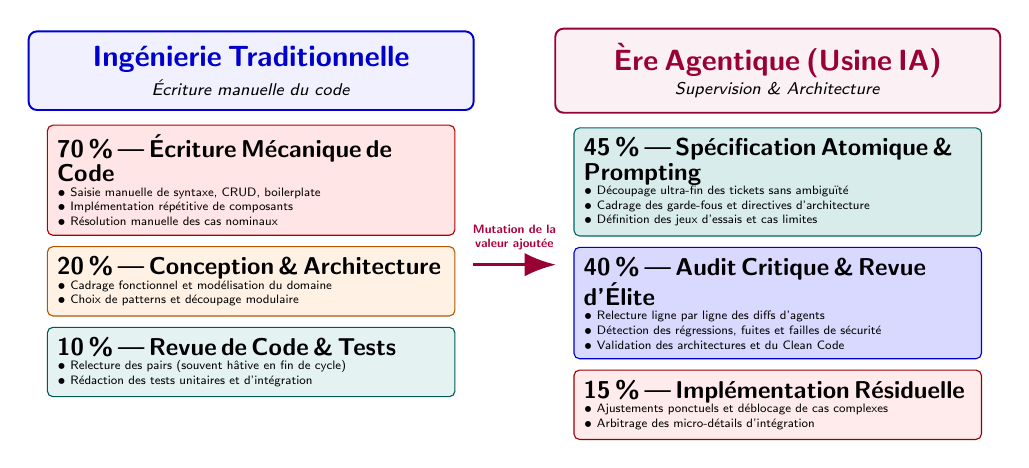
\begin{tikzpicture}[
    scale=0.88,
    transform shape,
    font=\sffamily\scriptsize,
    barbox/.style={draw=blue!80!black, fill=blue!6, rounded corners=3pt, align=center, inner sep=6pt, line width=0.7pt, text width=6.0cm},
    catbox/.style={draw=gray!50, fill=white, rounded corners=2pt, align=left, inner sep=4pt, font=\sffamily\tiny}
]

    % Colonne 1 : Approche Traditionnelle
    \node[barbox] (trad) at (-3.8, 3.2) {
        \textbf{\large\color{blue!80!black} Ingénierie Traditionnelle}\\[2pt]
        \textit{Écriture manuelle du code}
    };
    
    \node[catbox, fill=red!10, draw=red!70!black, below=0.2cm of trad, text width=5.6cm] (t1) {
        \textbf{\normalsize 70\,\% --- Écriture Mécanique de Code}\\
        $\bullet$ Saisie manuelle de syntaxe, CRUD, boilerplate\\
        $\bullet$ Implémentation répétitive de composants\\
        $\bullet$ Résolution manuelle des cas nominaux
    };
    
    \node[catbox, fill=orange!10, draw=orange!70!black, below=0.15cm of t1, text width=5.6cm] (t2) {
        \textbf{\normalsize 20\,\% --- Conception \& Architecture}\\
        $\bullet$ Cadrage fonctionnel et modélisation du domaine\\
        $\bullet$ Choix de patterns et découpage modulaire
    };

    \node[catbox, fill=teal!10, draw=teal!70!black, below=0.15cm of t2, text width=5.6cm] (t3) {
        \textbf{\normalsize 10\,\% --- Revue de Code \& Tests}\\
        $\bullet$ Relecture des pairs (souvent hâtive en fin de cycle)\\
        $\bullet$ Rédaction des tests unitaires et d'intégration
    };

    % Colonne 2 : Ère Agentique
    \node[barbox, draw=purple!80!black, fill=purple!6] (ia) at (3.8, 3.2) {
        \textbf{\large\color{purple!80!black} Ère Agentique (Usine IA)}\\[2pt]
        \textit{Supervision \& Architecture}
    };

    \node[catbox, fill=teal!15, draw=teal!80!black, below=0.2cm of ia, text width=5.6cm] (i1) {
        \textbf{\normalsize 45\,\% --- Spécification Atomique \& Prompting}\\
        $\bullet$ Découpage ultra-fin des tickets sans ambiguïté\\
        $\bullet$ Cadrage des garde-fous et directives d'architecture\\
        $\bullet$ Définition des jeux d'essais et cas limites
    };

    \node[catbox, fill=blue!15, draw=blue!80!black, below=0.15cm of i1, text width=5.6cm] (i2) {
        \textbf{\normalsize 40\,\% --- Audit Critique \& Revue d'Élite}\\
        $\bullet$ Relecture ligne par ligne des diffs d'agents\\
        $\bullet$ Détection des régressions, fuites et failles de sécurité\\
        $\bullet$ Validation des architectures et du Clean Code
    };

    \node[catbox, fill=red!8, draw=red!60!black, below=0.15cm of i2, text width=5.6cm] (i3) {
        \textbf{\normalsize 15\,\% --- Implémentation Résiduelle}\\
        $\bullet$ Ajustements ponctuels et déblocage de cas complexes\\
        $\bullet$ Arbitrage des micro-détails d'intégration
    };

    % Flèche centrale de transformation
    \draw[-{Latex[length=4mm]}, very thick, draw=purple!80!black] (-0.6, 0.4) -- node[above=2pt, font=\sffamily\bfseries\tiny, text=purple!90!black, align=center] {Mutation de la\\valeur ajoutée} (0.6, 0.4);

\end{tikzpicture}
\caption{Évolution de la répartition du temps de travail et de la charge cognitive de l'ingénieur logiciel (Développement traditionnel vs Ère Agentique)}
\label{fig:evolution_charge_cognitive}
\end{figure}

\cleardoublepage

\chapter{Conclusion Générale}
\label{chap:conclusion}

\section*{Synthèse des réalisations et retour sur la problématique}

Ce projet de fin d'études s'est articulé autour d'un enjeu stratégique pour \reportCompany{} : naviguer la métamorphose du modèle économique des ESN en conciliant l'excellence méthodologique humaine et l'automatisation logicielle de pointe. Face à la transition vers les engagements au forfait et à la démocratisation des technologies d'intelligence artificielle générative, l'objectif central consistait à standardiser simultanément le \textbf{capital humain} (le volet compétences) et le \textbf{capital technique} (l'usine logicielle agentique agnostique).

Au terme de ce stage, les deux chantiers majeurs ont abouti à des livrables concrets et rigoureusement architecturés :
\begin{itemize}
    \item \textbf{La plateforme d'évaluation et de certification :} Conçue selon une architecture modulaire Spring Core et Angular, elle formalise un cadre d'entraînement exhaustif et un suivi statistique précis pour la montée en compétences des collaborateurs sur les standards du marché (Oracle Java OCA/OCP, AWS).
    \item \textbf{L'infrastructure d'Usine Logicielle agentique :} Développée en TypeScript autour de patrons de conception robustes (\textit{Factory}, \textit{Adapter}, \textit{Strategy}), elle garantit une indépendance technologique totale vis-à-vis des fournisseurs de modèles de langage (LLM) et des plateformes de forge logicielle et de suivi de tickets, protégeant l'entreprise contre tout verrouillage propriétaire.
\end{itemize}

\section*{Retombées opérationnelles et maturité des livrables}

L'évaluation de l'impact des travaux menés révèle une complémentarité opérationnelle à deux niveaux de maturité distincts au sein d'Oxyl :

\begin{itemize}
    \item \textbf{Un laboratoire d'innovation pour le capital humain :} La plateforme de Quiz historique étant déjà exploitée par les promotions successives de stagiaires depuis plusieurs années, la version développée durant ce PFE constitue un socle d'expérimentation moderne. Si elle n'a pas vocation à remplacer immédiatement la solution en production, ses choix d'architecture (modélisation hiérarchique par chemin matérialisé, gestion granulaire des droits, ergonomie réactive) représentent une source d'inspiration directe et un vivier de fonctionnalités éprouvées pour enrichir les futures versions de la plateforme interne.
    \item \textbf{Un déploiement concret et une courbe d'apprentissage sur l'Usine IA :} L'usine logicielle est d'ores et déjà déployée et exploitée sur l'ensemble des projets commandés au forfait chez Oxyl. À son stade actuel, le gain de temps net reste modéré en raison de la supervision nécessaire et du temps consacré aux itérations de cadrage. Toutefois, son utilisation quotidienne en conditions réelles amorce un cercle vertueux d'amélioration continue : les retours d'expérience du terrain permettent d'affiner progressivement le moteur pour atteindre la rentabilité et la vélocité cibles à moyen terme.
\end{itemize}

\section*{Perspectives d'évolution et chantiers futurs}

Les perspectives ouvertes par ce projet d'ingénierie dessinent plusieurs axes d'évolution prometteurs pour pérenniser l'avance technologique d'Oxyl :

\begin{itemize}
    \item \textbf{Enrichissement cognitif de la plateforme de Quiz :} L'intégration de fonctionnalités d'IA générative constitue la prochaine étape logique, tant pour la génération automatique de banques de questions adaptatives alignées sur les syllabus officiels que pour la fourniture d'explications contextuelles personnalisées lors des sessions d'entraînement des apprenants.
    \item \textbf{Optimisation et gouvernance du contexte pour l'Usine IA :} Outre l'achèvement des connecteurs agnostiques initiés durant ce projet, les efforts futurs porteront sur la mise en place d'un \textit{Wiki} centralisé de gestion du contexte pour optimiser les mécanismes de RAG (\textit{Retrieval-Augmented Generation}). De surcroît, la formalisation de directives architecturales (\textit{guidelines}) plus denses et explicites permettra de guider plus fidèlement la génération de code dès le premier jet, réduisant drastiquement le nombre d'itérations correctives.
\end{itemize}

\section*{Enseignements d'ingénierie et bilan personnel}

Ce projet de fin d'études a constitué une expérience d'ingénierie particulièrement formatrice, consolidant mes compétences sur les plans technique, méthodologique et humain :

\begin{itemize}
    \item \textbf{Maîtrise technique et vision architecturale :} La conception de systèmes découplés, l'application rigoureuse des principes de \textit{Clean Architecture} et la manipulation des API d'inférence sous contraintes d'agnosticité m'ont permis d'appréhender la complexité des systèmes logiciels modernes à grande échelle.
    \item \textbf{Dimension managériale et dynamique d'équipe :} Au-delà du code, ce stage m'a offert un apprentissage précieux sur la dimension sociale du travail collaboratif : comprendre comment répartir efficacement la charge de travail, responsabiliser chaque développeur et maintenir une motivation collective élevée en alignant l'attribution des tâches sur les centres d'intérêt techniques de chacun.
    \item \textbf{Rigueur de communication et culture de livraison :} J'ai mesuré l'importance cruciale d'un équilibre sain entre l'autonomie sur un ticket et la communication proactive des choix techniques avec l'équipe. Cette démarche s'est concrétisée par l'exigence de soumettre des \textit{Merge Requests} méticuleusement préparées, où chaque ligne de code ajoutée est intégralement maîtrisée, documentée et prête à être défendue lors des revues.
\end{itemize}

\section*{Réflexion prospective : Le rôle de l'ingénieur logiciel à l'ère de l'IA}

L'avènement des usines logicielles agentiques ne marque en aucun cas la disparition de l'ingénieur logiciel, mais consacre sa métamorphose. Lorsque la machine prend en charge la production de la syntaxe et des composants élémentaires, la valeur ajoutée de l'ingénieur se déplace vers le haut de la chaîne de valeur : il devient l'\textbf{architecte des intentions}, le \textbf{superviseur critique} et le \textbf{garant ultime de la cohérence, de la sécurité et de la pertinence métier}. L'industrialisation logicielle réussie ne repose pas sur une automatisation aveugle, mais sur une symbiose maîtrisée où l'esprit critique humain dirige et contraint la puissance de calcul des modèles.

\section*{Perspectives professionnelles}

Fort des compétences acquises tout au long de ce parcours d'ingénieur, j'envisage d'explorer à court terme des projets entrepreneuriaux personnels centrés sur l'automatisation des processus par l'intelligence artificielle. Cette démarche vise à éprouver de nouvelles approches d'intégration agentique sur le marché, tout en maintenant des perspectives d'étroite collaboration avec \reportCompany{} afin de continuer à contribuer à ses ambitions d'innovation logicielle.

\cleardoublepage
\renewcommand{\tocbibname}{Bibliographie / Webographie}
\bibliography{example} % Voir le fichier example.bib
\bibliographystyle{plain}

\cleardoublepage

\listoffigures
\cleardoublepage

\listoftables
\cleardoublepage

\lstlistoflistings
\cleardoublepage

\glsaddall
\printnoidxglossaries

\cleardoublepage
\renewcommand{\thesubsection}{\Roman{subsection}}

\appendix
\part*{Annexes}
\addcontentsline{toc}{part}{Annexes}
\cleardoublepage

\chapter{Attestations des certifications obtenues}
\label{annexe:certifications}

Cette annexe regroupe les justificatifs et accréditations officielles validant l'obtention des certifications industrielles durant le stage au sein du Groupe Oxyl.

\section{Oracle Certified Associate (OCA) -- Java SE 8 Programmer}
\label{annexe:sec_certif_oca}

La Figure~\ref{fig:certificat_oca} reproduit l'attestation officielle délivrée par Oracle University certifiant la réussite de l'examen \textit{Oracle Certified Associate, Java SE 8 Programmer}.

\begin{figure}[htbp]
    \centering
    
\includegraphics[width=0.92\textwidth]{figures/oca-java-se-8-programmer.pdf}
    \caption{Certificat officiel Oracle Certified Associate (OCA) -- Java SE 8 Programmer}
    \label{fig:certificat_oca}
\end{figure}

\cleardoublepage

\section{AWS Certified Cloud Practitioner}
\label{annexe:sec_certif_aws}

La Figure~\ref{fig:certificat_aws} présente le badge et l'accréditation officielle délivrée par Amazon Web Services Training and Certification validant le titre \textit{AWS Certified Cloud Practitioner}.

\begin{figure}[htbp]
    \centering
    
\includegraphics[width=0.52\textwidth]{figures/aws-certified-cloud-practitioner.png}
    \caption{Accréditation et badge officiel AWS Certified Cloud Practitioner}
    \label{fig:certificat_aws}
\end{figure}
\cleardoublepage

\chapter{Diagrammes de classe et Schémas d'architecture logicielle}
\label{annexe:diagrammes}

Cette annexe rassemble les diagrammes de classes UML et les schémas d'architecture détaillant la conception structurelle des différents systèmes développés au cours du projet de fin d'études, extraits directement de l'analyse des dépôts de code sources réels (\code{newro-factory-back-avril}, \code{newro-factory-front-avril} et \code{usine-logicielle}).

\section{Plateforme d'Évaluation : Modèle du Domaine Métier (Backend Spring)}
\label{annexe:sec_uml_domaine_quiz}

Le diagramme de la Figure~\ref{fig:annexe_uml_domaine_quiz} présente les classes du domaine métier de l'application backend. Il met en lumière l'organisation arborescente des connaissances via le patron de chemin matérialisé (\code{parentPath}), l'étanchéité des séries d'entraînement et d'examen (\code{Serie}, \code{SerieQuestion}, \code{SerieReponse}), ainsi que la gestion de l'historique et des utilisateurs.

\begin{figure}[htbp]
\centering
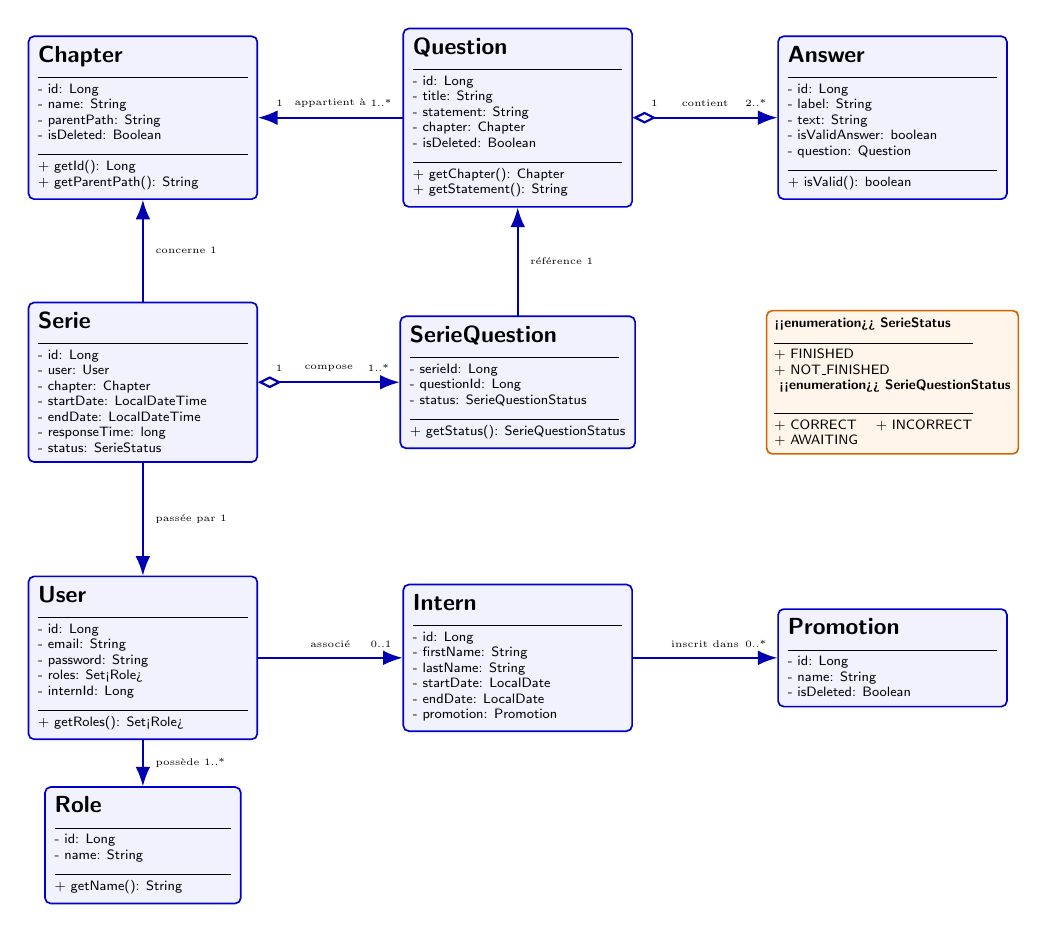
\begin{tikzpicture}[
    scale=0.70,
    transform shape,
    font=\sffamily\scriptsize,
    classbox/.style={draw=blue!80!black, fill=blue!5, rounded corners=2pt, align=left, inner sep=5pt, line width=0.6pt},
    enumbox/.style={draw=orange!80!black, fill=orange!8, rounded corners=2pt, align=left, inner sep=4pt, line width=0.6pt},
    assoc/.style={-{Latex[length=2.5mm]}, thick, draw=blue!70!black},
    comp/.style={{Diamond[open, length=3mm]}-{Latex[length=2.5mm]}, thick, draw=blue!70!black}
]

    % --- Ligne 1 : Connaissances & Questions ---
    \node[classbox, minimum width=4.0cm] (chapter) at (-6.8, 5.0) {
        \textbf{\large Chapter}\\
        \rule{3.8cm}{0.4pt}\\
        - id: Long\\
        - name: String\\
        - parentPath: String\\
        - isDeleted: Boolean\\
        \rule{3.8cm}{0.4pt}\\
        + getId(): Long\\
        + getParentPath(): String
    };

    \node[classbox, minimum width=4.0cm] (question) at (0.0, 5.0) {
        \textbf{\large Question}\\
        \rule{3.8cm}{0.4pt}\\
        - id: Long\\
        - title: String\\
        - statement: String\\
        - chapter: Chapter\\
        - isDeleted: Boolean\\
        \rule{3.8cm}{0.4pt}\\
        + getChapter(): Chapter\\
        + getStatement(): String
    };

    \node[classbox, minimum width=4.0cm] (answer) at (6.8, 5.0) {
        \textbf{\large Answer}\\
        \rule{3.8cm}{0.4pt}\\
        - id: Long\\
        - label: String\\
        - text: String\\
        - isValidAnswer: boolean\\
        - question: Question\\
        \rule{3.8cm}{0.4pt}\\
        + isValid(): boolean
    };

    % --- Ligne 2 : Séries d'examen & Entraînement ---
    \node[classbox, minimum width=4.0cm] (serie) at (-6.8, 0.2) {
        \textbf{\large Serie}\\
        \rule{3.8cm}{0.4pt}\\
        - id: Long\\
        - user: User\\
        - chapter: Chapter\\
        - startDate: LocalDateTime\\
        - endDate: LocalDateTime\\
        - responseTime: long\\
        - status: SerieStatus
    };

    \node[classbox, minimum width=4.0cm] (serieq) at (0.0, 0.2) {
        \textbf{\large SerieQuestion}\\
        \rule{3.8cm}{0.4pt}\\
        - serieId: Long\\
        - questionId: Long\\
        - status: SerieQuestionStatus\\
        \rule{3.8cm}{0.4pt}\\
        + getStatus(): SerieQuestionStatus
    };

    \node[enumbox, minimum width=3.8cm] (enum_seriestat) at (6.8, 0.2) {
        \textbf{<<enumeration>> SerieStatus}\\
        \rule{3.6cm}{0.4pt}\\
        + FINISHED\\
        + NOT\_FINISHED\\
        \vspace{3pt}
        \textbf{<<enumeration>> SerieQuestionStatus}\\
        \rule{3.6cm}{0.4pt}\\
        + CORRECT \quad + INCORRECT\\
        + AWAITING
    };

    % --- Ligne 3 : Utilisateurs & Promotion ---
    \node[classbox, minimum width=4.0cm] (user) at (-6.8, -4.8) {
        \textbf{\large User}\\
        \rule{3.8cm}{0.4pt}\\
        - id: Long\\
        - email: String\\
        - password: String\\
        - roles: Set<Role>\\
        - internId: Long\\
        \rule{3.8cm}{0.4pt}\\
        + getRoles(): Set<Role>
    };

    \node[classbox, minimum width=4.0cm] (intern) at (0.0, -4.8) {
        \textbf{\large Intern}\\
        \rule{3.8cm}{0.4pt}\\
        - id: Long\\
        - firstName: String\\
        - lastName: String\\
        - startDate: LocalDate\\
        - endDate: LocalDate\\
        - promotion: Promotion
    };

    \node[classbox, minimum width=4.0cm] (promo) at (6.8, -4.8) {
        \textbf{\large Promotion}\\
        \rule{3.8cm}{0.4pt}\\
        - id: Long\\
        - name: String\\
        - isDeleted: Boolean
    };

    \node[classbox, minimum width=3.4cm] (role) at (-6.8, -8.2) {
        \textbf{\large Role}\\
        \rule{3.2cm}{0.4pt}\\
        - id: Long\\
        - name: String\\
        \rule{3.2cm}{0.4pt}\\
        + getName(): String
    };

    % --- Relations avec étiquettes parfaitement positionnées et sans superposition ---
    \draw[assoc] (question.west) -- (chapter.east);
    \path (chapter.east) -- node[pos=0.15, above=2pt, font=\tiny] {1}
                           node[pos=0.5, above=2pt, font=\tiny] {appartient à}
                           node[pos=0.85, above=2pt, font=\tiny] {1..*} (question.west);

    \draw[comp] (question.east) -- (answer.west);
    \path (question.east) -- node[pos=0.15, above=2pt, font=\tiny] {1}
                            node[pos=0.5, above=2pt, font=\tiny] {contient}
                            node[pos=0.85, above=2pt, font=\tiny] {2..*} (answer.west);

    \draw[assoc] (serie.north) -- (chapter.south);
    \path (serie.north) -- node[midway, right=3pt, font=\tiny] {concerne 1} (chapter.south);

    \draw[comp] (serie.east) -- (serieq.west);
    \path (serie.east) -- node[pos=0.15, above=2pt, font=\tiny] {1}
                         node[pos=0.5, above=2pt, font=\tiny] {compose}
                         node[pos=0.85, above=2pt, font=\tiny] {1..*} (serieq.west);

    \draw[assoc] (serieq.north) -- (question.south);
    \path (serieq.north) -- node[midway, right=3pt, font=\tiny] {référence 1} (question.south);

    \draw[assoc] (serie.south) -- (user.north);
    \path (serie.south) -- node[midway, right=3pt, font=\tiny] {passée par 1} (user.north);

    \draw[assoc] (user.east) -- (intern.west);
    \path (user.east) -- node[pos=0.5, above=2pt, font=\tiny] {associé}
                        node[pos=0.85, above=2pt, font=\tiny] {0..1} (intern.west);

    \draw[assoc] (intern.east) -- (promo.west);
    \path (intern.east) -- node[pos=0.5, above=2pt, font=\tiny] {inscrit dans}
                          node[pos=0.85, above=2pt, font=\tiny] {0..*} (promo.west);

    \draw[assoc] (user.south) -- (role.north);
    \path (user.south) -- node[midway, right=3pt, font=\tiny] {possède 1..*} (role.north);

\end{tikzpicture}
\caption{Diagramme de classes UML du domaine métier de la plateforme d'évaluation (Backend)}
\label{fig:annexe_uml_domaine_quiz}
\end{figure}

\cleardoublepage

\section{Plateforme d'Évaluation : Architecture Logicielle en Couches et Aspects (Spring)}
\label{annexe:sec_uml_couches_quiz}

La Figure~\ref{fig:annexe_uml_couches_quiz} détaille le découpage en couches de l'application backend Java, illustrant le flux d'exécution type d'une requête REST (du contrôleur jusqu'à la base de données via DAOs et Repositories), ainsi que l'interception non-intrusive assurée par Spring AOP pour la journalisation, la sécurité et la métrologie de performance.

\begin{figure}[htbp]
\centering
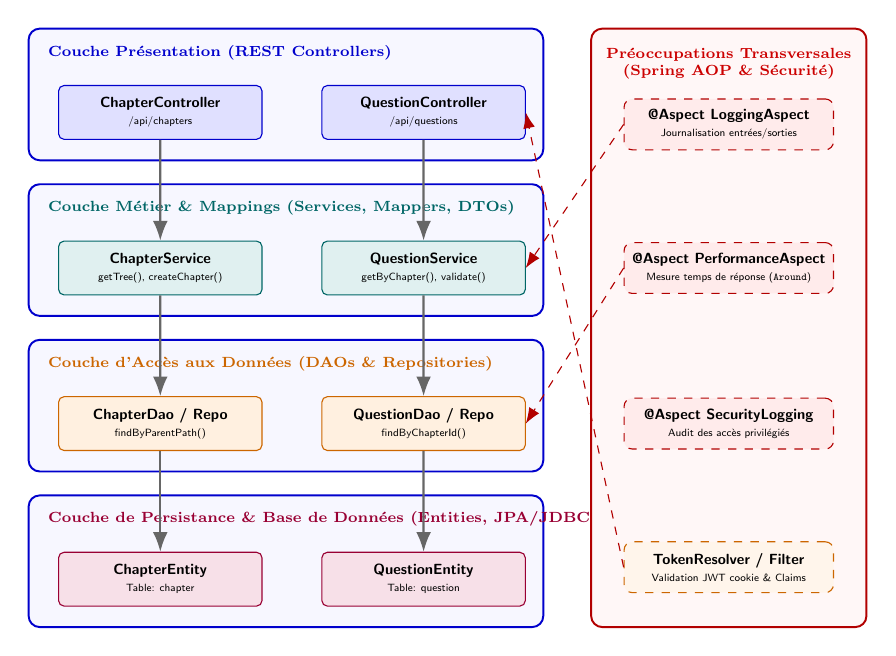
\begin{tikzpicture}[
    scale=0.76,
    transform shape,
    font=\sffamily\scriptsize,
    layer/.style={draw=blue!80!black, fill=blue!3, rounded corners=4pt, line width=0.7pt},
    compctrl/.style={draw=blue!80!black, fill=blue!12, rounded corners=2pt, minimum width=3.4cm, minimum height=0.9cm, align=center},
    compserv/.style={draw=teal!80!black, fill=teal!12, rounded corners=2pt, minimum width=3.4cm, minimum height=0.9cm, align=center},
    compdao/.style={draw=orange!80!black, fill=orange!12, rounded corners=2pt, minimum width=3.4cm, minimum height=0.9cm, align=center},
    compent/.style={draw=purple!80!black, fill=purple!12, rounded corners=2pt, minimum width=3.4cm, minimum height=0.9cm, align=center},
    aspectbox/.style={draw=red!70!black, fill=red!8, dashed, rounded corners=3pt, minimum width=3.5cm, minimum height=0.85cm, align=center},
    call/.style={-{Latex[length=2.5mm]}, thick, draw=gray!80!black}
]

    % Cadres des couches avec titre bien au-dessus
    \draw[layer] (-6.4, 6.0) rectangle (2.2, 3.8);
    \node[anchor=north west, font=\scriptsize\bfseries\color{blue!80!black}] at (-6.2, 5.85) {Couche Présentation (REST Controllers)};

    \draw[layer] (-6.4, 3.4) rectangle (2.2, 1.2);
    \node[anchor=north west, font=\scriptsize\bfseries\color{teal!80!black}] at (-6.2, 3.25) {Couche Métier \& Mappings (Services, Mappers, DTOs)};

    \draw[layer] (-6.4, 0.8) rectangle (2.2, -1.4);
    \node[anchor=north west, font=\scriptsize\bfseries\color{orange!80!black}] at (-6.2, 0.65) {Couche d'Accès aux Données (DAOs \& Repositories)};

    \draw[layer] (-6.4, -1.8) rectangle (2.2, -4.0);
    \node[anchor=north west, font=\scriptsize\bfseries\color{purple!80!black}] at (-6.2, -1.95) {Couche de Persistance \& Base de Données (Entities, JPA/JDBC)};

    % Composants Couche Présentation
    \node[compctrl] (ctrl_chap) at (-4.2, 4.6) {\textbf{ChapterController}\\ \tiny /api/chapters};
    \node[compctrl] (ctrl_quest) at (0.2, 4.6) {\textbf{QuestionController}\\ \tiny /api/questions};

    % Composants Couche Service
    \node[compserv] (serv_chap) at (-4.2, 2.0) {\textbf{ChapterService}\\ \tiny getTree(), createChapter()};
    \node[compserv] (serv_quest) at (0.2, 2.0) {\textbf{QuestionService}\\ \tiny getByChapter(), validate()};

    % Composants Couche DAO
    \node[compdao] (dao_chap) at (-4.2, -0.6) {\textbf{ChapterDao / Repo}\\ \tiny findByParentPath()};
    \node[compdao] (dao_quest) at (0.2, -0.6) {\textbf{QuestionDao / Repo}\\ \tiny findByChapterId()};

    % Composants Couche Entity
    \node[compent] (ent_chap) at (-4.2, -3.2) {\textbf{ChapterEntity}\\ \tiny Table: chapter};
    \node[compent] (ent_quest) at (0.2, -3.2) {\textbf{QuestionEntity}\\ \tiny Table: question};

    % Flux d'appels verticaux
    \draw[call] (ctrl_chap) -- (serv_chap);
    \draw[call] (ctrl_quest) -- (serv_quest);
    \draw[call] (serv_chap) -- (dao_chap);
    \draw[call] (serv_quest) -- (dao_quest);
    \draw[call] (dao_chap) -- (ent_chap);
    \draw[call] (dao_quest) -- (ent_quest);

    % Boîte Aspects Transverses (Spring AOP)
    \draw[draw=red!70!black, fill=red!3, rounded corners=4pt, line width=0.7pt] (3.0, 6.0) rectangle (7.6, -4.0);
    \node[anchor=north, font=\scriptsize\bfseries\color{red!80!black}, align=center] at (5.3, 5.8) {Préoccupations Transversales\\ (Spring AOP \& Sécurité)};

    \node[aspectbox] (asp_log) at (5.3, 4.4) {\textbf{@Aspect LoggingAspect}\\ \tiny Journalisation entrées/sorties};
    \node[aspectbox] (asp_perf) at (5.3, 2.0) {\textbf{@Aspect PerformanceAspect}\\ \tiny Mesure temps de réponse (\texttt{Around})};
    \node[aspectbox] (asp_sec) at (5.3, -0.6) {\textbf{@Aspect SecurityLogging}\\ \tiny Audit des accès privilégiés};
    \node[aspectbox, fill=orange!8, draw=orange!80!black] (jwt) at (5.3, -3.0) {\textbf{TokenResolver / Filter}\\ \tiny Validation JWT cookie \& Claims};

    % Liens de tissage AOP ciblés
    \draw[draw=red!70!black, dashed, -{Latex[length=2mm]}] (asp_log.west) -- (serv_quest.east);
    \draw[draw=red!70!black, dashed, -{Latex[length=2mm]}] (asp_perf.west) -- (dao_quest.east);
    \draw[draw=red!70!black, dashed, -{Latex[length=2mm]}] (jwt.west) -- (ctrl_quest.east);

\end{tikzpicture}
\caption{Architecture logicielle en couches et tissage des aspects transverses (Spring Core / AOP)}
\label{fig:annexe_uml_couches_quiz}
\end{figure}

\cleardoublepage

\section{Plateforme d'Évaluation : Architecture Frontend Réactive (Angular)}
\label{annexe:sec_uml_front_angular}

La Figure~\ref{fig:annexe_uml_front_angular} présente la structure de l'application cliente Angular du projet \code{newro-factory-front-avril}. Elle met en évidence l'architecture modulaire séparant les composants conteneurs dynamiques (\textit{Smart Components}), les composants de présentation réutilisables (\textit{Dumb Components}), ainsi que les services d'infrastructure et d'accès aux API distantes.

\begin{figure}[htbp]
\centering
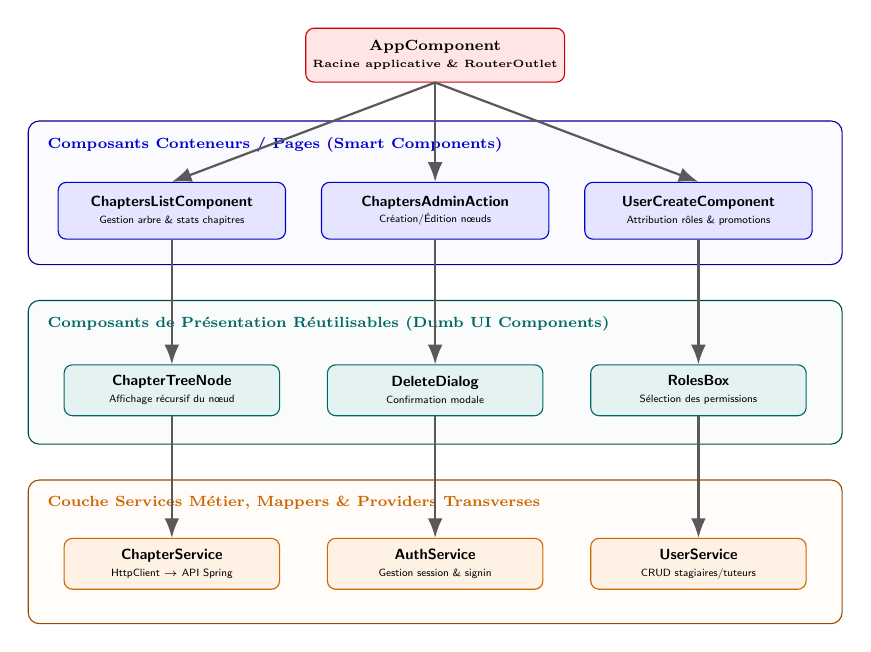
\begin{tikzpicture}[
    scale=0.76,
    transform shape,
    font=\sffamily\scriptsize,
    rootbox/.style={draw=red!80!black, fill=red!10, rounded corners=3pt, minimum width=3.8cm, minimum height=0.9cm, align=center, font=\scriptsize\bfseries},
    smartbox/.style={draw=blue!80!black, fill=blue!10, rounded corners=3pt, minimum width=3.8cm, minimum height=0.95cm, align=center},
    dumbbox/.style={draw=teal!80!black, fill=teal!10, rounded corners=3pt, minimum width=3.6cm, minimum height=0.85cm, align=center},
    servbox/.style={draw=orange!80!black, fill=orange!10, rounded corners=3pt, minimum width=3.6cm, minimum height=0.85cm, align=center},
    provbox/.style={draw=purple!80!black, fill=purple!10, rounded corners=3pt, minimum width=3.6cm, minimum height=0.85cm, align=center},
    wire/.style={-{Latex[length=2.5mm]}, thick, draw=gray!70!black}
]

    % Composant racine
    \node[rootbox] (app) at (0, 6.6) {AppComponent\\ \tiny Racine applicative \& RouterOutlet};

    % Smart Components
    \draw[draw=blue!60!black, fill=blue!2, rounded corners=4pt] (-6.8, 5.5) rectangle (6.8, 3.1);
    \node[anchor=north west, font=\scriptsize\bfseries\color{blue!80!black}] at (-6.6, 5.35) {Composants Conteneurs / Pages (Smart Components)};

    \node[smartbox] (c_chap) at (-4.4, 4.0) {\textbf{ChaptersListComponent}\\ \tiny Gestion arbre \& stats chapitres};
    \node[smartbox] (c_admin) at (0, 4.0) {\textbf{ChaptersAdminAction}\\ \tiny Création/Édition nœuds};
    \node[smartbox] (c_user) at (4.4, 4.0) {\textbf{UserCreateComponent}\\ \tiny Attribution rôles \& promotions};

    % Dumb Components
    \draw[draw=teal!60!black, fill=teal!2, rounded corners=4pt] (-6.8, 2.5) rectangle (6.8, 0.1);
    \node[anchor=north west, font=\scriptsize\bfseries\color{teal!80!black}] at (-6.6, 2.35) {Composants de Présentation Réutilisables (Dumb UI Components)};

    \node[dumbbox] (d_tree) at (-4.4, 1.0) {\textbf{ChapterTreeNode}\\ \tiny Affichage récursif du nœud};
    \node[dumbbox] (d_dialog) at (0, 1.0) {\textbf{DeleteDialog}\\ \tiny Confirmation modale};
    \node[dumbbox] (d_roles) at (4.4, 1.0) {\textbf{RolesBox}\\ \tiny Sélection des permissions};

    % Services HTTP & Providers
    \draw[draw=orange!60!black, fill=orange!2, rounded corners=4pt] (-6.8, -0.5) rectangle (6.8, -2.9);
    \node[anchor=north west, font=\scriptsize\bfseries\color{orange!80!black}] at (-6.6, -0.65) {Couche Services Métier, Mappers \& Providers Transverses};

    \node[servbox] (s_chap) at (-4.4, -1.9) {\textbf{ChapterService}\\ \tiny HttpClient $\rightarrow$ API Spring};
    \node[servbox] (s_auth) at (0, -1.9) {\textbf{AuthService}\\ \tiny Gestion session \& signin};
    \node[servbox] (s_user) at (4.4, -1.9) {\textbf{UserService}\\ \tiny CRUD stagiaires/tuteurs};

    % Liens verticaux directs par colonne (aucun croisement)
    \draw[wire] (app.south) -- (c_chap.north);
    \draw[wire] (app.south) -- (c_admin.north);
    \draw[wire] (app.south) -- (c_user.north);

    \draw[wire] (c_chap.south) -- (d_tree.north);
    \draw[wire] (c_admin.south) -- (d_dialog.north);
    \draw[wire] (c_user.south) -- (d_roles.north);

    \draw[wire] (d_tree.south) -- (s_chap.north);
    \draw[wire] (d_dialog.south) -- (s_auth.north);
    \draw[wire] (d_roles.south) -- (s_user.north);

\end{tikzpicture}
\caption{Architecture des composants réactifs et des flux de services (Angular Standalone)}
\label{fig:annexe_uml_front_angular}
\end{figure}

\cleardoublepage

\section{Usine Logicielle : Patrons de Conception et Abstractions des Fournisseurs}
\label{annexe:sec_uml_usine_patterns}

La Figure~\ref{fig:annexe_uml_usine_patterns} expose les diagrammes de classes UML régissant le découplage technologique de l'usine logicielle du projet \code{usine-logicielle}. On y retrouve l'application combinée des patrons \textit{Adapter}, \textit{Factory/Resolver} et \textit{Branded Types} pour garantir l'interchangeabilité des forges logicielles (\code{BacklogProvider}, \code{CodeBaseProvider}) sans couplage fort avec les librairies externes.

\begin{figure}[htbp]
\centering
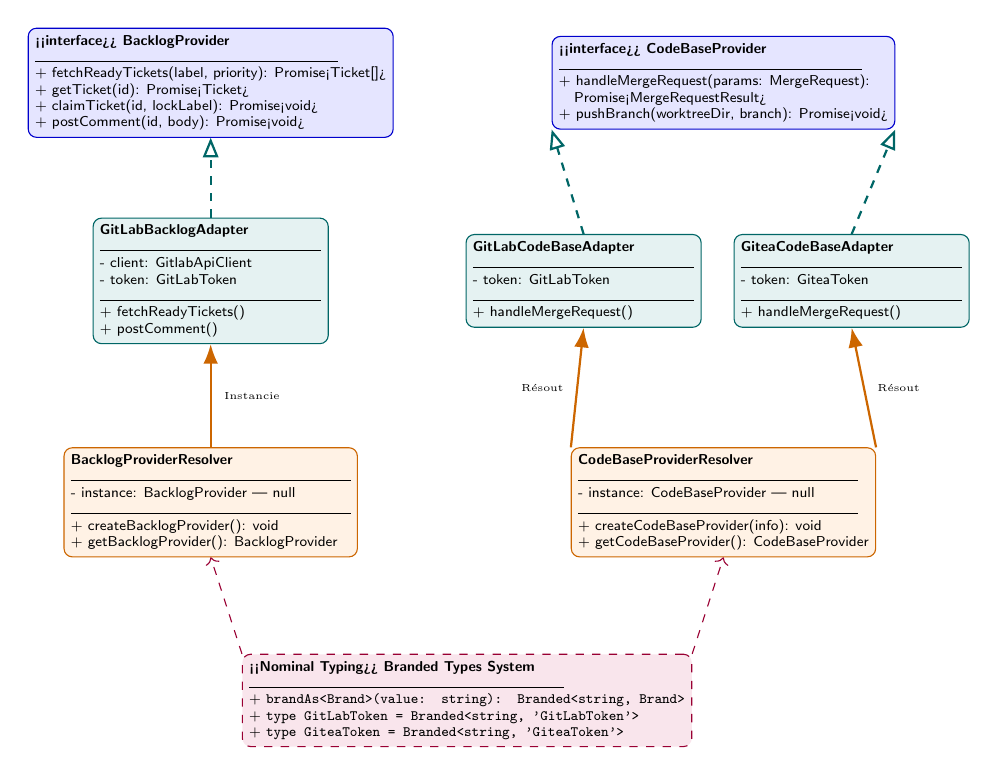
\begin{tikzpicture}[
    scale=0.74,
    transform shape,
    font=\sffamily\scriptsize,
    intbox/.style={draw=blue!80!black, fill=blue!10, rounded corners=3pt, minimum width=5.4cm, minimum height=1.4cm, align=left},
    adapbox/.style={draw=teal!80!black, fill=teal!10, rounded corners=3pt, minimum width=4.0cm, minimum height=1.3cm, align=left},
    factbox/.style={draw=orange!80!black, fill=orange!10, rounded corners=3pt, minimum width=5.0cm, minimum height=1.2cm, align=left},
    brandbox/.style={draw=purple!80!black, fill=purple!10, dashed, rounded corners=3pt, minimum width=5.6cm, minimum height=1.4cm, align=left},
    arrow/.style={-{Latex[length=2.5mm]}, thick, draw=orange!80!black},
    impl/.style={-{Triangle[open, length=2.5mm]}, dashed, thick, draw=teal!80!black}
]

    % Interfaces de Fournisseurs (Ligne 1)
    \node[intbox] (backlog_int) at (-4.4, 5.6) {
        \textbf{<<interface>> BacklogProvider}\\
        \rule{5.2cm}{0.4pt}\\
        + fetchReadyTickets(label, priority): Promise<Ticket[]>\\
        + getTicket(id): Promise<Ticket>\\
        + claimTicket(id, lockLabel): Promise<void>\\
        + postComment(id, body): Promise<void>
    };

    \node[intbox] (codebase_int) at (4.4, 5.6) {
        \textbf{<<interface>> CodeBaseProvider}\\
        \rule{5.2cm}{0.4pt}\\
        + handleMergeRequest(params: MergeRequest):\\
        \quad Promise<MergeRequestResult>\\
        + pushBranch(worktreeDir, branch): Promise<void>
    };

    % Adaptateurs Concrets (Ligne 2)
    \node[adapbox] (gitlab_back) at (-4.4, 2.2) {
        \textbf{GitLabBacklogAdapter}\\
        \rule{3.8cm}{0.4pt}\\
        - client: GitlabApiClient\\
        - token: GitLabToken\\
        \rule{3.8cm}{0.4pt}\\
        + fetchReadyTickets()\\
        + postComment()
    };

    \node[adapbox] (gitlab_code) at (2.0, 2.2) {
        \textbf{GitLabCodeBaseAdapter}\\
        \rule{3.8cm}{0.4pt}\\
        - token: GitLabToken\\
        \rule{3.8cm}{0.4pt}\\
        + handleMergeRequest()
    };

    \node[adapbox] (gitea_code) at (6.6, 2.2) {
        \textbf{GiteaCodeBaseAdapter}\\
        \rule{3.8cm}{0.4pt}\\
        - token: GiteaToken\\
        \rule{3.8cm}{0.4pt}\\
        + handleMergeRequest()
    };

    % Resolvers / Factory (Ligne 3 avec espacement vertical)
    \node[factbox] (backlog_res) at (-4.4, -1.6) {
        \textbf{BacklogProviderResolver}\\
        \rule{4.8cm}{0.4pt}\\
        - instance: BacklogProvider | null\\
        \rule{4.8cm}{0.4pt}\\
        + createBacklogProvider(): void\\
        + getBacklogProvider(): BacklogProvider
    };

    \node[factbox] (codebase_res) at (4.4, -1.6) {
        \textbf{CodeBaseProviderResolver}\\
        \rule{4.8cm}{0.4pt}\\
        - instance: CodeBaseProvider | null\\
        \rule{4.8cm}{0.4pt}\\
        + createCodeBaseProvider(info): void\\
        + getCodeBaseProvider(): CodeBaseProvider
    };

    % Branded Types Box (Ligne 4 bien séparée)
    \node[brandbox] (brands) at (0.0, -5.0) {
        \textbf{<<Nominal Typing>> Branded Types System}\\
        \rule{5.4cm}{0.4pt}\\
        + \texttt{brandAs<Brand>(value: string): Branded<string, Brand>}\\
        + \texttt{type GitLabToken = Branded<string, 'GitLabToken'>}\\
        + \texttt{type GiteaToken = Branded<string, 'GiteaToken'>}
    };

    % Liens d'implémentation
    \draw[impl] (gitlab_back.north) -- (backlog_int.south);
    \draw[impl] (gitlab_code.north) -- (codebase_int.south west);
    \draw[impl] (gitea_code.north) -- (codebase_int.south east);

    % Liens des Factory
    \draw[arrow] (backlog_res.north) -- node[right=3pt, font=\tiny] {Instancie} (gitlab_back.south);
    \draw[arrow] (codebase_res.north west) -- node[left=3pt, font=\tiny] {Résout} (gitlab_code.south);
    \draw[arrow] (codebase_res.north east) -- node[right=3pt, font=\tiny] {Résout} (gitea_code.south);

    % Liens Branded Types
    \draw[draw=purple!80!black, dashed, ->] (brands.north west) -- (backlog_res.south);
    \draw[draw=purple!80!black, dashed, ->] (brands.north east) -- (codebase_res.south);

\end{tikzpicture}
\caption{Diagramme de classes UML des abstractions et adaptateurs de forges (Usine Logicielle)}
\label{fig:annexe_uml_usine_patterns}
\end{figure}

\cleardoublepage

\section{Usine Logicielle : Moteurs de Validation Mécanique et Cycle du Worker}
\label{annexe:sec_uml_usine_worker}

La Figure~\ref{fig:annexe_uml_usine_worker} schématise l'organisation interne du moteur d'exécution (\texttt{Worker}) et de ses garde-fous mécaniques, garantissant l'étanchéité contextuelle et la résilience aux pannes via la persistance d'états dans le fichier \code{manifest.json}.

\begin{figure}[htbp]
\centering
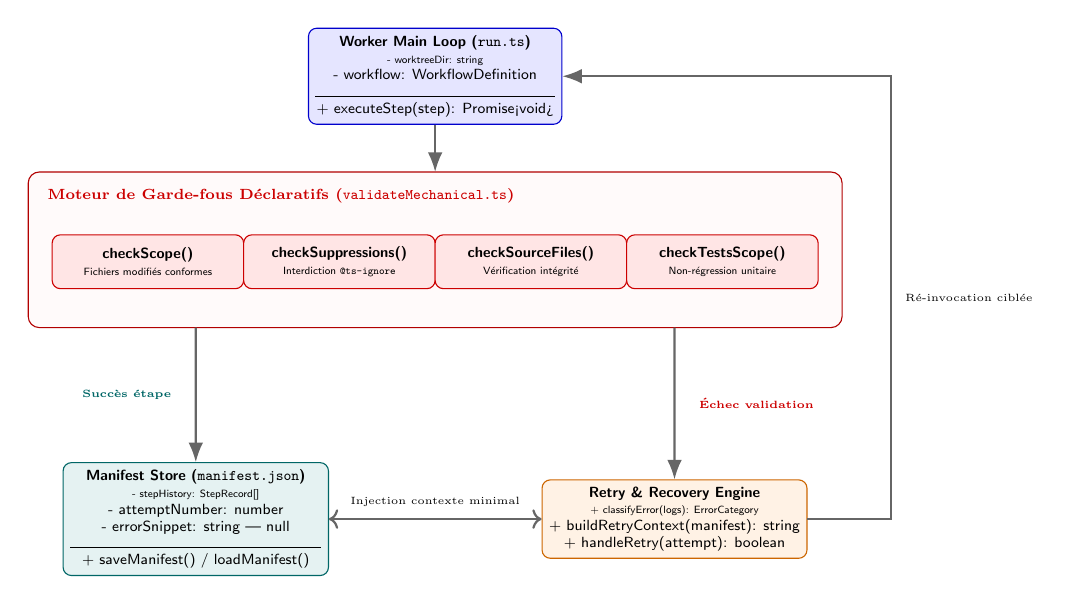
\begin{tikzpicture}[
    scale=0.76,
    transform shape,
    font=\sffamily\scriptsize,
    corebox/.style={draw=blue!80!black, fill=blue!10, rounded corners=3pt, minimum width=4.2cm, minimum height=1.1cm, align=center},
    guardbox/.style={draw=red!80!black, fill=red!10, rounded corners=3pt, minimum width=3.2cm, minimum height=0.9cm, align=center},
    manifestbox/.style={draw=teal!80!black, fill=teal!10, rounded corners=3pt, minimum width=4.4cm, minimum height=1.1cm, align=center},
    retrybox/.style={draw=orange!80!black, fill=orange!10, rounded corners=3pt, minimum width=4.2cm, minimum height=1.1cm, align=center},
    arrow/.style={-{Latex[length=2.5mm]}, thick, draw=gray!80!black}
]

    % Composant central Worker
    \node[corebox] (worker) at (0, 6.2) {
        \textbf{Worker Main Loop (\texttt{run.ts})}\\
        \tiny - worktreeDir: string\\
        - workflow: WorkflowDefinition\\
        \rule{4.0cm}{0.4pt}\\
        + executeStep(step): Promise<void>
    };

    % Moteur de Garde-fous mécaniques
    \draw[draw=red!70!black, fill=red!2, rounded corners=4pt] (-6.8, 4.6) rectangle (6.8, 2.0);
    \node[anchor=north west, font=\scriptsize\bfseries\color{red!80!black}] at (-6.6, 4.45) {Moteur de Garde-fous Déclaratifs (\texttt{validateMechanical.ts})};

    \node[guardbox] (g_scope) at (-4.8, 3.1) {\textbf{checkScope()}\\ \tiny Fichiers modifiés conformes};
    \node[guardbox] (g_supp) at (-1.6, 3.1) {\textbf{checkSuppressions()}\\ \tiny Interdiction \texttt{@ts-ignore}};
    \node[guardbox] (g_src) at (1.6, 3.1) {\textbf{checkSourceFiles()}\\ \tiny Vérification intégrité};
    \node[guardbox] (g_tests) at (4.8, 3.1) {\textbf{checkTestsScope()}\\ \tiny Non-régression unitaire};

    % Persistance d'état & Manifest (parfaitement alignés sous les garde-fous)
    \node[manifestbox] (manifest) at (-4.0, -1.2) {
        \textbf{Manifest Store (\texttt{manifest.json})}\\
        \tiny - stepHistory: StepRecord[]\\
        - attemptNumber: number\\
        - errorSnippet: string | null\\
        \rule{4.2cm}{0.4pt}\\
        + saveManifest() / loadManifest()
    };

    % Moteur de Réessai et Classification
    \node[retrybox] (retry) at (4.0, -1.2) {
        \textbf{Retry \& Recovery Engine}\\
        \tiny + classifyError(logs): ErrorCategory\\
        + buildRetryContext(manifest): string\\
        + handleRetry(attempt): boolean
    };

    % Relations et flux (droits et verticaux, zéro collision)
    \draw[arrow] (worker.south) -- (0, 4.6);

    \draw[arrow] (-4.0, 2.0) -- node[midway, left=8pt, font=\tiny\bfseries\color{teal!80!black}] {Succès étape} (manifest.north);
    \draw[arrow] (4.0, 2.0) -- node[midway, right=8pt, font=\tiny\bfseries\color{red!80!black}] {Échec validation} (retry.north);

    \draw[arrow, <->] (manifest.east) -- node[above=2pt, font=\tiny] {Injection contexte minimal} (retry.west);
    \draw[arrow] (retry.east) -- ++(1.4,0) |- node[pos=0.25, right=3pt, font=\tiny] {Ré-invocation ciblée} (worker.east);

\end{tikzpicture}
\caption{Architecture du moteur de validation mécanique et boucle de réessai du Worker}
\label{fig:annexe_uml_usine_worker}
\end{figure}
\cleardoublepage

\chapter{Exemples de traces d'exécution de l'usine logicielle}
\label{annexe:traces}

Cette annexe présente un relevé exhaustif de journaux d'audit (\textit{execution logs}) générés en environnement conteneurisé lors du traitement automatisé d'un ticket d'ingénierie (Ticket~\#17 : \og \textit{Fix element picker: escape key does not deactivate element picker} \fg{}).

Les événements sont émis au format JSON Lines structuré, intégrant l'horodatage ISO-8601 (\code{ts}), le niveau de sévérité (\code{level}), le composant émetteur (\code{component} : \code{supervisor} ou \code{worker}), l'identifiant d'exécution unique (\code{runId}), ainsi que les métriques et métadonnées d'étape.

\section{Journal brut d'exécution (Format JSON Lines)}
\label{annexe:sec_logs_bruts}

Le Listing~\ref{lst:logs_usine_ticket17} reproduit la séquence complète des logs, depuis la finalisation du plan d'action jusqu'à la détection de défaillance d'authentification lors de l'étape finale d'intégration Git.

\begin{lstlisting}[basicstyle=\ttfamily\fontsize{6.5pt}{7.5pt}\selectfont, breaklines=true, frame=single, caption={Extrait des traces d'exécution de l'usine logicielle sur le Ticket \#17}, label={lst:logs_usine_ticket17}]
usine-usine  | {"ts":"2026-08-27T15:58:00.937Z","level":"INFO","component":"worker","msg":"Claude execution completed","runId":"1017-17-20260827T155453Z","stepId":"plan","exitCode":0,"outputLength":409,"output":"Ticket #17's implementation plan is ready in .task/plan.md. It covers: adding an ELEMENT_PICKER_CANCEL endpoint, a new cancel handler in both the content-script and background element picker controllers, an Escape-key listener in Chat.vue (sidebar) gated on picker-active state with proper mount/unmount cleanup, and matching test cases in Chat.spec.ts. No source files were modified -- just the plan.\n","stderrLength":0,"stderrlog":""}
usine-usine  | {"ts":"2026-08-27T15:58:00.938Z","level":"DEBUG","component":"worker","msg":"Global attempt incremented","runId":"1017-17-20260827T155453Z","total":2}
usine-usine  | {"ts":"2026-08-27T15:58:00.939Z","level":"DEBUG","component":"worker","msg":"Mechanical validation passed","runId":"1017-17-20260827T155453Z","stepId":"plan"}
usine-usine  | {"ts":"2026-08-27T15:58:00.939Z","level":"INFO","component":"worker","msg":"Step execution completed","runId":"1017-17-20260827T155453Z","stepId":"plan","success":true,"exitCode":0}
usine-usine  | {"ts":"2026-08-27T15:58:01.159Z","level":"WARN","component":"worker","msg":"Commit failed","runId":"1017-17-20260827T155453Z","stepId":"plan","error":"Command failed: git commit -m usine: plan -- success"}
usine-usine  | {"ts":"2026-08-27T15:58:01.161Z","level":"INFO","component":"worker","msg":"Step notification","runId":"1017-17-20260827T155453Z","stepId":"plan","status":"success","durationMs":65220,"nextStepId":"code-full"}
usine-usine  | {"ts":"2026-08-27T15:58:01.161Z","level":"DEBUG","component":"worker","msg":"Execution log appended","runId":"1017-17-20260827T155453Z","stepId":"plan","totalEntries":2}
usine-usine  | {"ts":"2026-08-27T15:58:01.170Z","level":"DEBUG","component":"worker","msg":"Manifest saved","runId":"1017-17-20260827T155453Z","path":"/repo/.worktrees/17/.task/manifest.json","currentStep":"code-full"}
usine-usine  | {"ts":"2026-08-27T15:58:01.170Z","level":"INFO","component":"worker","msg":"=== Step starting","runId":"1017-17-20260827T155453Z","stepId":"code-full","index":2,"dispatchReason":"initial"}
usine-usine  | {"ts":"2026-08-27T15:58:01.174Z","level":"DEBUG","component":"worker","msg":"Step execution starting","runId":"1017-17-20260827T155453Z","stepId":"code-full","type":"prompt"}
usine-usine  | {"ts":"2026-08-27T15:58:01.174Z","level":"DEBUG","component":"worker","msg":"Tools allocated for step","runId":"1017-17-20260827T155453Z","stepId":"code-full","tools":["Read","Write","Glob","Grep","Bash","Edit","Task"]}
usine-usine  | {"ts":"2026-08-27T15:58:01.175Z","level":"INFO","component":"worker","msg":"Executing prompt step","runId":"1017-17-20260827T155453Z","stepId":"code-full","command":"/code-full","tools":7}
usine-usine  | {"ts":"2026-08-27T15:58:01.177Z","level":"DEBUG","component":"worker","msg":"Spawning claude CLI (prompt sent via stdin)","runId":"1017-17-20260827T155453Z","binary":"claude","args":["--print","--output-format","text","--verbose","--session-id","777a71ca-b8ce-4507-9876-669a2d2aee47","--allowed-tools","Read,Write,Glob,Grep,Bash,Edit,Task"]}
usine-usine  | {"ts":"2026-08-27T15:58:06.263Z","level":"DEBUG","component":"supervisor","msg":"Poll cycle #20","activeWorkers":1,"inFlightTickets":1}
usine-usine  | {"ts":"2026-08-27T15:58:26.267Z","level":"DEBUG","component":"supervisor","msg":"Poll cycle #21","activeWorkers":1,"inFlightTickets":1}
usine-usine  | {"ts":"2026-08-27T15:58:46.275Z","level":"DEBUG","component":"supervisor","msg":"Poll cycle #22","activeWorkers":1,"inFlightTickets":1}
usine-usine  | {"ts":"2026-08-27T15:59:06.272Z","level":"DEBUG","component":"supervisor","msg":"Poll cycle #23","activeWorkers":1,"inFlightTickets":1}
usine-usine  | {"ts":"2026-08-27T15:59:26.278Z","level":"DEBUG","component":"supervisor","msg":"Poll cycle #24","activeWorkers":1,"inFlightTickets":1}
usine-usine  | {"ts":"2026-08-27T15:59:27.354Z","level":"DEBUG","component":"supervisor","msg":"found workflow: usine-PIerreV::full for ticket id=17","id":17}
usine-usine  | {"ts":"2026-08-27T15:59:27.359Z","level":"DEBUG","component":"supervisor","msg":"[ELIGIBILITY] #17 rejete par \"is_not_claimed\": label claimed:* present","iid":17,"rule":"is_not_claimed"}
usine-usine  | {"ts":"2026-08-27T15:59:46.288Z","level":"DEBUG","component":"supervisor","msg":"Poll cycle #25","activeWorkers":1,"inFlightTickets":1}
usine-usine  | {"ts":"2026-08-27T15:59:47.172Z","level":"DEBUG","component":"supervisor","msg":"found workflow: usine-PIerreV::full for ticket id=17","id":17}
usine-usine  | {"ts":"2026-08-27T15:59:47.173Z","level":"DEBUG","component":"supervisor","msg":"[ELIGIBILITY] #17 rejete par \"is_not_claimed\": label claimed:* present","iid":17,"rule":"is_not_claimed"}
usine-usine  | {"ts":"2026-08-27T16:00:06.296Z","level":"DEBUG","component":"supervisor","msg":"Poll cycle #26","activeWorkers":1,"inFlightTickets":1}
usine-usine  | {"ts":"2026-08-27T16:00:07.026Z","level":"DEBUG","component":"supervisor","msg":"found workflow: usine-PIerreV::full for ticket id=17","id":17}
usine-usine  | {"ts":"2026-08-27T16:00:07.026Z","level":"DEBUG","component":"supervisor","msg":"[ELIGIBILITY] #17 rejete par \"is_not_claimed\": label claimed:* present","iid":17,"rule":"is_not_claimed"}
usine-usine  | {"ts":"2026-08-27T16:00:26.307Z","level":"DEBUG","component":"supervisor","msg":"Poll cycle #27","activeWorkers":1,"inFlightTickets":1}
usine-usine  | {"ts":"2026-08-27T16:00:27.265Z","level":"DEBUG","component":"supervisor","msg":"found workflow: usine-PIerreV::full for ticket id=17","id":17}
usine-usine  | {"ts":"2026-08-27T16:00:27.265Z","level":"DEBUG","component":"supervisor","msg":"[ELIGIBILITY] #17 rejete par \"is_not_claimed\": label claimed:* present","iid":17,"rule":"is_not_claimed"}
usine-usine  | {"ts":"2026-08-27T16:00:46.315Z","level":"DEBUG","component":"supervisor","msg":"Poll cycle #28","activeWorkers":1,"inFlightTickets":1}
usine-usine  | {"ts":"2026-08-27T16:00:47.417Z","level":"DEBUG","component":"supervisor","msg":"found workflow: usine-PIerreV::full for ticket id=17","id":17}
usine-usine  | {"ts":"2026-08-27T16:00:47.418Z","level":"DEBUG","component":"supervisor","msg":"[ELIGIBILITY] #17 rejete par \"is_not_claimed\": label claimed:* present","iid":17,"rule":"is_not_claimed"}
usine-usine  | {"ts":"2026-08-27T16:01:06.315Z","level":"DEBUG","component":"supervisor","msg":"Poll cycle #29","activeWorkers":1,"inFlightTickets":1}
usine-usine  | {"ts":"2026-08-27T16:01:07.107Z","level":"DEBUG","component":"supervisor","msg":"found workflow: usine-PIerreV::full for ticket id=17","id":17}
usine-usine  | {"ts":"2026-08-27T16:01:07.108Z","level":"DEBUG","component":"supervisor","msg":"[ELIGIBILITY] #17 rejete par \"is_not_claimed\": label claimed:* present","iid":17,"rule":"is_not_claimed"}
usine-usine  | {"ts":"2026-08-27T16:01:26.185Z","level":"INFO","component":"supervisor","msg":"isAlive","activeWorkers":1,"inFlightTickets":1}
usine-usine  | {"ts":"2026-08-27T16:01:26.318Z","level":"DEBUG","component":"supervisor","msg":"Poll cycle #30","activeWorkers":1,"inFlightTickets":1}
usine-usine  | {"ts":"2026-08-27T16:01:27.407Z","level":"DEBUG","component":"supervisor","msg":"found workflow: usine-PIerreV::full for ticket id=17","id":17}
usine-usine  | {"ts":"2026-08-27T16:01:27.409Z","level":"DEBUG","component":"supervisor","msg":"[ELIGIBILITY] #17 rejete par \"is_not_claimed\": label claimed:* present","iid":17,"rule":"is_not_claimed"}
usine-usine  | {"ts":"2026-08-27T16:01:41.120Z","level":"INFO","component":"worker","msg":"Claude execution completed","runId":"1017-17-20260827T155453Z","stepId":"code-full","exitCode":0,"outputLength":1268,"output":"Ticket #17 implemented by the code-full subagent in two phases.\n\n**Source changes** (Escape key now deactivates the element picker):\n- Endpoint.enum.ts -- new ELEMENT_PICKER_CANCEL endpoint\n- content-script/.../ElementPicker.controller.ts -- cancelPicker handler calling the idempotent deactivatePickMode()\n- background/controllers/ElementPicker.controller.ts -- forwardCancelToTab forwarding to the active tab (mirrors forwardStartToTab)\n- sidebar/front/components/chat/Chat.vue -- isPickerActive ref, window keydown listener sending ELEMENT_PICKER_CANCEL on Escape only when active, cleaned up in new onBeforeUnmount\n\n**Tests**: new tests/components/chat/Chat.elementPicker.spec.ts -- 5 tests (START on activation, CANCEL on active Escape, no CANCEL when inactive, single-fire on repeated Escape, listener cleanup on unmount).\n\n**Limitation flagged by the subagent**: the worktree has no node_modules and npm install fails offline, so build/lint/type-check/tests were **not executed**. The spec mirrors the existing working Chat.spec.ts scaffold, but someone needs to run npm test in a provisioned environment to confirm green + coverage.\n\nReports written to .task/code-report.md, .task/test-report.md, .task/staged-files.txt.\n","stderrLength":0,"stderrlog":""}
usine-usine  | {"ts":"2026-08-27T16:01:41.120Z","level":"DEBUG","component":"worker","msg":"Global attempt incremented","runId":"1017-17-20260827T155453Z","total":3}
usine-usine  | {"ts":"2026-08-27T16:01:42.187Z","level":"DEBUG","component":"worker","msg":"Mechanical validation passed","runId":"1017-17-20260827T155453Z","stepId":"code-full"}
usine-usine  | {"ts":"2026-08-27T16:01:42.187Z","level":"INFO","component":"worker","msg":"Step execution completed","runId":"1017-17-20260827T155453Z","stepId":"code-full","success":true,"exitCode":0}
usine-usine  | {"ts":"2026-08-27T16:01:42.552Z","level":"INFO","component":"worker","msg":"Progress committed","runId":"1017-17-20260827T155453Z","stepId":"code-full","sha":"ae722be9"}
usine-usine  | {"ts":"2026-08-27T16:01:43.003Z","level":"WARN","component":"worker","msg":"Push failed (commit only)","runId":"1017-17-20260827T155453Z","stepId":"code-full"}
usine-usine  | {"ts":"2026-08-27T16:01:43.009Z","level":"INFO","component":"worker","msg":"Step notification","runId":"1017-17-20260827T155453Z","stepId":"code-full","status":"success","durationMs":219946,"nextStepId":"push"}
usine-usine  | {"ts":"2026-08-27T16:01:43.011Z","level":"DEBUG","component":"worker","msg":"Execution log appended","runId":"1017-17-20260827T155453Z","stepId":"code-full","totalEntries":3}
usine-usine  | {"ts":"2026-08-27T16:01:43.037Z","level":"DEBUG","component":"worker","msg":"Manifest saved","runId":"1017-17-20260827T155453Z","path":"/repo/.worktrees/17/.task/manifest.json","currentStep":"push"}
usine-usine  | {"ts":"2026-08-27T16:01:43.037Z","level":"INFO","component":"worker","msg":"=== Step starting","runId":"1017-17-20260827T155453Z","stepId":"push","index":3,"dispatchReason":"initial"}
usine-usine  | {"ts":"2026-08-27T16:01:43.041Z","level":"DEBUG","component":"worker","msg":"Step execution starting","runId":"1017-17-20260827T155453Z","stepId":"push","type":"script"}
usine-usine  | {"ts":"2026-08-27T16:01:43.057Z","level":"INFO","component":"worker","msg":"Executing script step","runId":"1017-17-20260827T155453Z","stepId":"push","commandCount":4,"preview":"git rm -r --cached .task/ 2>/dev/null || true; git add $(cat .task/staged-files.txt)"}
usine-usine  | {"ts":"2026-08-27T16:01:43.604Z","level":"WARN","component":"worker","msg":"Script execution failed","runId":"1017-17-20260827T155453Z","stepId":"push","exitCode":128,"output":"","error":"+ git rm -r --cached .task/\n+ true\n++ cat .task/staged-files.txt\n+ git add src/common/shared/models/Endpoint.enum.ts src/content-script/content/controllers/ElementPicker.controller.ts src/background/controllers/ElementPicker.controller.ts src/sidebar/front/components/chat/Chat.vue tests/components/chat/Chat.elementPicker.spec.ts\n+ git diff --cached --quiet\n+ git push --force origin 17-fix-element-picker-escape-key-does-not-deactivate-element-pi\nfatal: could not read Username for 'https://git.oxyl.fr': No such device or address\n","failedCommand":"git push --force origin 17-fix-element-picker-escape-key-does-not-deactivate-element-pi"}
usine-usine  | {"ts":"2026-08-27T16:01:43.606Z","level":"DEBUG","component":"worker","msg":"Global attempt incremented","runId":"1017-17-20260827T155453Z","total":4}
usine-usine  | {"ts":"2026-08-27T16:01:43.607Z","level":"INFO","component":"worker","msg":"Step execution completed","runId":"1017-17-20260827T155453Z","stepId":"push","success":false,"exitCode":128}
usine-usine  | {"ts":"2026-08-27T16:01:43.610Z","level":"INFO","component":"worker","msg":"Failure classified","runId":"1017-17-20260827T155453Z","stepId":"push","category":"unknown","isRetryable":false}
usine-usine  | {"ts":"2026-08-27T16:01:43.611Z","level":"INFO","component":"worker","msg":"Retrying step","runId":"1017-17-20260827T155453Z","stepId":"push","retryCount":1,"maxRetries":2}
usine-usine  | {"ts":"2026-08-27T16:01:43.612Z","level":"DEBUG","component":"worker","msg":"Retry count incremented","runId":"1017-17-20260827T155453Z","stepId":"push","count":1}
usine-usine  | {"ts":"2026-08-27T16:01:43.630Z","level":"DEBUG","component":"worker","msg":"Manifest saved","runId":"1017-17-20260827T155453Z","path":"/repo/.worktrees/17/.task/manifest.json","currentStep":"push"}
usine-usine  | {"ts":"2026-08-27T16:01:43.632Z","level":"INFO","component":"worker","msg":"Retrying step (1/2)","runId":"1017-17-20260827T155453Z","stepId":"push"}
usine-usine  | {"ts":"2026-08-27T16:01:43.636Z","level":"INFO","component":"worker","msg":"=== Step starting","runId":"1017-17-20260827T155453Z","dispatchReason":"retry (1/2)","stepId":"push","index":3}
usine-usine  | {"ts":"2026-08-27T16:01:43.636Z","level":"DEBUG","component":"worker","msg":"Step execution starting","runId":"1017-17-20260827T155453Z","dispatchReason":"retry (1/2)","stepId":"push","type":"script"}
usine-usine  | {"ts":"2026-08-27T16:01:43.659Z","level":"INFO","component":"worker","msg":"Executing script step","runId":"1017-17-20260827T155453Z","dispatchReason":"retry (1/2)","stepId":"push","commandCount":4,"preview":"git rm -r --cached .task/ 2>/dev/null || true; git add $(cat .task/staged-files.txt)"}
usine-usine  | {"ts":"2026-08-27T16:01:44.052Z","level":"WARN","component":"worker","msg":"Script execution failed","runId":"1017-17-20260827T155453Z","dispatchReason":"retry (1/2)","stepId":"push","exitCode":128,"output":"","error":"+ git rm -r --cached .task/\n+ true\n++ cat .task/staged-files.txt\n+ git add src/common/shared/models/Endpoint.enum.ts src/content-script/content/controllers/ElementPicker.controller.ts src/background/controllers/ElementPicker.controller.ts src/sidebar/front/components/chat/Chat.vue tests/components/chat/Chat.elementPicker.spec.ts\n+ git diff --cached --quiet\n+ git push --force origin 17-fix-element-picker-escape-key-does-not-deactivate-element-pi\nfatal: could not read Username for 'https://git.oxyl.fr': No such device or address\n","failedCommand":"git push --force origin 17-fix-element-picker-escape-key-does-not-deactivate-element-pi"}
usine-usine  | {"ts":"2026-08-27T16:01:44.052Z","level":"DEBUG","component":"worker","msg":"Global attempt incremented","runId":"1017-17-20260827T155453Z","dispatchReason":"retry (1/2)","total":5}
usine-usine  | {"ts":"2026-08-27T16:01:44.052Z","level":"INFO","component":"worker","msg":"Step execution completed","runId":"1017-17-20260827T155453Z","dispatchReason":"retry (1/2)","stepId":"push","success":false,"exitCode":128}
usine-usine  | {"ts":"2026-08-27T16:01:44.053Z","level":"INFO","component":"worker","msg":"Failure classified","runId":"1017-17-20260827T155453Z","dispatchReason":"retry (1/2)","stepId":"push","category":"unknown","isRetryable":false}
usine-usine  | {"ts":"2026-08-27T16:01:44.055Z","level":"INFO","component":"worker","msg":"Retrying step","runId":"1017-17-20260827T155453Z","dispatchReason":"retry (1/2)","stepId":"push","retryCount":2,"maxRetries":2}
usine-usine  | {"ts":"2026-08-27T16:01:44.055Z","level":"DEBUG","component":"worker","msg":"Retry count incremented","runId":"1017-17-20260827T155453Z","dispatchReason":"retry (1/2)","stepId":"push","count":2}
usine-usine  | {"ts":"2026-08-27T16:01:44.069Z","level":"DEBUG","component":"worker","msg":"Manifest saved","runId":"1017-17-20260827T155453Z","dispatchReason":"retry (1/2)","path":"/repo/.worktrees/17/.task/manifest.json","currentStep":"push"}
usine-usine  | {"ts":"2026-08-27T16:01:44.071Z","level":"INFO","component":"worker","msg":"Retrying step (2/2)","runId":"1017-17-20260827T155453Z","dispatchReason":"retry (1/2)","stepId":"push"}
usine-usine  | {"ts":"2026-08-27T16:01:44.072Z","level":"INFO","component":"worker","msg":"=== Step starting","runId":"1017-17-20260827T155453Z","dispatchReason":"retry (2/2)","stepId":"push","index":3}
usine-usine  | {"ts":"2026-08-27T16:01:44.072Z","level":"DEBUG","component":"worker","msg":"Step execution starting","runId":"1017-17-20260827T155453Z","dispatchReason":"retry (2/2)","stepId":"push","type":"script"}
usine-usine  | {"ts":"2026-08-27T16:01:44.072Z","level":"INFO","component":"worker","msg":"Executing script step","runId":"1017-17-20260827T155453Z","dispatchReason":"retry (2/2)","stepId":"push","commandCount":4,"preview":"git rm -r --cached .task/ 2>/dev/null || true; git add $(cat .task/staged-files.txt)"}
usine-usine  | {"ts":"2026-08-27T16:01:44.322Z","level":"WARN","component":"worker","msg":"Script execution failed","runId":"1017-17-20260827T155453Z","dispatchReason":"retry (2/2)","stepId":"push","exitCode":128,"output":"","error":"+ git rm -r --cached .task/\n+ true\n++ cat .task/staged-files.txt\n+ git add src/common/shared/models/Endpoint.enum.ts src/content-script/content/controllers/ElementPicker.controller.ts src/background/controllers/ElementPicker.controller.ts src/sidebar/front/components/chat/Chat.vue tests/components/chat/Chat.elementPicker.spec.ts\n+ git diff --cached --quiet\n+ git push --force origin 17-fix-element-picker-escape-key-does-not-deactivate-element-pi\nfatal: could not read Username for 'https://git.oxyl.fr': No such device or address\n","failedCommand":"git push --force origin 17-fix-element-picker-escape-key-does-not-deactivate-element-pi"}
usine-usine  | {"ts":"2026-08-27T16:01:44.322Z","level":"DEBUG","component":"worker","msg":"Global attempt incremented","runId":"1017-17-20260827T155453Z","dispatchReason":"retry (2/2)","total":6}
usine-usine  | {"ts":"2026-08-27T16:01:44.323Z","level":"INFO","component":"worker","msg":"Step execution completed","runId":"1017-17-20260827T155453Z","dispatchReason":"retry (2/2)","stepId":"push","success":false,"exitCode":128}
usine-usine  | {"ts":"2026-08-27T16:01:44.323Z","level":"INFO","component":"worker","msg":"Failure classified","runId":"1017-17-20260827T155453Z","dispatchReason":"retry (2/2)","stepId":"push","category":"unknown","isRetryable":false}
usine-usine  | {"ts":"2026-08-27T16:01:44.325Z","level":"WARN","component":"worker","msg":"max_on_fail reached for script step, exiting","runId":"1017-17-20260827T155453Z","dispatchReason":"retry (2/2)","stepId":"push","onFailCount":0,"maxOnFail":null}
usine-usine  | {"ts":"2026-08-27T16:01:44.326Z","level":"INFO","component":"worker","msg":"[X] Step failed: Max retries reached for step push (2)","runId":"1017-17-20260827T155453Z","dispatchReason":"retry (2/2)","stepId":"push","exitCode":1,"durationMs":250}
\end{lstlisting}

\section{Analyse détaillée des jalons de l'exécution}
\label{annexe:sec_analyse_jalons}

L'examen pas-à-pas de ce journal d'audit confirme l'application effective des principes architecturaux détaillés dans les Chapitres~\ref{chap:usine_ia} et~\ref{chap:infra_agnostique} :

\begin{enumerate}
    \item \textbf{Gestion distribuée de la concurrence (Superviseur) :}
    Les lignes émises par le composant \code{supervisor} démontrent l'efficacité de la règle d'exclusion mutuelle \code{is_not_claimed}. Alors que le worker exécute les sous-étapes dans son \textit{Git Worktree} isolé, le superviseur détecte le ticket \#17 à chaque cycle de scrutation (\code{Poll cycle \#20} à \code{\#30}) mais ignore son traitement car le label de verrouillage (\code{claimed:*}) est actif.

    \item \textbf{Étanchéité et formalisation de la phase de planification (\texttt{plan}) :}
    L'étape \code{plan} instancie Claude CLI avec des arguments explicites (\code{--session-id}, \code{--allowed-tools}). L'agent formalise le plan dans \code{.task/plan.md} sans toucher au code source. Le moteur applique ensuite la validation mécanique (\code{Mechanical validation passed}), enregistre l'état dans \code{manifest.json} et ordonnance le passage à l'étape suivante.

    \item \textbf{Cloisonnement de l'outillage et traçabilité documentaire (\texttt{code-full}) :}
    L'étape d'implémentation ouvre l'outil d'édition (\code{Edit}) parmi les 7 outils autorisés. L'agent réalise les modifications sur 4 fichiers sources et rédige un fichier de test dédié (\code{Chat.elementPicker.spec.ts}). L'agent note explicitement l'environnement hermétique (\textit{offline}) du conteneur empêchant l'installation de dépendances npm, consignant cette remarque dans \code{.task/code-report.md}. Un commit de progrès est scellé sous le SHA \code{ae722be9}.

    \item \textbf{Gouvernance déterministe et disjoncteur face aux erreurs (\texttt{push}) :}
    Lors de l'étape finale scriptée, la commande \code{git push} échoue par absence d'identifiants interactifs (erreur Git standard en environnement d'intégration non configuré). Le moteur de résilience classifie l'erreur, incrémente les compteurs de réessai (\code{retryCount: 1} puis \code{2}) et interrompt proprement la chaîne lorsque le seuil est atteint (\code{Max retries reached}), évitant tout blocage indéfini du conteneur.
\end{enumerate}

\cleardoublepage

\chapter{Vues d'écrans et Interfaces complémentaires de la plateforme NewroFactory}
\label{annexe:interfaces_quiz}

Cette annexe rassemble les captures d'écran des interfaces d'authentification, d'administration et de catalogue de la plateforme web \textit{NewroFactory}, complétant les vues fonctionnelles présentées au Chapitre~\ref{chap:quiz}.

\section{Authentification et Contrôle d'accès}
\label{annexe:sec_login}

La Figure~\ref{fig:ui_annexe_login} présente la page d'accueil et d'authentification de la plateforme, garantissant un accès sécurisé et cloisonné selon les rôles attribués (\code{ROLE_USER} ou \code{ROLE_ADMIN}).

\begin{figure}[htbp]
    \centering
    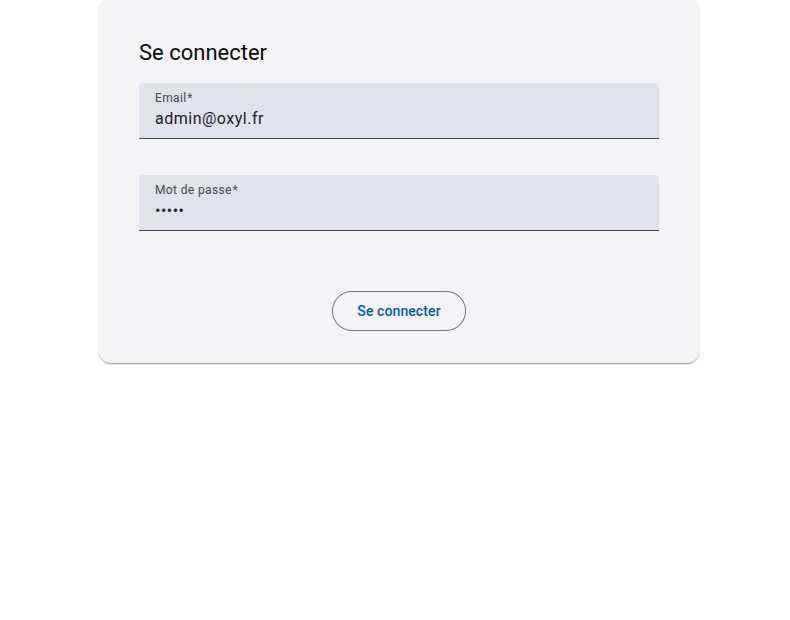
\includegraphics[width=0.68\textwidth]{figures/quiz_login.png}
    \caption{Page d'authentification et de connexion sécurisée à la plateforme NewroFactory}
    \label{fig:ui_annexe_login}
\end{figure}

\section{Tableau de bord général de supervision administrateur}
\label{annexe:sec_admin_dash}

La Figure~\ref{fig:ui_annexe_dashboard} illustre le tableau de bord d'accueil de l'administrateur et encadrant technique, consolidant les indicateurs clés (volume de compétences, nombre d'utilisateurs et de stagiaires actifs) et proposant des raccourcis vers les modules de gouvernance.

\begin{figure}[htbp]
    \centering
    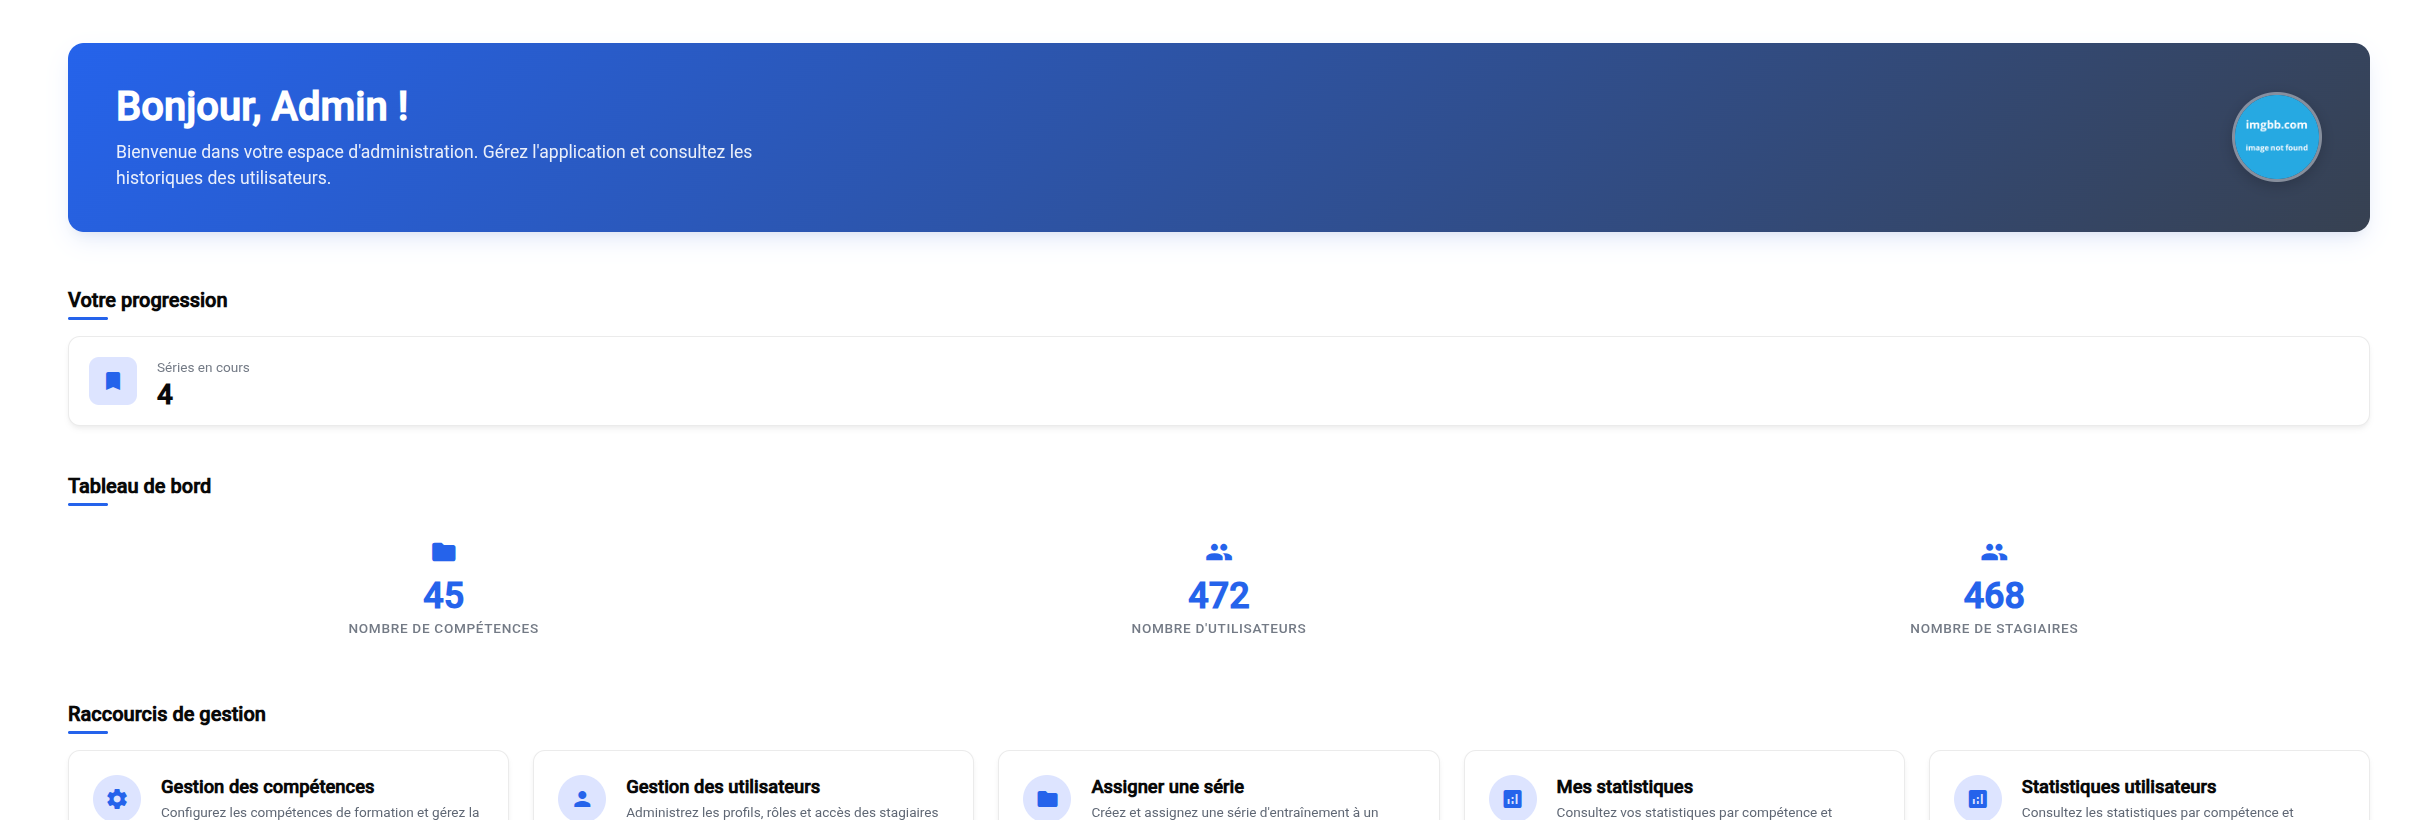
\includegraphics[width=0.92\textwidth]{figures/quiz_admin_dashboard.png}
    \caption{Tableau de bord général de l'administrateur avec métriques consolidées et raccourcis de gouvernance}
    \label{fig:ui_annexe_dashboard}
\end{figure}

\section{Référentiel des compétences et modules de formation}
\label{annexe:sec_competences_list}

La Figure~\ref{fig:ui_annexe_competences} présente le catalogue centralisé des compétences et certifications gérées sur la plateforme (Vue.js, Java OCA, Java OCP, Asynchronisme, ES6-ES11, Node CLI, Event Loop, File System, Process/OS, Spring Framework).

\begin{figure}[htbp]
    \centering
    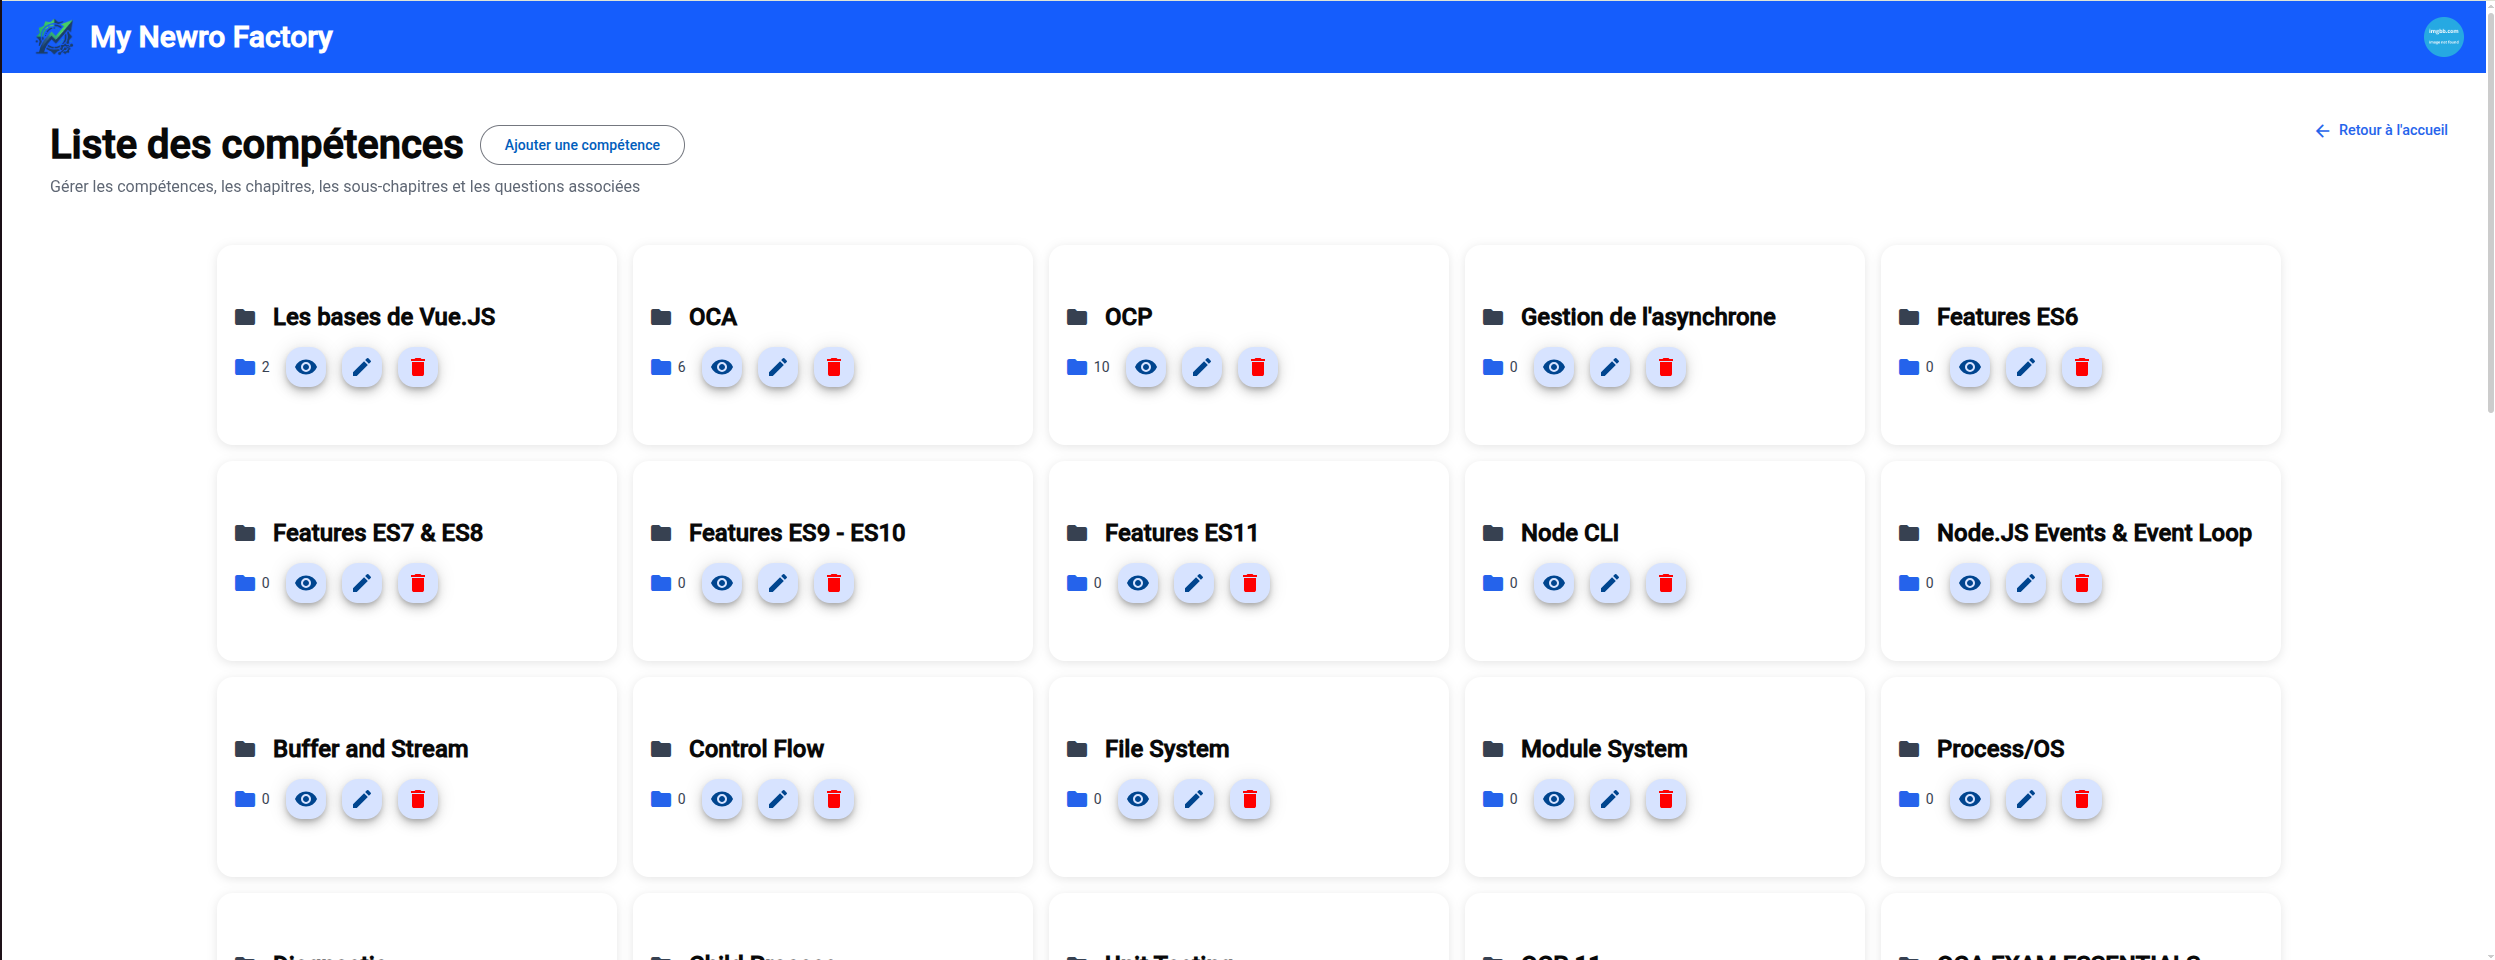
\includegraphics[width=0.92\textwidth]{figures/quiz_competences_list.png}
    \caption{Catalogue et référentiel des compétences de formation et modules d'évaluation}
    \label{fig:ui_annexe_competences}
\end{figure}

\section{Historique global et filtrage multicritères des séries}
\label{annexe:sec_stats_toutes_series}

La Figure~\ref{fig:ui_annexe_toutes_series} présente l'interface d'historique exhaustif des séries d'entraînement, dotée d'un curseur de filtrage interactif par taux de réussite (0\% à 100\%) et de mécanismes de tri chronologique.

\begin{figure}[htbp]
    \centering
    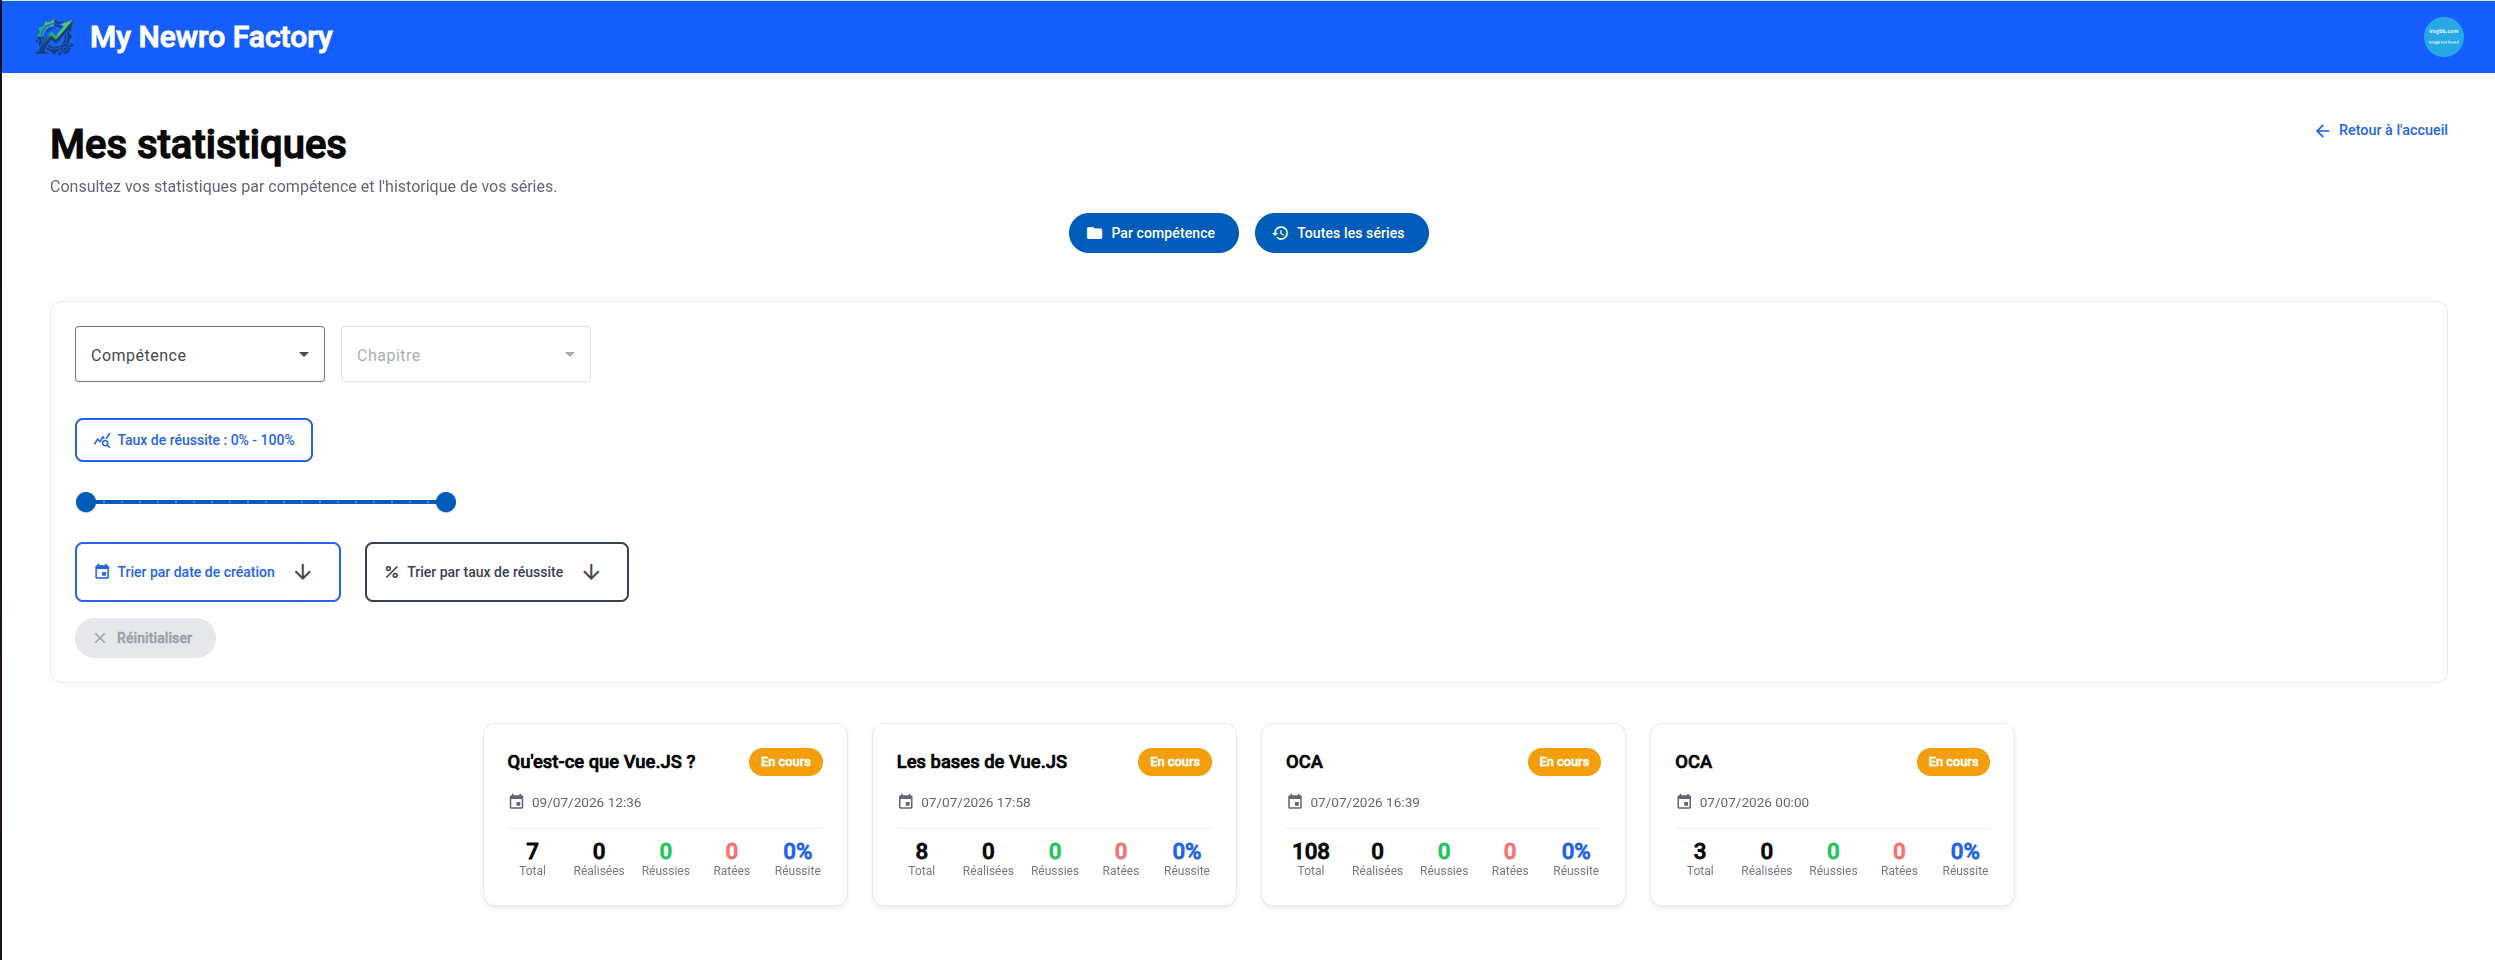
\includegraphics[width=0.92\textwidth]{figures/quiz_stats_toutes_series.png}
    \caption{Interface de consultation et de filtrage dynamique de l'historique complet des séries}
    \label{fig:ui_annexe_toutes_series}
\end{figure}

\cleardoublepage
\thispagestyle{empty}

\section*{Résumé}
\addcontentsline{toc}{chapter}{Résumé}

Dans un secteur des Entreprises de Services du Numérique (ESN) en pleine mutation vers les engagements au forfait et confronté à l'avènement de l'intelligence artificielle générative, la rentabilité et l'excellence technique imposent une refonte des chaînes de production logicielle. Ce mémoire présente les travaux d'ingénierie menés au sein du Groupe Oxyl, articulés autour d'une double industrialisation : celle du \textbf{capital humain} et celle du \textbf{capital technique}.

Le premier volet formalise la standardisation des compétences à travers la conception d'une plateforme d'évaluation et de préparation aux certifications industrielles (Oracle OCP Java, AWS), architecturée en Spring Core et Angular. Le second volet porte sur le développement d'une \textbf{usine logicielle agentique} en TypeScript, orchestrant des agents d'IA autonomes pour la résolution automatisée de tickets de développement et de maintenance. Afin de prévenir tout verrouillage propriétaire (\textit{vendor lock-in}), une couche d'abstraction logicielle fondée sur les patrons de conception (\textit{Factory}, \textit{Adapter}, \textit{Strategy}) garantit une stricte indépendance vis-à-vis des modèles de langage (LLM) et des forges logicielles (GitLab, GitHub, Jira).

L'analyse démontre la synergie fondamentale entre ces deux piliers : loin de remplacer l'ingénieur, l'usine logicielle déplace sa charge cognitive vers l'architecture et l'arbitrage critique, exigeant une maîtrise théorique accrue pour superviser le code généré. Cette approche hybride optimise les coûts d'inférence, réduit le coût de non-qualité et pérennise l'avance technologique et l'attractivité commerciale de l'entreprise.

\vspace{0.3cm}
{\bf Mots-clés :} Génie Logiciel, Usine Logicielle, Agents IA, Modèles de Langage (LLM), Agnosticisme Technologique, Patrons de Conception, Capital Humain, Certifications Java (OCP), Spring Core, Angular, TypeScript.


\section*{Abstract}
\addcontentsline{toc}{chapter}{Abstract}

In the IT services and consulting industry (ESN), driven by an accelerated shift towards fixed-price engagements and the rise of generative artificial intelligence, sustained profitability and technical excellence require a comprehensive industrialization of software engineering workflows. This master's thesis presents the engineering achievements developed within Groupe Oxyl, structured around a dual-pillar strategy: the industrialization of \textbf{human capital} and \textbf{technical capital}.

The first pillar formalizes skills standardization through the design of a training and certification assessment platform (Oracle OCP Java, AWS), engineered with Spring Core and Angular. The second pillar focuses on the development of an \textbf{agentic software factory} in TypeScript, orchestrating autonomous AI agents to resolve development and maintenance tickets. To prevent vendor lock-in, an abstraction layer based on design patterns (\textit{Factory}, \textit{Adapter}, \textit{Strategy}) ensures complete architectural independence from large language model (LLM) providers and software forges (GitLab, GitHub, Jira).

The analysis highlights the systemic synergy between both pillars: rather than replacing the engineer, the software factory elevates the cognitive workload toward architecture, specification, and critical review, demanding deeper theoretical mastery to supervise machine-generated code. This hybrid approach optimizes inference costs, mitigates the cost of non-quality, and secures a lasting technological edge and commercial attractiveness for the enterprise.

\vspace{0.3cm}
{\bf Keywords :} Software Engineering, Software Factory, AI Agents, Large Language Models (LLM), Vendor Lock-in Prevention, Design Patterns, Human Capital, Java Certification (OCP), Spring Core, Angular, TypeScript.

\end{document}
